\documentclass[11pt]{article}
\usepackage[scaled=0.92]{helvet}
\usepackage{geometry}
\geometry{letterpaper,tmargin=1in,bmargin=1in,lmargin=1in,rmargin=1in}
\usepackage[parfill]{parskip} % Activate to begin paragraphs with an empty line rather than an indent %\usepackage{graphicx}
\usepackage{amsmath,amssymb, mathrsfs, dsfont}
\usepackage{tabularx}
\usepackage[font=footnotesize,labelfont=bf]{caption}
\usepackage{graphicx}
\usepackage{xcolor}
%\usepackage[linkbordercolor ={1 1 1} ]{hyperref}
%\usepackage[sf]{titlesec}
\usepackage{natbib}
\usepackage{../../Tianpei_Report}
%\usepackage{appendix}
%\usepackage{algorithm}
%\usepackage{algorithmic}

%\renewcommand{\algorithmicrequire}{\textbf{Input:}}
%\renewcommand{\algorithmicensure}{\textbf{Output:}}



\begin{document}
\title{Self-study: fundamental of differential geometry for curves and surfaces}
\author{ Tianpei Xie}
\date{ Jun. 1st., 2015 }
\maketitle
\tableofcontents
\newpage
\section{Definitions and concepts}
\subsection{Curves}
\begin{itemize}
\item \begin{definition}
A \emph{parameterized differentiable curve} \citep{do1976differential} is a differentiable map $\alpha: I \rightarrow \bR^{3}$ of an open interval $I = (a,b) \subset \bR$ to $\bR^{3}$. 

 A parameterized curve is said to be \emph{regular} if $\alpha'(t)\neq 0$ for all $t\in I$.
\end{definition}

\item The \emph{arc length} of a regular parameterized curve $\alpha: I \rightarrow \bR^{3}$ from $t_{0}$ is defined as
\begin{align*}
s &\equiv \int_{t_{0}}^{t}\abs{\alpha'(t)} dt 
\end{align*} where $\abs{\alpha'(t)} = \sqrt{(x'(t))^{2} + (y'(t))^{2}+ (z'(t))^{2}}$. Note that a parameterized regular curve can be reparameterized by the arc length as $\alpha(s)$.

\item   \begin{definition}
The quantity $\abs{\alpha''(s)} \equiv k(s)$ is referred as the \emph{curvature} of $\alpha(s)$ at $s$. The curvature measures \emph{the rate of change} of the tangent line along the curve. 

 The differential of $\alpha(s)$ as $\mb{t}(s) \equiv \overrightarrow{t}(s) \equiv \alpha'(s)$ is the \emph{tangent vector} (velocity) of $\alpha(s)$ at $s$. 
\end{definition}

\item The acceleration vector $\alpha''(s)$ is orthogonal to the tangent vector and it is computed as $\alpha''(s) = k(s)\,\mb{n}(s)$, where $k(s)$ is the curvature and $\mb{n}(s) \equiv \overrightarrow{n}(s)$ is the \emph{normal vector} and it perpendicular to the tangent vector. 

\item \begin{definition}
The vector $\mb{b}(s) = \mb{t}(s) \wedge \mb{n}(s)$ is referred as the \emph{binormal vector}. It is the normal vector of the $t-n$ plane and it is orthogonal to $(\mb{t}, \mb{n})$. 
\end{definition}

\item The differential of binormal vector $\mb{b}'(s)$ characterize the strength of the curve to pull away from the plane where it currently lies. $\mb{b}'(s)$ is parallel to $\mb{n}(s)$ and is computed as $\mb{b}'(s) = \tau(s)\,\mb{n}(s)$ \citep{do1976differential}. (Some book use $\mb{b}'(s) = -\tau(s)\,\mb{n}(s)$. )

\item If $k(s)\neq 0$ for all $s\in I$, we could define the quantity $\tau(s)$ as the \emph{torsion} of $\alpha(s)$ at $s$. If $\tau \equiv 0$, then the curve will lies entirely in a plane and vise versa.   Note that $k(s)\neq 0$ is essential for above argument to hold. The sign of torsion is related to the orientation of the curve relative to the osculating plane. 

\item Both $k(s)$ and $\tau(s)$ are invariant to change of orientation. 

\item  \begin{definition}
The three orthonormal vectors $(\mb{t}(s), \mb{n}(s), \mb{b}(s))$ form a basis that uniquely characterizes the local behavior of a curve, and it is called the \emph{Frenet trihedron} at $s$. The curvature $k$ and the torsion $\tau$ will reveal information of curve $\alpha$ in the neighborhood of $s$.

\begin{figure}[tb]
\begin{minipage}{0.7\linewidth}
 \centerline{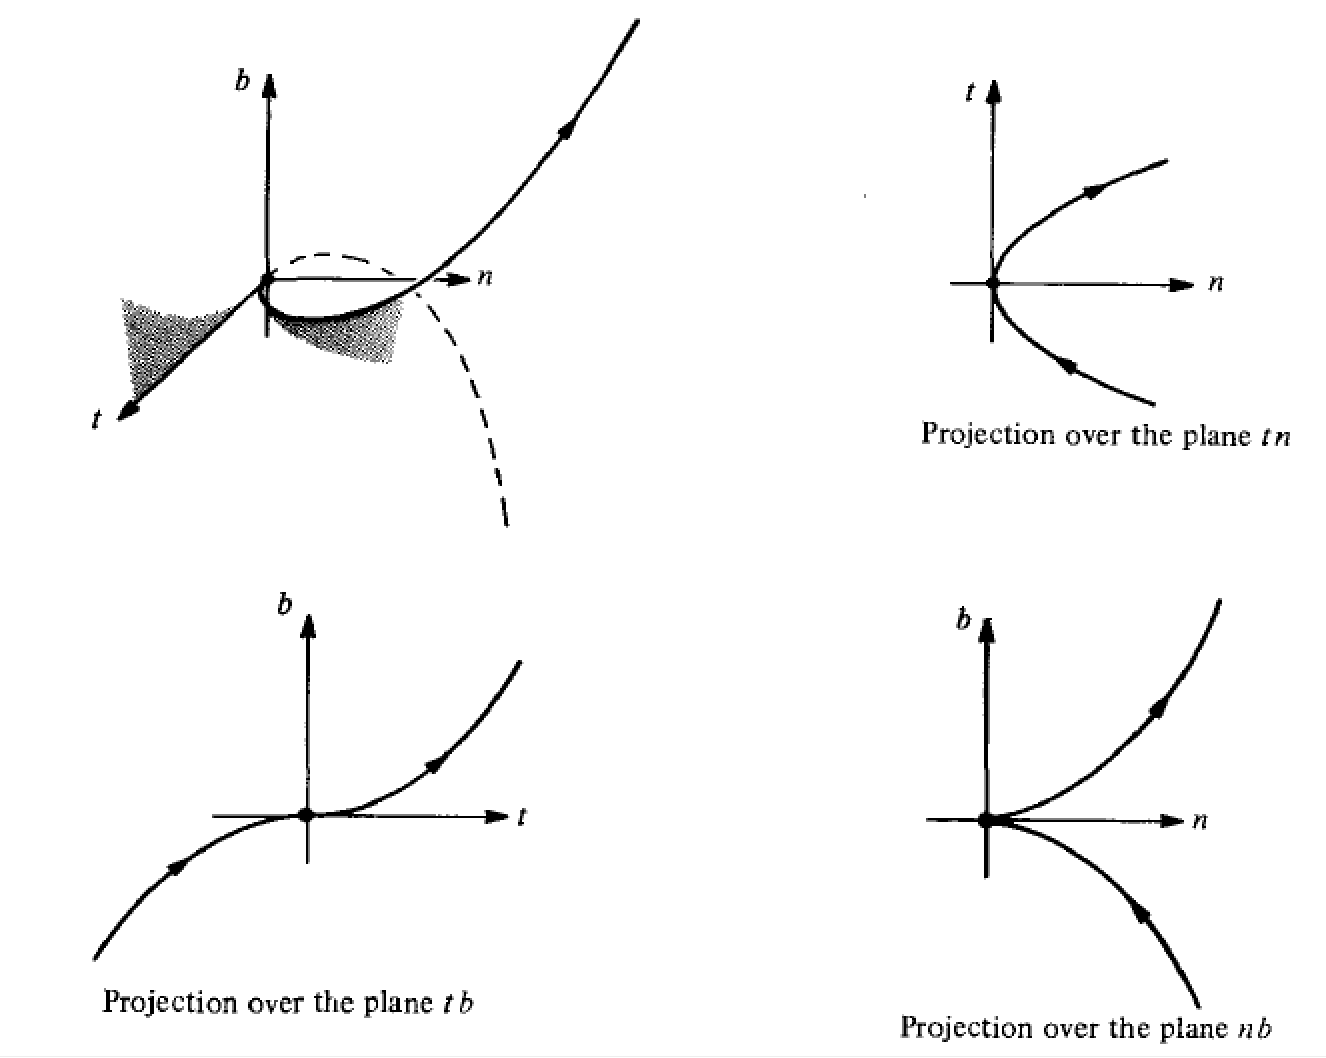
\includegraphics[scale = 0.5]{Frenet_trihedron.png}}
\end{minipage}
\caption{\scriptsize
\textbf{The local behavior of general regular curve. At the osculating plane, it is like a parabola. At the normal plane, it is like a cubic function. }}
\end{figure}
\end{definition}

\item Given $\tau(s)$ and $k(s)$, the curve at $s$ can be reparameterized via the trihedron $(\mb{t}, \mb{n}, \mb{b})$. 

\item \begin{definition}
The plane spanned by $(\mb{t, n})$ is called \emph{osculating plane}. The plane spanned by $(\mb{n, b})$ is called \emph{normal plane} and the plane spanned by $(\mb{t, b})$ is called \emph{rectifying plane}.
\end{definition}

%\item For any closed parameterized convex curve, the curvature $k(s)$ is nonnegative and has two maxima and two minima or is constant everywhere. \\[-5pt]
\end{itemize}\vspace{-15pt}
\subsection{Surfaces}
\begin{itemize}
\item \begin{definition}
A subset $\cS \subset \bR^{3}$ is a \emph{regular surface} \citep{do1976differential}, if for any $p\in \cS$, there exists a neighborhood $V \subset \bR^{3}$ and a map $\mb{x}: U \subset \mb{R}^{2} \rightarrow V\cap \cS$ of an open subset $U\subset \mb{R}^{2}$ onto $V \cap \cS \subset \bR^{3}$ such that 
\begin{enumerate}
\item $\mb{x}:  (u,v) \in U \rightarrow  (x(u,v), y(u,v), z(u,v))$ has differentials in $U$ with all orders. 
\item $\mb{x}$ is a homemorphism, i.e. $\mb{x}$ is a continuous bijection with continuous inverse $\mb{x}^{-1}: W \supset V\cap \cS \rightarrow \bR^{2}$.
\item For any $q\in U$, the differential $d\mb{x}_{q}$ is one-to-one, i.e. injective.   
\end{enumerate}   
Note: $dx_{q} \equiv \partdiff{(x,y,z)}{(u,v)} = \brac{\partdiff{x^{i}(\xi_{1},\xi_{2})}{\xi_{j}}}_{i,j} \in \bR^{3\times 2}$ with $x_{i} \in \set{x,y,z}$ and $\xi_{j}\in \set{u,v}$. And $dx_{q}$ is injective iff $\partdiff{(x,y,z)}{(u,v)}$ has full column rank. \\
\end{definition}

\item \begin{definition}
The map $\mb{x}: U\subset \bR^{2} \rightarrow V\cap \cS$ is called a \emph{parameterization} of the surface (at $p$). Its inverse $\mb{x}^{-1}: W\supset V\cap \cS \rightarrow U$ is called a \emph{coordinate system}. We may write $\mb{x}^{-1} = (u, v)$, where $u,v$ are smooth function on $W$ and are called \emph{coordinate functions} (\emph{local coordinate} of surface at $p$ as $p= (u,v)$). The neighborhood $V\cap \cS$ of $p$ is called the coordinate neighborhood of $p$ in $\cS$. 
\end{definition}
\begin{figure}[htb]
\centering
\begin{minipage}{0.6\linewidth}
 \centerline{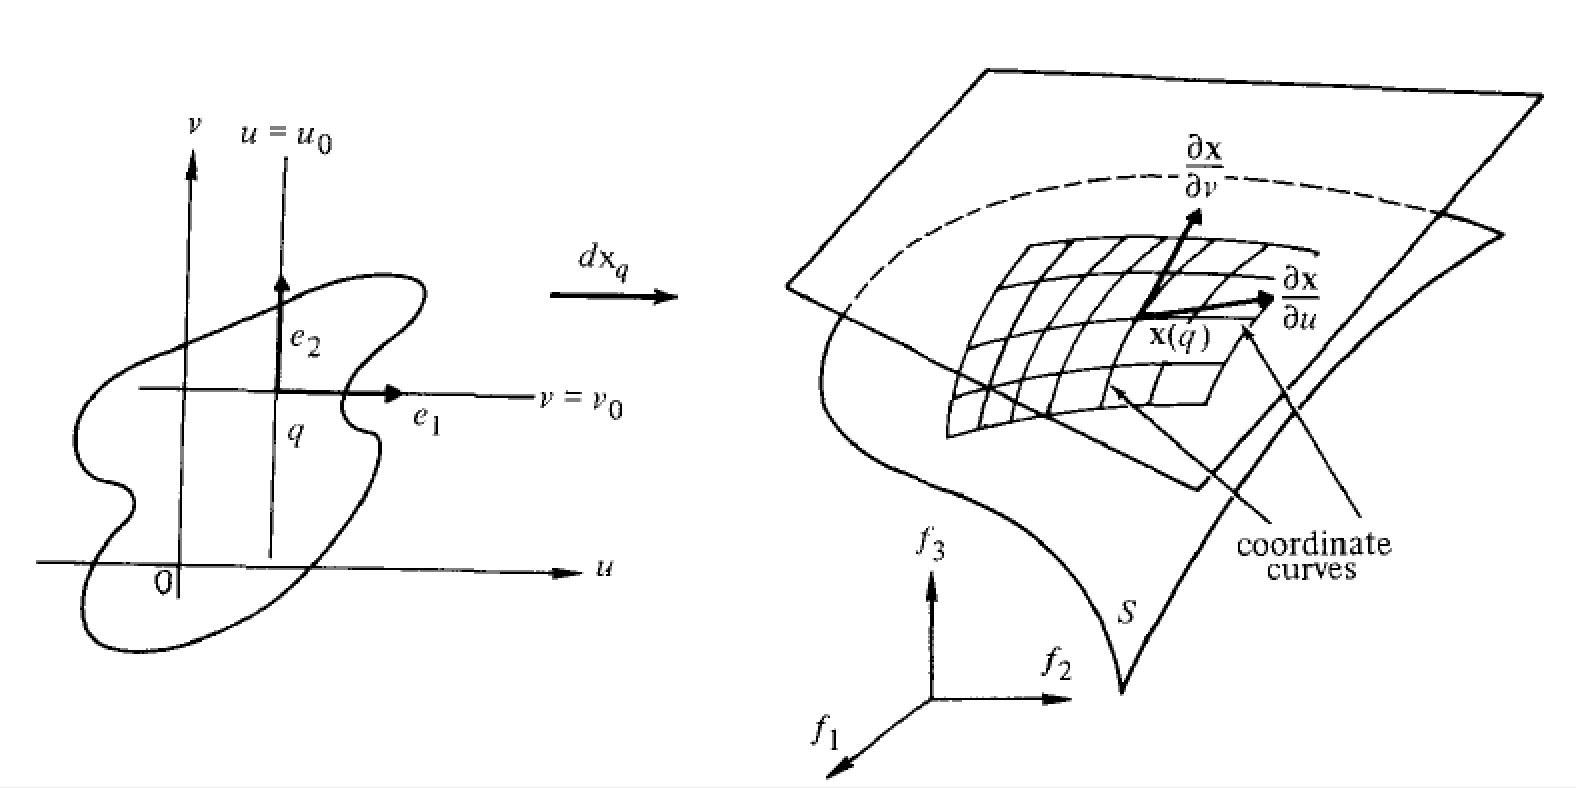
\includegraphics[scale = 0.5]{coordinate_curve.png}}
\end{minipage}
\end{figure}

\item \begin{definition}
 Given a differentiable map $F: U\subset \bR^{n} \rightarrow \bR^{m}$, a point $p\in U$ is a \emph{critical point} of $F$ if $dF_{p}$ is not surjective, i.e. $\partdiff{F}{(\xi_{1}, \ldots, \xi_{m})} = \mb{0}$. The image of critical point is a \emph{critical value}. The value $r$ that is not a critical value is called \emph{regular value} of $F$. Note $dF_{q} \neq 0$ for all $q\in F^{-1}(r)$.
 \end{definition} 

\item Note that for $p$ in a regular surface $\cS$ and let one associated parameterization $\mb{x}$ that is smooth with one-to-one differential, then $\mb{x}$ is a homeomorphism. 

\item $f: V\subset \cS \rightarrow \bR$ is differentiable at $p\in V$ $\Leftrightarrow$ $f\circ \mb{x}: U\subset \bR^{2} \rightarrow \bR$ is differentiable at $\mb{x}^{-1}(p)$.

\item  \begin{definition}
A map $\phi: \cS_{1} \rightarrow \cS_{2}$ is a diffeomorphism if $\phi$ is a smooth map and $\phi^{-1}$ is smooth as well. \\[10pt]
\end{definition} 

\begin{figure}[htb]
\centering
\begin{minipage}{0.6\linewidth}
 \centerline{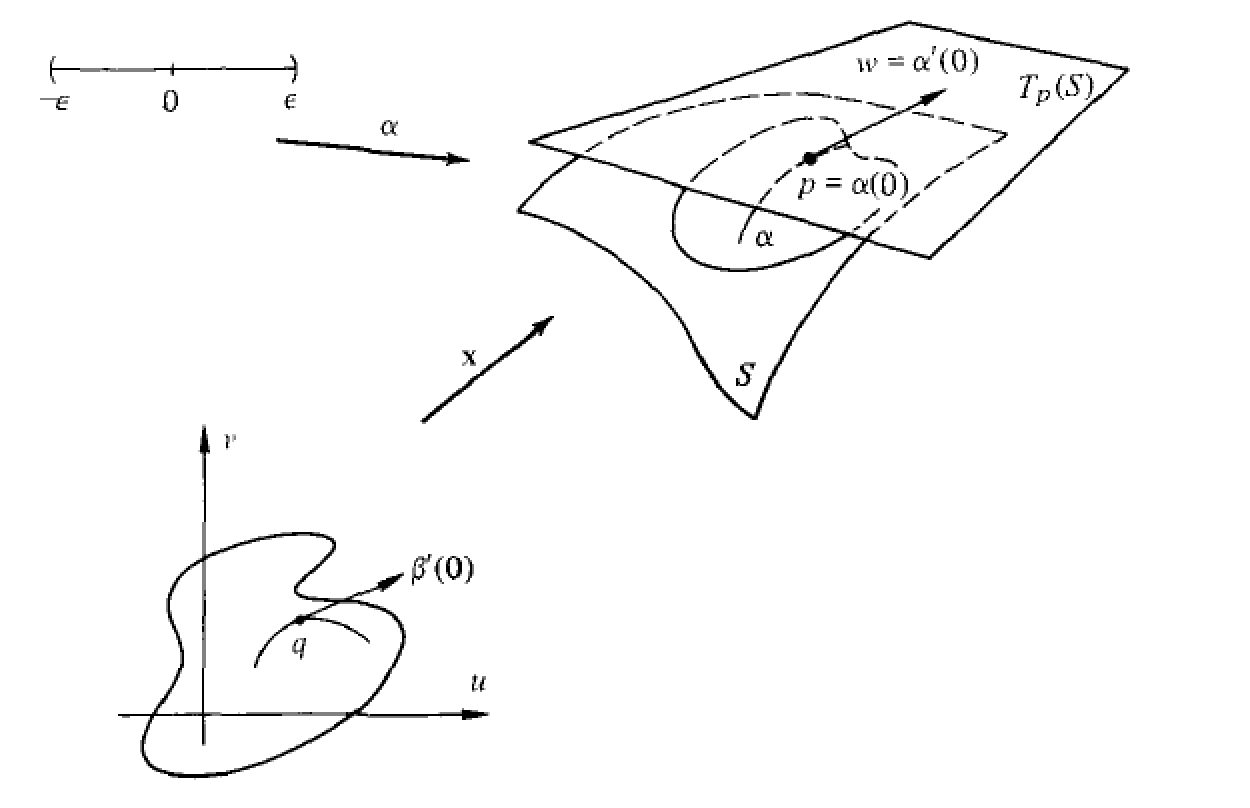
\includegraphics[scale = 0.5]{tangent_plane.png}}
\end{minipage}
\caption{\scriptsize
\textbf{The tangent plane as the subspace of tangent vector of embedded curves. Find the coordinate of the tangent vector in tangent space.}}
\end{figure}

\item  \begin{definition}
The \emph{tangent vector} to a regular surface $\cS$ at $p$ is the tangent vector $\alpha'(0)$ of a differentiable parameterized curve $\alpha: I = (-\epsilon, \epsilon)\rightarrow \cS$ on $\cS$ with $\alpha(0)  = p$. 

 The \emph{tangent plane} to $\cS$ at $p$ consists of all tangent vector $\alpha'(0)$ for all differentiable parameterized curve $\alpha$ on $\cS$ that pass through $p\in \cS$. Denote the tangent space at $p\in \cS$ as $T_{p}S$
\end{definition} 

\item By proposition \ref{prop: tang_param}, the tangent space at $T_{p}S$ has basis $(\partdiff{\mb{x}}{u}(p), \partdiff{\mb{x}}{v}(p)) \equiv (\partdiff{}{u}(p), \partdiff{}{v}(p))$ \citep{amari2007methods}. The tangent space $T_{p}S$ does not depend on the parameterization. 




\item The \emph{differential} of a map $\varphi: V\subset \cS_{1} \rightarrow \cS_{2}$ at $p\in \cS_{1}$ is a linear map $d\varphi_{p}: T_{p}S_{1} \rightarrow T_{\varphi(p)}S_{2}$, where $d\varphi_{p}(\mb{w}) = \beta'(0)$ for $\mb{w}\in T_{p}S_{1}$ with the curve on $\cS_{2}$ as $\beta = \varphi\circ \alpha$ and $\alpha: (-\epsilon, \epsilon) \rightarrow V$ is the curve on $\cS_{1}$. 



\item  \begin{definition}
 A map $\varphi: U\subset \cS_{1} \rightarrow \cS_{2}$ is a \emph{local diffeomorphism} at $p\in U$ if there exists a neighborhood $V\subset U$ of $p$ such that $\phi$ restricted on $V$ is a diffeomorphism onto an open subset $\varphi(V)\subset \cS_{2}. $ 
 \end{definition} 

\item The (unit)  vectors that are normal to the tangent plane at $p$ is called \emph{the (unit) normal vectors} at $p$, denoted as $N(p)$.  It can be defined by the rule
\begin{align*}
N(p) &= \frac{\mb{x}_{u} \wedge \mb{x}_{v}}{\abs{\mb{x}_{u} \wedge \mb{x}_{v}}}(p)
\end{align*}

%\item The angle between two surfaces $\cS_{1}$ and $\cS_{2}$ at the intersecting point $p$ is defined as the angle btw two tangent plane at $p$ or the angle btw the normal vectors at $p$.\\[5pt]

\item  The inner product $\inn{\cdot}{\cdot}$ on the tangent space $T_{p}S$ is induced from $\bR^{3}$. 

\item   \begin{definition}
The \emph{first fundamental form} of a regular surface $\cS\subset \bR^{3}$ at $p\in \cS$ is defined as a  quadratic form,  $I_{p}: T_{p}S \rightarrow \bR$ given by 
\begin{align*}
I_{p}(\mb{w}) &= \inn{w}{w}_{p} = \norm{w}{2}^{2} \ge 0\; \; \mb{w}\in T_{p}S.
\end{align*}
 \end{definition} 
%\item For orthogonal basis $\set{\mb{x}_{u}, \mb{x}_{v}}$, the first fundamental form is the Pythagorean theorem in $\cS$.  
\end{itemize}


\subsection{Normal vector field and the Gauss map}
\begin{itemize}
\item  \begin{definition}
A \emph{(unit) normal vector field} in a neighborhood $U$ associate each point $p\in U\subset \cS$ the unit normal vector $N(p)$ at $p$ that is normal to the tangent space $T_{p}S$.

Given a parameterization $\mb{x}: U\subset \bR^{2} \rightarrow \cS$, the normal vector $N(p)$ at $p$ is given via
\begin{align*}
N(p) &= \frac{\mb{x}_{u} \wedge \mb{x}_{v}}{\abs{\mb{x}_{u} \wedge \mb{x}_{v}}}(p)
\end{align*}

If $V\subset \cS$ is an open subset in $\cS$ and $N: V\rightarrow \bR^{3}$ is a \emph{differentiable} map. It is called a \emph{differentiable field of unit normal vectors} on $V$.

\begin{figure}[thb]
\centering
\begin{minipage}{0.5\linewidth}
 \centerline{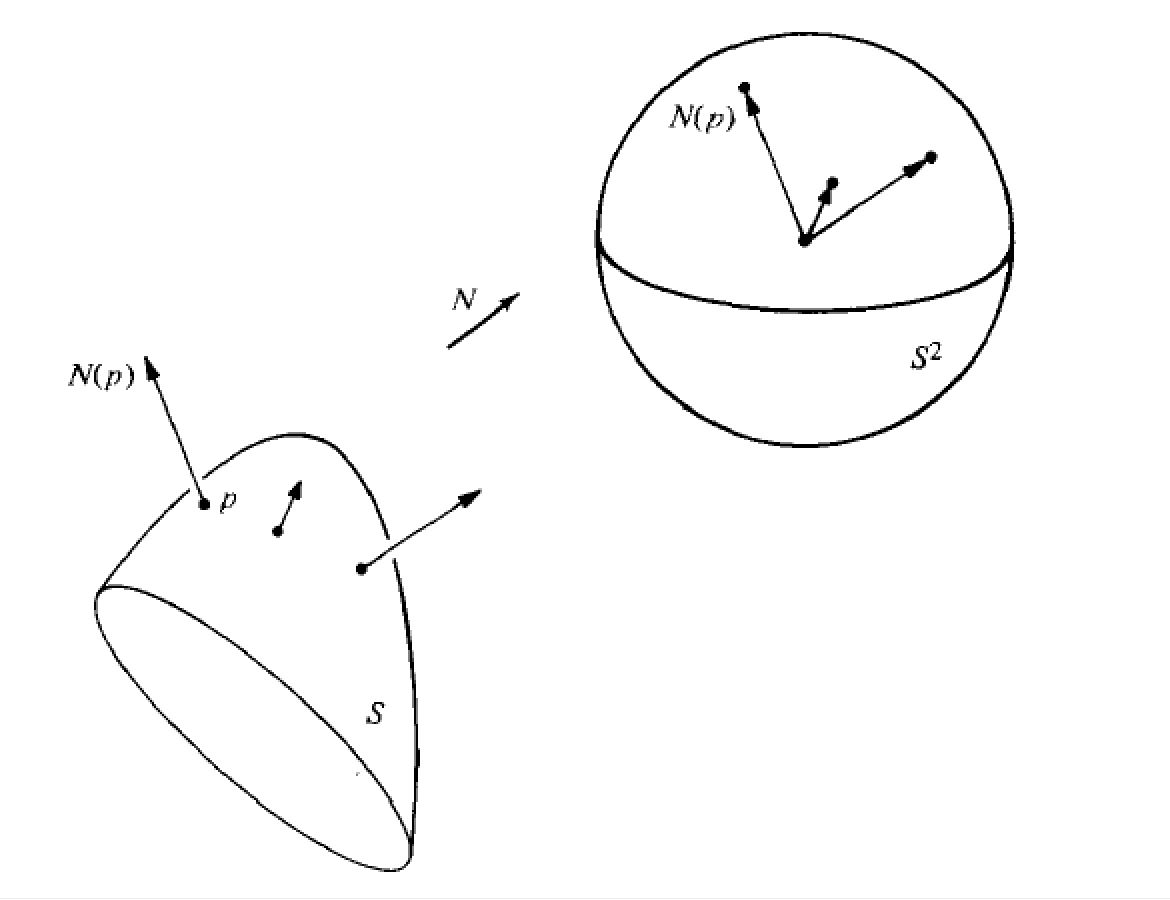
\includegraphics[scale = 0.5]{gauss_map.png}}
\end{minipage}
\caption{\scriptsize
\textbf{The Gauss map from the surface to the unit sphere.}}
\end{figure}
 \end{definition} 

\item The normal vector field may not be well-defined for the whole surface. 
 \begin{definition}
A regular surface is \emph{orientable} if it admits a differentiable  field  of unit normal vectors defined on the whole surface. In terms of this, the choice of such a field $N$ is called an \emph{orientation} of $\cS$. Note that every surface is locally orientable, thus the orientation is a global property. 

 An orientation $N$ induces an orientation on $T_{p}S$, i.e. the basis $\set{v,w}$ is \emph{positive}, if $\inn{v\wedge w}{N}>0.$ The set of positive basis in $T_{p}S$ defines an orientation of the tangent space. 
  \end{definition} 
 
 \item Let $\cS\subset \bR^{3}$ be a surface with an orientation $N$. The map $N: \cS \rightarrow \bR^{3}$ takes its value in the unit sphere $\bS^{2}\equiv \set{(x,y,z)\in \bR^{3}|\;  x^{2}+ y^{2}+ z^{2} =1 }$.  
 \begin{definition}
 The map $N: \cS \rightarrow \bS^{2}$ is called the \emph{Gauss map} of $\cS$.\\
\end{definition} 


 
\item $N$ is differentiable and $dN_{p}: T_{p}S \rightarrow T_{N(p)}\bS^{2}$ is a linear map. Note that $T_{p}S$ and $T_{N(p)}\bS^{2}$ are parallel to each other, so $dN_{p}: T_{p}S \rightarrow T_{p}S$ is a linear transformation in $T_{p}S$.
 



\item \begin{definition}
 %By proposition \ref{prop: Gauss_selfadj}, we can associate $dN_{p}$ with a quadratic form $Q$ in $T_{p}S$ as $Q(\mb{v}) = \inn{dN_{p}(\mb{v})}{\mb{v}}$ for $\mb{v}\in T_{p}S$.
The quadratic form $\Pi_{p}$ defined in $T_{p}S$ by $\Pi_{p}(\mb{v}) = -\inn{dN_{p}(\mb{v})}{\mb{v}}$ is called the \emph{second fundamental form} of $\cS$ at $p$.
\end{definition} 

\item \begin{definition}
%To explore the geometric interpretation of $\Pi_{p}$, we first d
(The \emph{normal curvature} of a regular curve $\cC$ on a regular surface $\cS$ passing through a point $p\in \cC \subset \cS$. )\\
For $\cC \subset \cS$ as a regular curve passing through $p\in \cS$, let $k$ be the curvature of $\cC$ at $p$ and $\cos(\theta) = \inn{\mb{n}}{N}$, where $\mb{n}$ is the normal vector of the curve $\cC$ and $N$ is the normal vector of the surface $\cS$ at $p$. Define $k_{n} = k\cos(\theta)$ as the \emph{orthogonal component} of the \emph{acceleration} vector $\alpha''(s)= k\,\mb{n}$ along the \emph{direction} of normal vector $N(p)$ to the tangent plane of the surface. The quantity $k_{n}$ is referred as the \emph{normal curvature} of a regular curve $\cC$ at a regular surface $\cS$. 
\end{definition} 
\begin{figure}[thb]
\centering
\begin{minipage}{0.6\linewidth}
 \centerline{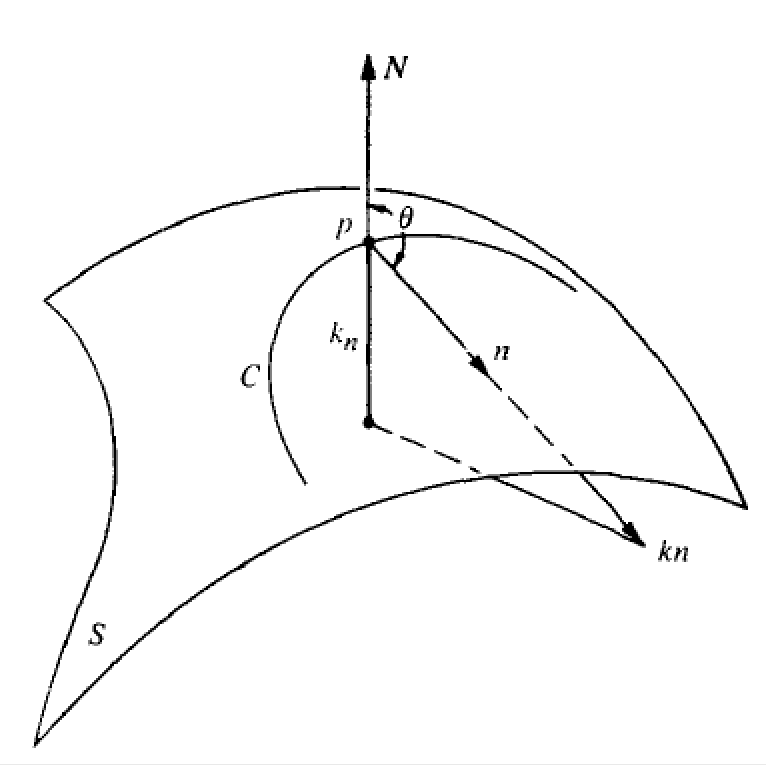
\includegraphics[scale = 0.43]{normal_curv.png}}
\end{minipage}
\caption{\scriptsize
\textbf{The normal curvature $k_{n}$ obtained by projection of $k\mb{n}$ the normal direction of curve $\cC$ to the direction of $N$, the normal direction to the tangent plane of $\cS$. }}
\end{figure}

\item \begin{remark}
By theorem \ref{th: meusnier}, the normal curvature $k_{n}(p)$ is denoted as the normal curvature \emph{along a given direction} at $p$. 

The normal curvature measures the orthogonal component of the curvature of an embedded curve $\cC$ on $\cS$ with respect to the tangent plane of the surface. It measures how rapidly the curve pull away from the \emph{entire tangent space}, as opposed to the original curvature that only measures the strength of the curve to deviate from a \emph{single tangent vector} along the curve in the tangent space. 

It is determined by the angle between the osculating plane of the curve $\cC$ and the tangent plane of the surface $\cS$ at the intersecting point $p\in \cS$. Note that $\mb{t}$ for the curve lies in both the osculating plane of the curve $\cC$ and the tangent plane of the surface $\cS$.\\
\end{remark}

\item   \begin{remark}
The second fundamental form $\Pi_{p}(\mb{v})$ for any unit vector $\mb{v}\in T_{p}S$ is the \emph{normal curvature} of the $\cC$ passing through $p$ with $\alpha'(0) = \mb{v}$.

In fact, the second fundamental form is the component of the \emph{second derivative} of parameterization $\mb{x}(u(t), v(t))$ \emph{perpendicular} to the tangent plane of $\cS$.
\end{remark}

\item \begin{definition} 
The intersection of $\cS$ with the plane containing the unit vector $\mb{v}\in T_{p}S$ and $N(p)$ is called the \emph{normal section} of $\cS$ at $p$ along $\mb{v}$. It is a plane curve with normal vector $\mb{n} = \pm N(p)$ or $0$. Its curvature is the absolute value of the normal curvature at $p$ along $\mb{v}$. 

Theorem \ref{th: meusnier} states that \emph{the absolute value of the normal curvature }at $p$ of a curve $\alpha(s)$ is equal to \emph{the curvature of the normal section} of $\cS$ at $p$ along $\alpha'(0)$.\\
\end{definition}

\item  \begin{remark}
If the surface is a plane, then all normal vectors are straight lines; hence, the  osculating plane of the curve $\cC$ and the tangent plane of the surface $\cS$ coincides and the normal curvature is zero. In terms of this, $dN_{p} \equiv 0$ for all $p$.
\end{remark}

\item  \begin{remark}
 For plane and sphere, all directions at all points are principal directions and the normal curvature are constant, i.e. the second fundamental form at every point, restricted to the unit vectors, is constant. For $\Pi_{p}(\mb{v}) = 0$ for all $p\in \cS$ and all $\norm{\mb{v}}{} = 1$, it is a plane, whereas  $\Pi_{p}(\mb{v}) = c$ for all $p\in \cS$ and all $\norm{\mb{v}}{} = 1$, it is a sphere with radius $1/c$. All directions are extremals for the normal curvature. 
 \end{remark}

\item  \begin{definition} 
If a regular connected curve $\cC$ on $\cS$ is such that for every $p\in \cC$, the tangent line of $C$ is principal direction of surface at $p$, then $\cC$ is said to be a \emph{line of curvature of} $\cS$
\end{definition}


\item \begin{remark} It is clear that the necessary and sufficient condition for a curve $\alpha(t)$ to be a line of curvature is that
\begin{align*}
dN_{p}(\alpha'(t)) = N'(t) &= \lambda(t)\alpha'(t), 
\end{align*}where $N(t) = N\circ \alpha(t)$ and $
\lambda(t)$ is differentiable function of $t$ with $-\lambda(t)$ being the principal curvature of surface along $alpha'(t)$.\\
\end{remark}



\item \begin{definition}
The \emph{Gaussian curvature} $\mb{K}$ of $\cS$ at $p$ is defined as $\mb{K}\equiv \det\paren{dN_{p}}$ and the \emph{mean curvature} $\mb{H}$ is defined as $\mb{H}\equiv -\frac{1}{2}\text{trace}\paren{dN_{p}}$. 

Note that $\mb{K} = k_{1}k_{2}$ for $k_{1}, k_{2}$ principal curvatures at $p$ and $\mb{H} = \frac{1}{2}\paren{k_{1}+ k_{2}}$. \end{definition}
%\\[10pt]

%\item A point $p$ of a surface $\cS$ is called
%\begin{itemize}
%\item Elliptic, if $\mb{K}= \det\paren{dN_{p}} >0$; 
%\item Hyperbolic, if $\mb{K}=\det\paren{dN_{p}} <0$;
%\item Parabolic, if  $\mb{K}=\det\paren{dN_{p}} =0$ but $dN_{p}\neq 0$;
%\item Planar, if $dN_{p} = 0$.
%\end{itemize}
%
%\item All curves passing through an \emph{elliptic} point $p$ have their normal vector pointing towards the same side of the tangent plane. The principal curvatures are of the same sign and the Gaussian curvature is positive. 
%
%\item There are curves passing through an \emph{hyperbolic} point $p$ to have their normal vector pointing towards the any of the sides of the tangent plane. The principal curvatures are of the opposite sign and the Gaussian curvature is negative. 
%
%\item At \emph{parabolic} point $p$, the Gaussian curvature is zero, but one of the principal curvature is nonzero. The points of a cylinder, e.g., are parabolic points. 
%
%\item At a \emph{planar} point, all principal curvatures are zero. The points in a plane satisfies this condition. An nontrival planer point, e.g. is the $(0,0,0)$ for the surface of revolution obtained by rotating the curve $z= y^{4}$ along the $z$-axis.   
%
%\item If at $p$, the principal curvatures are the same $k_{1} = k_{2}$, this point is called an \emph{umbilical point} of $\cS$; in particular, the planar points $k_{1}=k_{2} = 0$ are umbilical points. \citep{do1976differential}
%
%If all points of a connected surface $\cS$ are umbilical points, then $\cS$ is either a plane or a sphere.\\
%
% \item Let $p\in \cS$. An \emph{asymptotic direction} of $\cS$ at $p$ is a direction in $T_{p}S$ for which the normal curvature is zero. 
% 
% An \emph{asymptotic curve} of $\cS$ is a regular connected curve $\cC\subset \cS$ such that for each $p\in \cC$ the tangent line of $\cC$ at $p$ is an asymptotic direction. 
% 
% It is clear that at elliptic point, there is no asymptotic directions. 
 
% \item For $p\in \cS$, the \emph{Dupin indicatrix} at $p$ is the set of vectors $\mb{w}$ of $T_{p}S$ such that $\Pi_{p}(\mb{w}) = \pm 1$.
 
%\item At a point $p\in \cS$, two nonzero vectors $\mb{w}_{1}$ and $\mb{w}_{2}$ in $T_{p}S$ are \emph{conjugate}, if $\inn{dN_{p}(\mb{w}_{1})}{\mb{w}_{2}} = \inn{\mb{w}_{1}}{dN_{p(\mb{w}_{2})}} = 0$. Two directions $\mb{r}_{1}$ and $\mb{r}_{2}$ at $p$ are conjugate if a pair of nonzero vectors  $\mb{w}_{1}$ and $\mb{w}_{2}$ parallel to $\mb{r}_{1}$ and $\mb{r}_{2}$, respectively, are conjugate. 

%Note that all principal directions are conjugate. The asymptotic directions are conjugate to itself. At a nonplanar umbilic, every pair of orthogonal directions are conjugate directions and at a planar umbilic, any two directions are conjugate. 
%
%For $p\in \cS$, and the basis $\set{\mb{e}_{1}, \mb{e}_{2}}$ are basis of $T_{p}S$ given by the principal directions. Let $\theta$ and $\varphi$ be the angles that a pair of directions $\mb{r}_{1}$ and $\mb{r}_{2}$ make with $\mb{e}_{1}$. Then two directions $\mb{r}_{1}$ and $\mb{r}_{2}$ are conjugate iff 
%\begin{align*}
%k_{1}\cos(\theta)\cos(\varphi) &= - k_{2}\sin(\theta)\sin(\varphi)
%\end{align*}
%
%For elliptic (or hyperbolic) points, the conjugate direction can be constructed using Dupin indicatrix at $p$. For given direction $\mb{r}_{1}$, we construct a straight line with $\mb{r}_{1}$ direction going through the origin of $T_{p}S$. Then we find the intersection point of $\mb{r}_{1}$ with the Dupin indicatrix $\set{(\xi, \eta)\;| \;\;k_{1}\xi^{2} + k_{2}\eta^{2} = 1}$ as $q_{1}, q_{2}$. The tangent line of the Dupin indicatrix at these two points are parallel lines with common direction $\mb{r}_{2}$ that is conjugate to $\mb{r}_{1}$.
\end{itemize}

\subsection{The intrinsic geometry of surfaces}
\begin{itemize}
\item   \begin{definition}
For two regular surfaces $\cS$ and $\cS'$, a diffeomorphism $\varphi: \cS \rightarrow \bar{\cS}$ is an \emph{isometry} if for all $p\in \cS$ and all pairs $\mb{w}_{1}, \mb{w}_{2} \in T_{p}S$ we have
\begin{align*}
\inn{\mb{w}_{1}}{\mb{w}_{2}}_{p} &= \inn{d\varphi_{p}(\mb{w}_{1})}{d\varphi_{p}(\mb{w}_{2})}_{\varphi(p)}.
\end{align*} 
The surface $\cS$ and $\bar{\cS}$ are said to be \emph{isometric}. 
\end{definition}

\item \begin{remark}
 The diffeomorphism $\varphi$ is an isometry if the differential $d\varphi$ it preserves the inner product. It follows that the first fundamental form 
\begin{align*}
I_{p}(\mb{w}) &= \inn{w}{w}_{p} = \inn{d\varphi_{p}(\mb{w})}{d\varphi_{p}(\mb{w})}_{\varphi(p)} = I_{\varphi(p)}(d\varphi_{p}(\mb{w})),\quad \forall\,\mb{w}\in T_{p}S.
\end{align*}  Conversely, if the differential of a diffeomorphism preserves the first fundamental form, it is an isometry. 
\end{remark}

\item \begin{definition}
 A map $\varphi: V \rightarrow \bar{\cS}$ of a neighborhood $V$ of $p\in \cS$ is a \emph{local isometry} at $p$ if there exists a neighborhood $\bar{V}$ of $\varphi(p) \in \bar{\cS}$ such that $\varphi: V \rightarrow \bar{V}$ is an isometry.  If there exists a local isometry into $\bar{\cS}$ at every $p\in \cS$, the surface $\cS$ is said to be \emph{locally isometric} to $\bar{\cS}$. Then $\cS$ and $\bar{\cS}$ are \emph{locally isometric} if $\cS$ is locally isometric to $\bar{\cS}$ and $\bar{\cS}$ is locally isometric to $\cS$. 
 \end{definition}



\item \begin{definition} 
Given the first fundamental form, the \emph{intrinsic distance} between two points on the surface can be defined as the infimum of the arc length between these points. This distance is invariant under isometry, i.e. $\varphi: \cS \rightarrow \bar{\cS}$ is an isometry, then $d(p,q) = d(\varphi(p), \varphi(q)),\; p,q\in \cS$.
\end{definition}

\item  \begin{remark}
The notion of isometry is a natural concept of equivalence for the metric properties of regular surface. Similarly, the notion of diffeomorphism is an equivalence relationship form the point of view of differentiability. 

Note that for a diffeomorphism $\varphi$ that is a local isometry for every $p\in \cS$, then $\varphi$ is a (global) isometry. 

It is possible that two surfaces are locally isometric but are not \emph{globally isometric}, e.g. the plane and the cylinder. \\
\end{remark}

\item Given a parameterization $\mb{x}: U\rightarrow \cS$ in the orientation of a regular surface $\cS$, it is possible to assign a natural trihedron $(\mb{x}_{u}, \mb{x}_{v}, N)$ at each point $p\in \mb{x}(U)$. 

\begin{definition}  The linear coefficients of the second partial derivatives of the parameterization $(\mb{x}_{uu}, \mb{x}_{uv}, \mb{x}_{vv})$ under the basis vectors $(\mb{x}_{u}, \mb{x}_{v})$ at $p$ is referred as the \emph{Christoffel symbol}, $\Gamma_{i,j}^{k}$, where the upper index $k=1,2$ is related to the basis vector $(\mb{x}_{u}, \mb{x}_{v})$, and the lower index $(i,j) \in \set{1,2}\times \set{1,2}$ is related to the intrinsic parameter $(u,v)$ under second order partial derivatives. 
\end{definition}

%Note that  $(\mb{x}_{uu}, \mb{x}_{uv}, \mb{x}_{vv})$ is seen also as the partial derivative of the basis vector $(\mb{x}_{u}, \mb{x}_{v})$. Thus the Christoffel symbol is the linear coefficient in representing  the partial derivative of the basis vector $(\mb{x}_{u}, \mb{x}_{v})$ under these basis vectors itself. 

\item   \begin{remark}
The Christoffel symbols $\Gamma_{i,j}^{k},\; i,j,k=1,2$ are uniquely determined via the coefficients of first fundamental form $(E,F,G)$. 

\emph{All geometric concepts and properties expressed in terms of Christoffel symbols are invariant under isometries}.
\end{remark}

\item  \begin{remark}
 In THEOREMA EGREGIUM (theorem \ref{th: Gauss_theorem}) by Gauss,  it shows that the Gaussian curvature $\mb{K}$ of a surface is invariant by local isometries. 

It is noted that in essence, the definition of the Gaussian curvature make use of the position of the surface in the space. However, the Gaussian theorem shows that it only depends on the metric structure (i.e. the first fundamental form) of the surface not on the position of the surface in the ambient space. 
\end{remark}

\item  \begin{remark}
The \emph{compatibility equations} (i.e. the \emph{Gauss formula} and \emph{Mainardi-Codazzi equations}) is a system of differential equations for the coefficients of the first and the second fundamental forms ($E,F,G,e,f,g$) and also there is no further relations btw these coefficients.
\end{remark}

\item  \begin{remark}
In Bonnet theorem \ref{th: Bonnet_th}, it shows that the coefficients of the first and the second fundamental forms ($E,F,G,e,f,g$) uniquely determines the parameterization of the surface locally up to a rigid transformation. That is, these coefficients are sufficient to determine the local structure of a surface.  
\end{remark}

%\item A summary of the coefficients for the first and second fundamental form
%\begin{align}
%E(u,v) &= \inn{\mb{x}_{u}}{\mb{x}_{u}} \nonumber\\
%F(u,v) &= \inn{\mb{x}_{u}}{\mb{x}_{v}} \nonumber\\
%G(u,v) &= \inn{\mb{x}_{v}}{\mb{x}_{v}} \nonumber \\
%e(u,v)  &=  - \inn{N_{u}}{\mb{x}_{u}} = \inn{N}{\mb{x}_{uu}} \nonumber\\
%f(u, v)&= - \inn{N_{u}}{\mb{x}_{v}} =  \inn{N}{\mb{x}_{vu}} =  \inn{N}{\mb{x}_{uv}} =  -\inn{N_{v}}{\mb{x}_{u}}\nonumber\\
%g(u, v)&=   - \inn{N_{v}}{\mb{x}_{v}} = \inn{N}{\mb{x}_{vv}} \label{eqn: coeff_first_sec_fund_form}
%\end{align}
\end{itemize}

\subsection{Parallel transport and geodesic}
\begin{itemize}
\item  \begin{definition}
A \emph{(tangent) vector field} $\mb{w}$ in an open set $U \subset \cS$ of a regular surface $\cS$ is a correspondence which assigns to each $p\in U$ a vector $\mb{w}(p) \in T_{p}S$. The vector field $\mb{w}$ is \emph{differentiable} at $p\in U$ if, for some parameterization $\mb{x}(u,v)$ at $p$, the functions $a(u,v)$ and $b(u,v)$ given by 
\begin{align*}
\mb{w}(p) &= a(u,v)\mb{x}_{u} + b(u,v)\mb{x}_{v}
\end{align*}
are differentiable functions at $p$; it is clear that this definition does not depends on the choice of $\mb{x}$. 
\end{definition}


\item Let $\mb{w}$ be a differentiable vector field in an open subset $U \subset \cS$ and $p\in U$, i.e. $\mb{w}(p) \in T_{p}S$. Let $\mb{y}\in T_{p}S$. Consider a parameterized curve $\alpha: (-\epsilon, \epsilon) \rightarrow U$, with $\alpha(0) = p$ and $\alpha'(0) = \mb{y}$, and let $\mb{w}(t), t\in (-\epsilon, \epsilon)$, be the restriction of the vector field to the curve $\alpha$. \begin{definition}
The vector obtained by the normal projection of $\frac{d\mb{w}}{dt}(0)$ onto the plane $T_{p}S$ is called the \emph{covariant derivative at $p$ of the vector field $\mb{w}$ relative to the vector $\mb{y}$.} This covariant derivative is denoted by $\frac{D\mb{w}}{dt}(0)$ or $D_{\mb{y}}\mb{w}.$
\end{definition}

\begin{figure}[thb]
\centering
\begin{minipage}{0.6\linewidth}
 \centerline{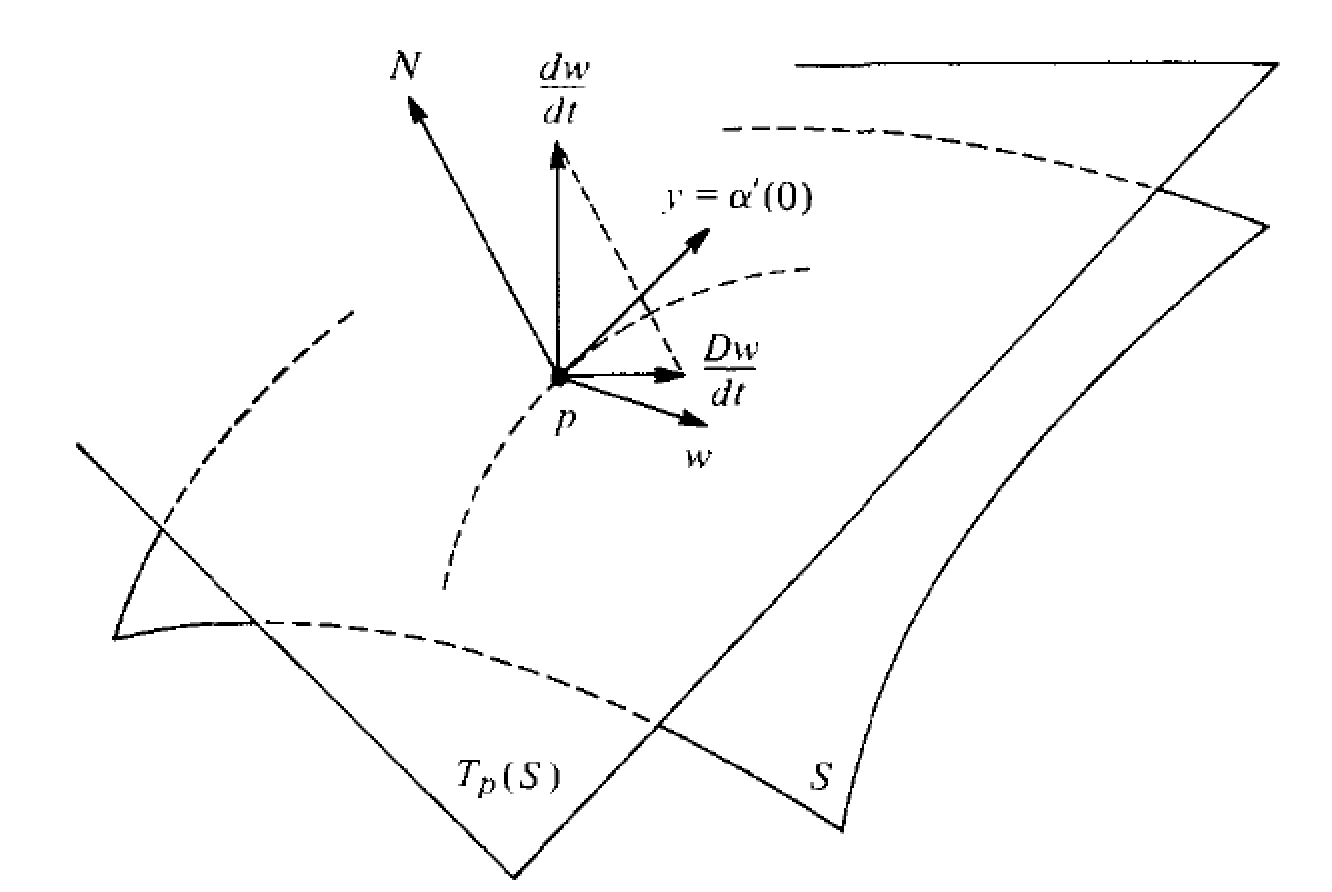
\includegraphics[scale = 0.43]{cov_deriv.png}}
\end{minipage}
\caption{\scriptsize
\textbf{The covariant derivative $\frac{D\mb{w}}{dt}$ at $p$ relative to vector $\mb{y}$, given by projection of Euclidean derivative $\frac{d\mb{w}}{dt}$ along the curve $\alpha$ with $\alpha' = \mb{y}$ onto the tangent plane of the surface. }}
\end{figure}

\item \begin{remark}
Note that the concept of covariant derivative makes use of normal vector of $\cS$ and the curve $\alpha$ tangent to $\mb{y}$ at $p$. Its concern is the rate of change of the vector field along a curve. 

The concept of the covariant derivative generalize the usual definition of the Euclidean derivative as it take into account the change of the basis vector of the tangent plane along the curve on the surface $\cS$ and only consider its tangential projection. 

For the differential of a vector field on Euclidean space, the basis of the tangent plane is defined universally and they remain unchanged when moving on the plane, whereas only the component of the differential on each axis changes, i.e.
\begin{align*}
\frac{d\mb{w}}{dt} &= a'\mb{x}_{u} + b'\mb{x}_{v}.
\end{align*} However, when moving on the surface, given that these components of the differential are unchanged, since the axis is locally defined, it will change when points moves, and it will cause the change of the differential vector field, i.e. the differential of a vector field on the surface, 
\begin{align*}
\frac{d\mb{w}}{dt} &= a'\mb{x}_{u} + b'\mb{x}_{v} + a\paren{\mb{x}_{uu}u' + \mb{x}_{uv}v'} + b\paren{\mb{x}_{vu}u' + \mb{x}_{vv}v'}. 
\end{align*} And the covariant derivative is given by 
\begin{align*}
\frac{D\mb{w}}{dt} &= \mathcal{P}_{T_{p}S}\paren{\frac{d\mb{w}}{dt} }.
\end{align*}
\end{remark}


\item A parameterized curve $\alpha: [0, l] \rightarrow \cS$ is the restriction to $[0,l]$ of a differentiable mapping of $(0-\epsilon, l+\epsilon), \epsilon>0$ into $\cS$. If $\alpha(0) = 0, \alpha(l) = q$, we say that $\alpha$ \emph{joins} $p$ to $q$. $\alpha$ is regular if $\alpha'(t)\neq 0, \;t\in [0,l]$.

\item Denote $I= [0,l]$. Let $\alpha: I\rightarrow \cS $ be a parameterized curve in $\cS$.   \begin{definition}
A \emph{vector field $\mb{w}$ along $\alpha$} is a correspondence that assigns to each $t\in I$ a vector 
\begin{align*}
\mb{w}(t) \in T_{\alpha(t)}\cS.
\end{align*}
The vector field is \emph{differentiable} at $t_{0}\in I$ if for some parameterization $\mb{x}(u,v)$ in $\alpha(t_{0})$ the components $a(t), b(t)$ of $\mb{w}(t) = a\mb{x}_{u} + b\mb{x}_{v}$ are differentiable functions of $t$ at $t_{0}$. $\mb{w}$ is \emph{differentiable} in $I$ if it is differentiable for every $t\in I$.
\end{definition}


\item \begin{definition}
A vector field $\mb{w}$ along a parameterized curve $\alpha: I \rightarrow \cS$ is said to be \emph{parallel} if $\frac{D\mb{w}}{dt} = 0$ for every $t\in I$.  
\end{definition}

\item \begin{remark} If the surface is plane, then the tangent vector field is constant along any curve; that is, the angle with a fixed direction and the length of the vector are constant. 

A straight line a the plane is seen as parallel transport of the tangent vector $\alpha'$ along the curve of $\alpha$, i.e. the only curve that maintain the direction and length of its tangent line unchanged is the straight line on the plane. 
\end{remark}
\begin{figure}[tbh]
\centering
\begin{minipage}{0.6\linewidth}
 \centerline{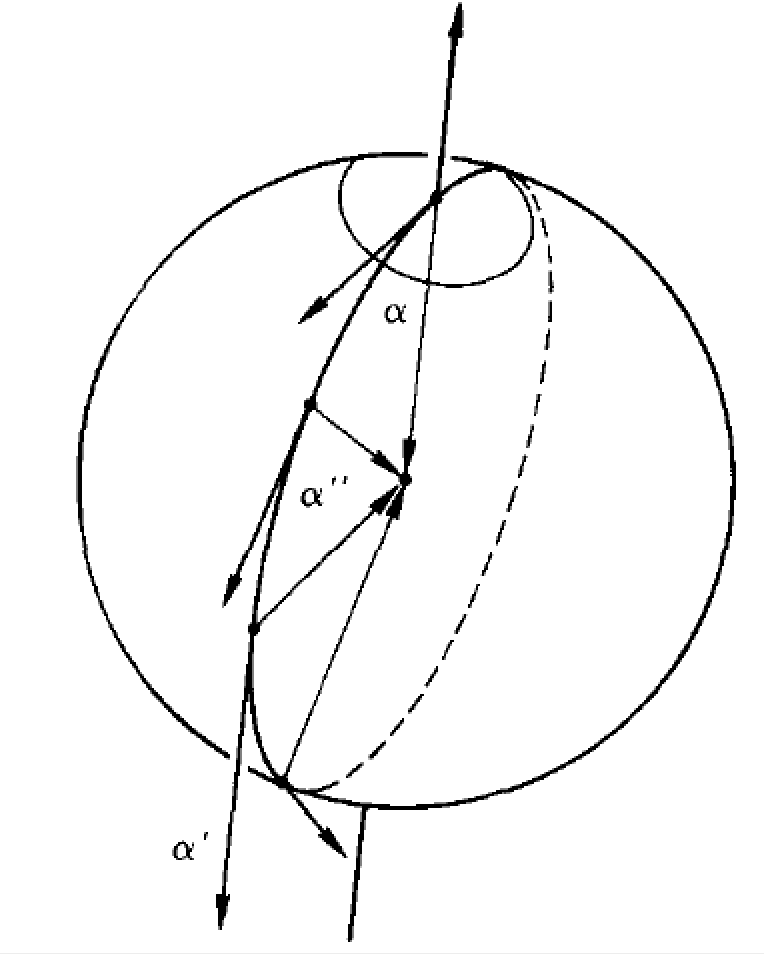
\includegraphics[scale = 0.43]{para_transp.png}}
\end{minipage}
\caption{\scriptsize
\textbf{For the sphere surface, the tangent vector field of any great circle is a parallel field on surface. Note that the differential of the tangent vector is normal to the surface, so its tangential component is zero.  }}
\end{figure}

\item  \begin{remark}
Given a curve on the surface, and an initial vector in tangent space, there exists \emph{unique} vector field that is parallel along this curve. \\
\end{remark}

\item Let $\alpha: I \rightarrow \cS$ be a parameterized curve and $\mb{w}_{0}\in T_{\alpha(t_{0})}S$, $t_{0}\in I$. \begin{definition}
Let $\mb{w}$ be the parallel vector field along $\alpha$, with $\mb{w}(t_{0}) = \mb{w}_{0}.$  The vector $\mb{w}(t_{1}), t_{1}\in I$ is called the \emph{parallel transport} of $\mb{w}(t_{0})= \mb{w}_{0}$ along $\alpha$ at point $t_{1}$. \end{definition}

By using parallel transport, one can find the vector  at new point in vector field from its value at old point along the curve.  

\item \begin{remark}
 Given that the curve $\alpha$ is regular, then the parallel transport does not depends on the parameterization of the curve. As for $\beta: J \rightarrow \cS$ another parameterization for the curve $\alpha(I)$, then 
\begin{align*}
\frac{D\mb{w}}{d\sigma} &= \frac{D\mb{w}}{dt}\frac{dt}{d\sigma}, \forall t\in I, \sigma\in J.
\end{align*}
As $dt/d\sigma\neq 0$ then $\mb{w}(t)$ is parallel iff $\mb{w(\sigma)}$ is parallel. \\
\end{remark}

\item Define the linear mapping $P_{\alpha}: T_{p}(S) \rightarrow T_{q}(S)$ for $p,q\in \alpha$ that assign each $\mb{v}\in  T_{p}(S)$ its parallel transport at $q$ along $\alpha$. Then by Proposition \ref{prop: para_transp}, this map is an \emph{isometry}.

In other word,  \begin{remark} 
the angle of the parallel transport of $\mb{w}$ along $\alpha$ to the tangent line of the curve $\alpha'$ is constant.  
\end{remark}


\item \begin{remark}
This shows a geometric interpretation of the parallel transport.
\begin{figure}[htb]
\centering
\begin{minipage}{0.6\linewidth}
 \centerline{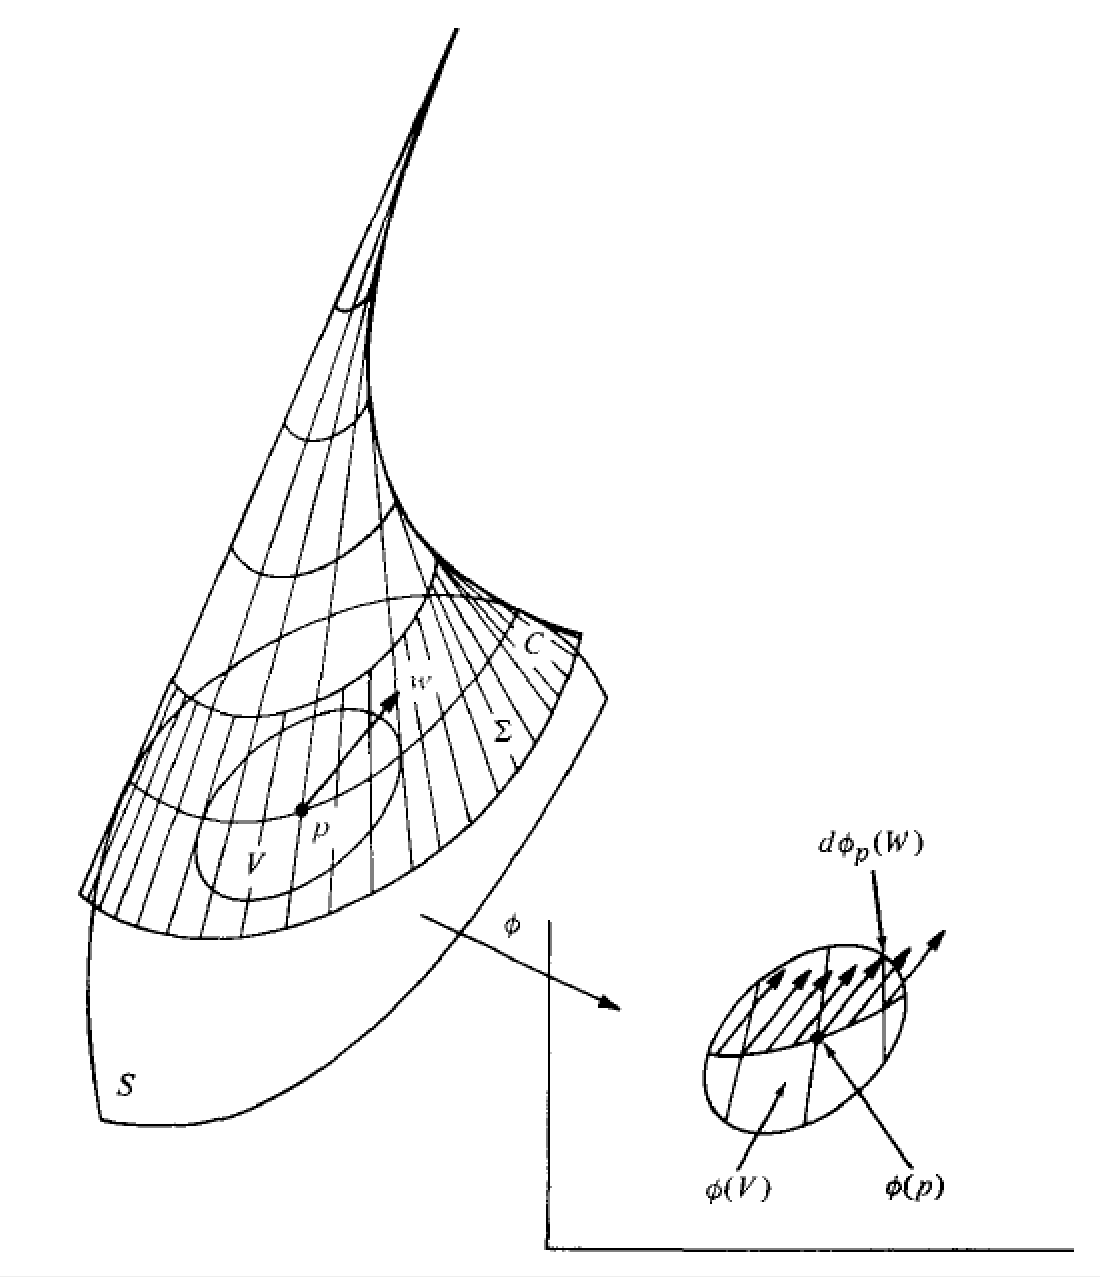
\includegraphics[scale = 0.43]{para_transp3.png}}
\end{minipage}
\caption{\scriptsize
\textbf{The parallel transport on the surface along $\cC$ is equal locally to those on the envelop of tangent plane of $\cC$.  By using the differential of an isometry $\varphi$, we can find a plane on which the parallel lines of the differential mapping $d\varphi(\mb{w})$ is a representation of the parallel transport.   }}
\end{figure}
\end{remark}\vspace{15pt}


 

\item \begin{definition}
 A nonconstant, parameterized curve $\gamma: I \rightarrow \cS$ is said to be \emph{geodesic} at $t\in I$ if the field of its tangent vectors $\gamma'(t)$ is parallel along $\gamma$ at $t$; that is, 
\begin{align*}
\frac{D\gamma'(t)}{dt} = 0;
\end{align*}
$\gamma$ is a \emph{parameterized geodesic} if it is geodesic for all $t\in I$.

It is seen that $\abs{\gamma'(t)} = c\neq 0$ and the geodesic can be reparameterized by its arc length $s$.
\end{definition}

\item \begin{definition}
A regular connected curve $\cC$ in $\cS$ is said to be a \emph{geodesic} if, for every $p\in \cC$, the parameterization $\alpha(s)$ of a coordinate neighborhood of $p$ by arc length $s$ is a \emph{parameterized geodesic}; that is $\alpha'(s)$ is a parallel vector field along $\alpha(s)$.
\end{definition}

\item \begin{remark} Assume the curve $\alpha(t)$ is a motion on $\cS$ with \emph{unit} velocity $\alpha'(t)$. The trajectory of $\alpha(t)$ at a given interval $I$ is a geodesic iff the acceleration vector $\alpha''(t) = k\mb{n}$ is normal to the tangent plane of the surface, or the tangential acceleration is zero. In other word, a regular curve $\cS \subset \cS$ is a geodesic iff its principal normal (, i.e. the line that contains $\mb{n}$ and passes through $\cC$) at each point $p\in \cC$ is parallel to the normal to $\cS$ at $p$.\\
\end{remark}
  
\item Let $\mb{w}$ be a differentiable vector field of \emph{unit} vectors along a parameterized curve $\alpha: I \rightarrow \cS$ on an oriented surface $\cS$. 
\begin{definition}
Since $\mb{w}(t), t\in I$ is a unit vector field, $d\mb{w}(t)/dt$ is normal to $\mb{w}(t)$, and therefore, 
\begin{align*}
\frac{D\mb{w}}{dt} &= \lambda\,\paren{\mb{N} \wedge \mb{w}(t)},
\end{align*} 
where $\lambda = \lambda(t)$ denoted as $\brac{D\mb{w}/dt}$, is called \emph{the algebraic value} of the covariant derivative of $\mb{w}$ at $p$.
\end{definition}

Note that $\lambda = \brac{D\mb{w}/dt} = \inn{d\mb{w}(t)/dt}{\mb{N} \wedge \mb{w}}$ and its sign depends on the orientation of the surface. 

\item  \begin{remark}
The concept of parallel transport and geodesic does not depend on the orientation of the surface. But the geodesic curvature changes its sign with the change of orientation of the surface. 
\end{remark}

\item Let $\cC$ be an oriented regular curve contained on an oriented surface $\cS$, and let $\alpha(s)$ be a parameterization of $\cC$ in a neighborhood of $p\in \cS$, by the arc length $s$. 
\begin{definition}
The algebraic value of the covariant derivative $\brac{D\alpha'(s)/ds} = k_{g}$ at $p$ is called the \emph{geodesic curvature} of $\cC$ at $p$. 
\end{definition}

\item  \begin{remark}
The regular geodesic curve is characterized as the regular curve whose \emph{geodesic curvature is zero}.  

The \emph{absolute value} of the geodesic curvature $k_{g}$ of $\cC$ at $p$ is tangential component of the vector $\alpha''(s)= k\mb{n}$, where $k$ is the curvature of $\cC$ and $\mb{n}$ is the normal vector of the curve $\cC$. Note that the absolute value of its normal component is the absolute value of the normal curvature $k_{n}$. So
\begin{align*}
k^{2} = k_{g}^{2} + k_{n}^{2}.
\end{align*} The absolute value of the geodesic curvature is the same if two surfaces are tangent along the curve. 
\begin{figure}[tbh]
\centering
\begin{minipage}{0.6\linewidth}
 \centerline{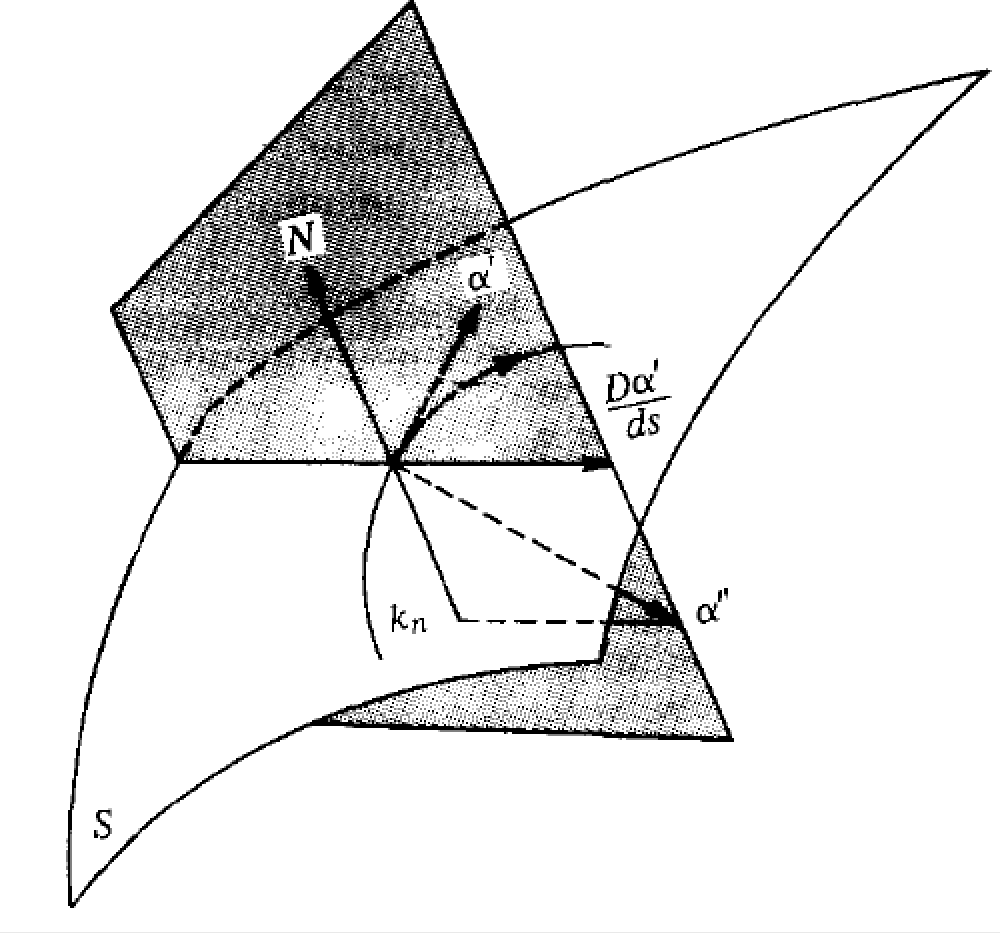
\includegraphics[scale = 0.43]{geo_curv.png}}
\end{minipage}
\caption{\scriptsize
\textbf{The geodesic curvature given by projecting $\alpha''$ to the tangent plane. Its projection on the normal plane is the normal curvature.   }}
\end{figure}
\end{remark}

\item \begin{remark}
The geodesic curvature is the \emph{rate of change of the angle that the tangent to the curve makes with a parallel direction along the curve}. That is, define $\mb{w}, \mb{v}$ be two vector field with unit length $\abs{\mb{w}} = \abs{\mb{v}} = 1$ and a differentiable map $\phi: I \rightarrow \bR$ to be the angle from $\mb{v}(t)$ to $\mb{w}(t)$ in the orientation of the surface. Then 
\begin{align*}
k_{g}(s) &= \brac{\frac{D\alpha'(s)}{ds}} = \frac{d\phi}{ds}.
\end{align*}
For a plane, as the parallel direction is constant, the geodesic curvature becomes the usual curvature. 
\end{remark}
\end{itemize}
\subsection{Functions on manifold}
\begin{itemize}
\item \begin{definition}\citep{lee2003introduction}
Let $\cM$ be a smooth manifold and $T_{p}\cM$ be the tangent space at $p\in \cM$. The \emph{cotangent space} $T^{*}_{p}\cM$ is the dual space of tangent space $T_{p}\cM$, which consists of all linear functionals $\omega$ on $T_{p}\cM$, i.e. $\omega: T_{p}\cM\rightarrow \bR$ and it is called the\emph{ tangent covectors} or \emph{covariant vectors} since its components transform in the same way as the coordinate partial derivatives. 
\end{definition}
Note the tangent vector is referred as \emph{contravariant vectors} since its components transform in the opposite way as the coordinate partial derivatives.  

\item For $T_{p}\cM = \text{span}\set{ \rlat{\partdiff{}{x_{i}}}{p},\; 1\le i\le V}$, the dual space $T^{*}_{p}\cM= \text{span}\set{ \rlat{\lambda_{i}}{p},\; 1\le i\le V}$. For any $\omega \in T^{*}_{p}\cM$, $\omega =\sum_{i} \omega_{i}\lambda_{i}$ with 
\begin{align*}
\omega_{i} &= \omega\paren{\rlat{\partdiff{}{x_{i}}}{p}}.
\end{align*} Here the \emph{coordinate covariant vector} is $\rlat{\lambda_{i}}{p}= \rlat{dx_{i}}{p}$.

\item Let $f: \cM \rightarrow \bR$ be a smooth function on manifold $\cM$. The \emph{(covariant) differential} of $f$ at $p\in \cM$, $df: T_{p} \rightarrow \bR$ is a linear mapping. It is given by 
\begin{align*}
df_{p}(\mb{w}(p)) &= \mb{w}(p)f, \quad \mb{w}(p) \in T_{p}\cM.
\end{align*} for vector field $\mb{w}$. Note that $\mb{w}(p)f= (w_{i}(p)\partdiff{}{x_{i}})f=w_{i}(p)\partdiff{}{x_{i}}f$.

\item The differential map is decomposed as
\begin{align*}
df_{p} &= \sum_{i} \partdiff{f}{x_{i}}(p)\rlat{\lambda_{i}}{p} \equiv \sum_{i} \partdiff{f}{x_{i}}(p)\rlat{dx_{i}}{p}
\end{align*} which is called differential \emph{$1$-form}.\\

\item On Riemannian manifold $\cM$ with Riemannian metric $g_{p}: T_{p}\cM \times T_{p}\cM \rightarrow \bR$ for any $p\in \cM$, a bundle map $\tilde{g}: T\cM \rightarrow T^{*}\cM$ is defined as
\begin{align*}
\tilde{g}(\mb{w}_{p})(\mb{v}_{p}) &= g_{p}(\mb{w}_{p},\mb{v}_{p} ), \; \forall \mb{v}_{p}\in T_{p}\cM
\end{align*} for any $\mb{w}_{p}\in T_{p}\cM$. Then 
\begin{align*}
\tilde{g}(\mb{w})(\mb{v}) = \sum_{i,j}g_{i,j}\,w_{i}v_{j}  \Rightarrow \tilde{g}(\mb{w}) = \sum_{i,j}g_{i,j}\,w_{i}dv_{j}
\end{align*} with component as
$
w^{j}\equiv \sum_{i}g_{i,j}\,w_{i}
$ so $ \tilde{g}(\mb{w}) = \sum_{j}w^{j}dv_{j}$. Its inverse $\tilde{g}^{-1}: T^{*}\cM \rightarrow T\cM$ is given as
\begin{align*}
\tilde{g}^{-1}(\omega) &= \sum_{i}\omega_{i} \partdiff{}{x_{i}}, \text{ where }  \omega_{i} = \sum_{j}g^{i,j}\omega^{j}
\end{align*} where $\sum_{j}g_{k,j}g^{j,i} = \delta_{k,i}$.\\

\item The \emph{gradient} of $f: \cM\rightarrow \bR$ on $\cM$, denoted as $\nabla f \equiv \text{grad} f$, is defined as 
\begin{align*}
\inn{\nabla f}{\mb{v}}_{g} &= df(\mb{v}) = \mb{v}f
\end{align*} and $\nabla f = \tilde{g}^{-1}(df)$ is a vector field on $\cM$. Equivalently, 
\begin{align*}
\inn{\nabla f}{\cdot}_{g} &= df_{g}(\cdot). 
\end{align*}

\item The second-order covariant differential (\emph{covariant $2$-tensor}) $\nabla^{2}f = \nabla \nabla f$ is the covariant differential of $1$-form $df$ of a smooth function $f: \cM\rightarrow \bR$ on $\cM$ and it is given by 
\begin{align*}
\rlat{\nabla^{2}f}{p} &= \sum_{i,j}\paren{\paren{\partdiff{^{2}f}{x_{i}\partial x_{j}}}_{p} - \sum_{k}\Gamma_{i,j}^{k}\paren{\partdiff{f}{x_{k}}}_p}dx_{i}\wedge dx_{j},
\end{align*}  where $\Gamma_{i,j}^{k}, 1 \le i,j,k \le V$ are Christoffel symbols.  Moreover,  $\nabla^{2}f: T_{p}\cM \times T_{p}\cM \rightarrow \bR$ is a bilinear form given by  
\begin{align*}
\nabla^{2}f(\mb{w}, \mb{v}) &= \nabla_{\mb{v}}\nabla_{\mb{w}}f,
\end{align*} for $\nabla_{\mb{v}}$ be the affine connection along $\mb{v}$. $\nabla^{2}f$ is a symmetric bilinear form iff the affine connection $\nabla$ is symmetric (i.e. the Christoffel symbols are  symmetric w.r.t. lower indices). It is the (dual) differential of differential $1$-form $\mu = df$ on cotangent space $T_{p}^{*}\cM$.
\end{itemize}

\newpage
\subsection{Exponential maps and local polar coordinate system}
\begin{itemize}
\item  \begin{definition}
The \emph{exponential map} $\exp_{p}: \mb{B}_{\epsilon}\subset T_{p}\cS \rightarrow \cS$ is given as 
\begin{align*}
\exp_{p}\paren{\mb{v}} &= \gamma(1, \mb{v}), \quad \mb{v} \in \set{\mb{v}: \gamma(\norm{\mb{v}}{}, \mb{v}/\norm{\mb{v}}{})=\gamma(1, \mb{v})\text{ is well-defined}},
\end{align*}
where $\gamma(t, \mb{v})$ is point $\gamma(t)$ reached by the geodesic  $\gamma$ on the surface $\cS$ that pass through $p$ as $\gamma(0) = p$ with $\dot{\gamma}(0) = \mb{v}$. Note that $\exp_{p}(0) = p$.
 \end{definition}

\item \begin{remark}
Note that as the geodesic move on the surface with constant speed, it follows that $\gamma(t, \lambda\mb{v}) = \gamma(\lambda\,t, \mb{v})$, i.e. we can go over its trace within a prescribed time by adjusting its speed appropriately. 
\end{remark}

\item \begin{remark}
The appropriateness of the definition of the exponential map relies on the uniqueness of the ordinary differential equations that define the geodesic with initial value $\gamma(0)$ and $\lambda\,\dot{\gamma}(0)$ for $t$ sufficiently small. Then for the tangent vector $\mb{v}$ small enough, there exists a geodesic at $p'= \gamma(t,\mb{v})$ with $t$ small such that $\gamma(0)$ and $\lambda\,\dot{\gamma}(0)$.
\end{remark}

\item Its geometric interpretation is given as laying off a length equal to $\norm{\mb{v}}{}$ along the geodesic that passes through $p$ in the direction of $\mb{v}$; then point of $\cS$ thus obtained is denoted by $\exp_{p}\paren{\mb{v}}$. 
\begin{figure}[htb]
\centering
\begin{minipage}{0.6\linewidth}
 \centerline{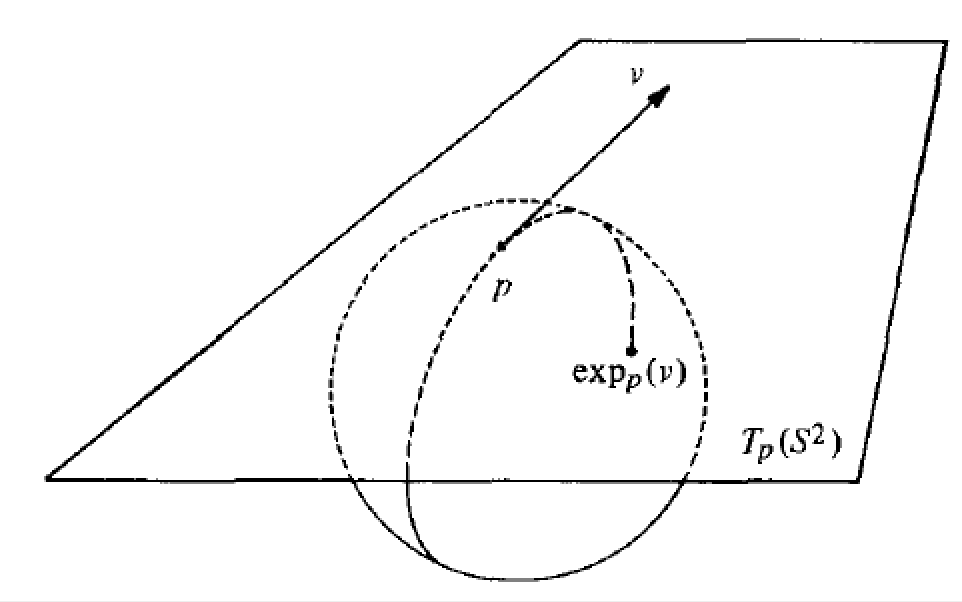
\includegraphics[scale = 0.4]{exp_map.png}}
\end{minipage}
\caption{\scriptsize
\textbf{The exponential map $\exp_{p}(\mb{v})$ is the point at $\cS$ obtained by laying off a length equal to $\norm{\mb{v}}{}$ along the geodesic that passes through $p$ in the direction of $\mb{v}$.  }}
\end{figure}
\begin{figure}[htb]
\centering
\begin{minipage}{0.6\linewidth}
 \centerline{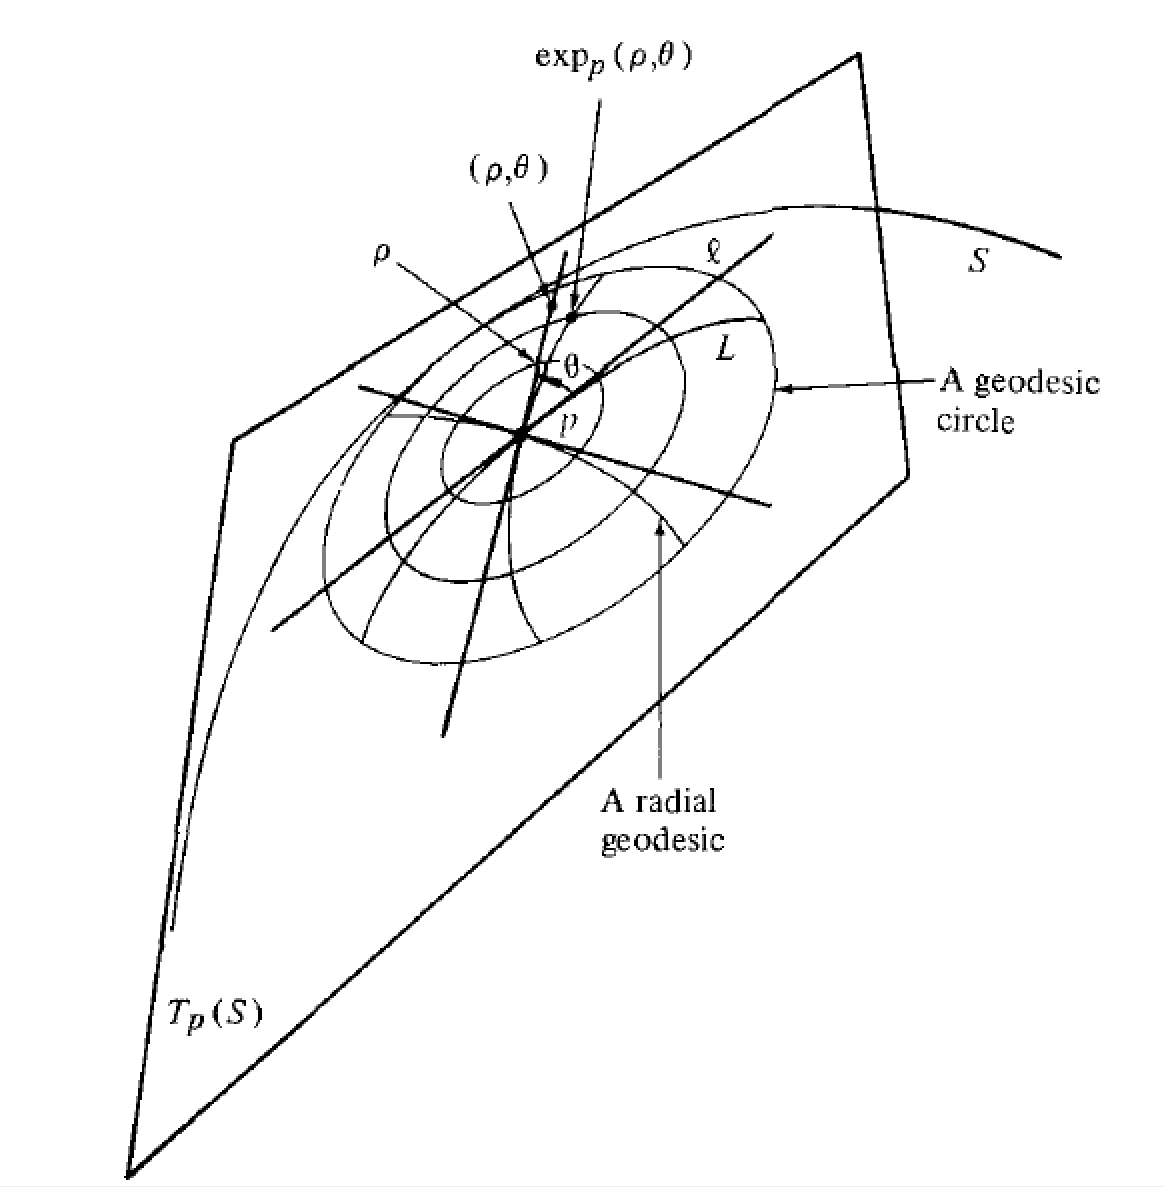
\includegraphics[scale = 0.4]{geo_polar_coord.png}}
\end{minipage}
\caption{\scriptsize
\textbf{The geodesic polar coordinate system is defined in the image of exponential map restricted to which the exponential map is a diffeomorphism.  Observe that the polar coordinate in the plane are not defined in the closed half line $\ell$ which corresponds to $\theta=0$. }}\vspace{-10pt}
\end{figure}

\item  \begin{definition}
By proposition , the exponential map $\exp_{p}: \mb{B}_{\epsilon}\subset T_{p}\cS \rightarrow \cS$ is a \emph{diffeomorphism} in a neighborhood $U \subset \mb{B}_{\epsilon}$ of the origin $0$ of $T_{p}\cS$. 

 The \emph{image} of the exponential map $V = \exp_{p}(U) \subset \cS$ of a neighborhood $U$ of the origin of $T_{p}\cS$ restricted to which $\exp_{p}$ is a diffeomorphism is called a \emph{normal neighborhood} of $p\in \cS$.\\
\end{definition}

\item \begin{definition} 
Given that $\exp_{p}$ is a diffeomorphism on $U$, it is possible to define a coordinate system on $V$. In particular, a polar coordinates can be defined in the tangent space $T_{p}\cS$ and referred as the \emph{geodesic polar coordinates}. 
  \end{definition}


\item In particular, choose in the tangent plane $T_{p}\cS, p\in \cS$, a system of polar coordinates $(\rho, \theta)$, where $\rho$ is the polar radius and $\theta, \; 0<\theta<2\pi$, is the polar angle, the pole of which is  the origin $0$ of $T_{p}\cS$. The point on $\cS$ is given by $\exp_{p}(\rho, \theta).$

Observe that the polar coordinate in the plane are not defined in the closed half line $\ell$ which corresponds to $\theta=0$. Set $\exp_{p}(\ell) = L$. Since $\exp_{p}: (U-\ell)\; \rightarrow (V-L)$ is still a diffeomorphism, we may parameterize the points of $(V-L)$ by the coordinates $(\rho, \theta)$, which are called \emph{geodesic polar coordinate system}. 

The image of $\exp_{p}: U\rightarrow V$ of circles in $U$, centered at $0$ is called \emph{geodesic circles} of $V$ and the image of $\exp_{p}$ of lines through $0$ will be called \emph{radical geodesics} of $V$ \citep{do1976differential}. In $V-L$, these are curves $\rho = const.$ and $\theta = const.$, respectively. 

\item \begin{remark} The Gaussian curvature $\mb{K}$ in a polar system $(\rho, \theta)$ satisfies 
\begin{align}
%\mb{K} &= -\frac{(\sqrt{G})_{\rho\rho}}{\sqrt{G}}\nonumber \\
%\text{or } 
\mb{K}\sqrt{G} &= -(\sqrt{G})_{\rho\rho} \nonumber %\label{eqn: Gauss_Jacobi_eqn}
\end{align}
called the \emph{Gauss-Jacobi equation}. \end{remark}



\item Consider the arc length $L(\rho)$ of the curve $\rho = const.$ between two close geodesics $\theta_{0}$ and $\theta_{1}$: 
\begin{align*}
L(\rho) &= \int_{\theta_{0}}^{\theta_{1}}\sqrt{G(\theta, \rho)}d\theta.
\end{align*}

Assume that $\mb{K}<0$ (hyperbolic geometry), since $\lim_{\rho\rightarrow 0}(\sqrt{G})_{\rho} = 1$, $\mb{K}\sqrt{G} = -(\sqrt{G})_{\rho\rho}$, the function $L(\rho)$ increases as $\rho$ increase, the geodesics $\theta_{0}$ and $\theta_{1}$ are getting farther and farther apart from each other. 

On the other hand, when $\mb{K}>0$ (elliptic geometry), the geodesics $\theta_{0}$ and $\theta_{1}$ may or may not come closer to each other after a certain value of $p$, and this depends on the Gaussian curvature. See Figure \ref{fig: arc_length_geo}.
\begin{figure}[tbh]
\centering
\begin{minipage}{0.6\linewidth}
 \centerline{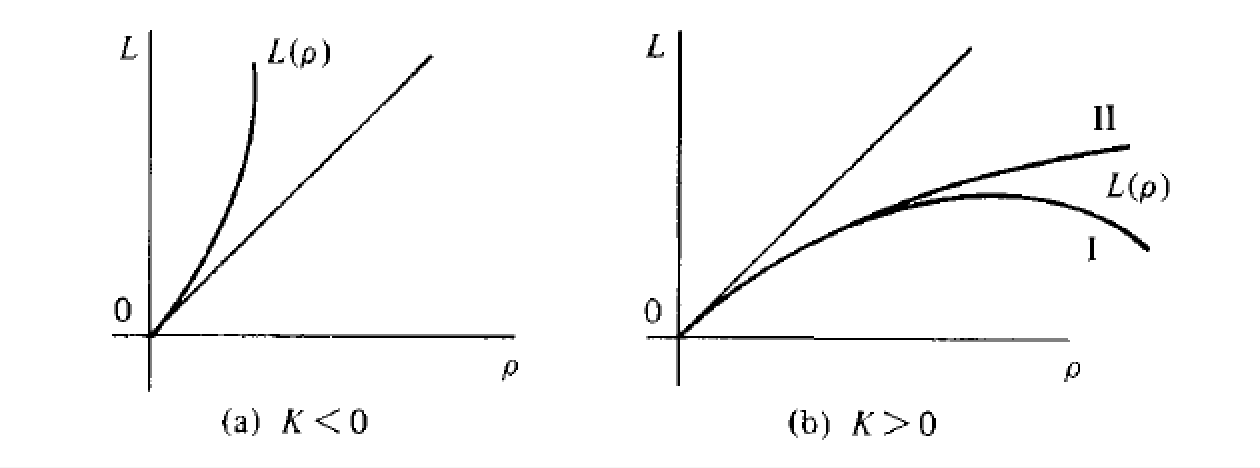
\includegraphics[scale = 0.43]{arc_length_geodesic.png}}
\end{minipage}\\
\begin{minipage}{0.6\linewidth}
 \centerline{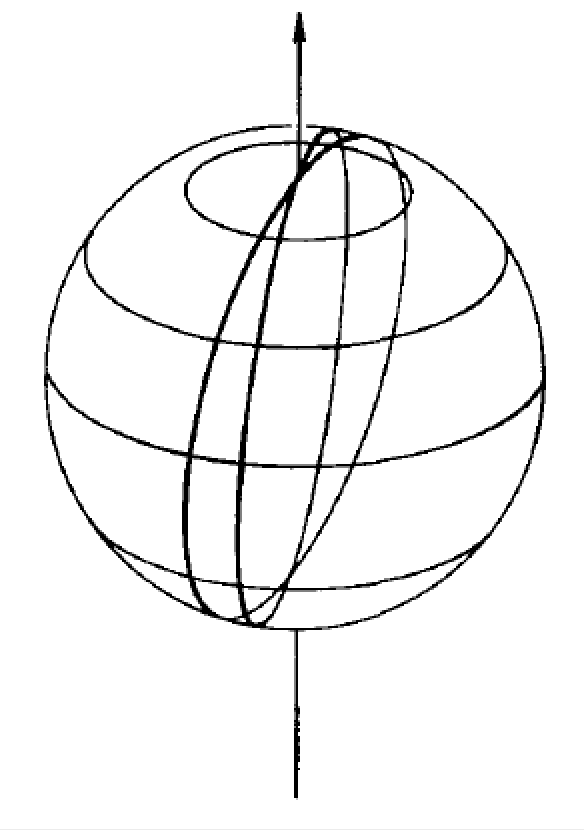
\includegraphics[scale = 0.43]{arc_length_geodesic2.png}}
\end{minipage}
\caption{\scriptsize
\textbf{The arc length of the geodesic joins two radical geodesics $\theta_{0}$ and $\theta_{1}$. For hyperbolic surface (a), the two radical geodesics will get farther apart as they depart from the origin. For the elliptic surface (b), these two geodesic may come closer after a certain point. Like in the sphere, two geodics become closer after passing the equator. }}\label{fig: arc_length_geo}\vspace{-10pt}
\end{figure}
\end{itemize}


\newpage
\section{Summary of shape operator $dN_{p}$}
\begin{enumerate}
\item The shape operator $dN_{p}: T_{p}S \rightarrow T_{p}S$ is a linear operator on the tangent space $T_{p}S$. It defines many intrinsic and extrinsic property of the surface. It is a self-adjoint operator. 

\item $dN_{p}(\mb{v})$ is the rate of change of the unit normal field $\mb{N}(p)$ along direction $\mb{v}$. As the normal field on the unit sphere, its rate of change will always be \emph{tangent to the surface}, thus $dN_{p}(\mb{v}) \in T_{p}S$.  

%\item In analogy as the curvature to the curve, $dN_{p}(\mb{v})$ on a neighborhood of $p\in \cS$ measures how rapidly the regular surface pull away from the tangent space $T_{p}S$ at $p$.

\item For a parameterized curve $\alpha(t)$ on $\cS$ with $\alpha(0) = p$, we restrict the normal vector $N$ to the curve $\alpha(t)$ and $N_{p}(\alpha'(0)) \equiv N'(0)$ measures the rate of change of normal vectors, restricted on the curve $\alpha(t)$ at $t=0$. It thus measures how $N$ pull away from $N(p)$ in the neighborhood of $p$.  In terms of this, $dN_{p} $ to $\cS(u,v)$  is in analogy of $k(s)$ for curve $\alpha(s)$.\\

\begin{figure}[thb]
\centering
\begin{minipage}{0.5\linewidth}
 \centerline{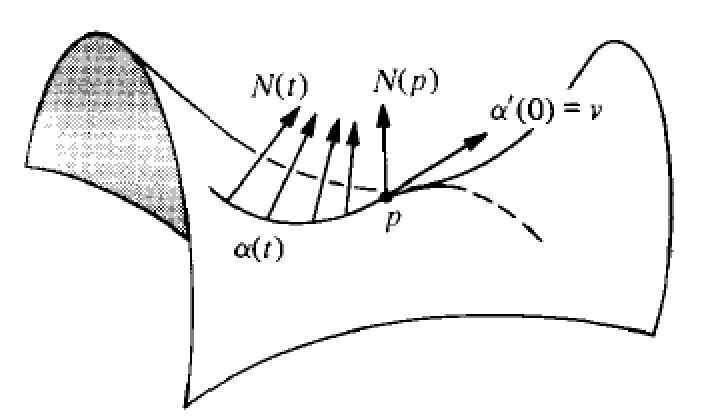
\includegraphics[scale = 0.55]{diff_gauss.png}}
\end{minipage}
\caption{\scriptsize
\textbf{The differential of Gauss map computed via restricting on the curve.}}
\end{figure}

\item   \begin{definition}
The determinant $\det{dN_{p}}$  is the \emph{Gaussian curvature} $\mb{K}$, which is an intrinsic curvature of the surface, i.e. it is invariant under isometries. 
\end{definition} 

\item The trace $-\text{tr}\paren{dN_{p}}$ is called the \emph{mean curvature} $\mb{H}$, which is an extrinsic curvature of the surface. 

\item The quadratic form of $\Pi_{p}(\mb{v}) = \inn{-dN_{p}(\mb{v})}{\mb{v}},$ for all $\mb{v}\in T_{p}S$ is the second fundamental form. It is the normal curvature of the surface along unit length direction $\mb{v}/\abs{\mb{v}}$ or the curvature of the normal section of the surface along direction $\mb{v}$. 

The second fundamental form is associated with the projection of the second-order derivatives of the parameterization along the normal direction of the surface. 

The second fundamental form is invariant under reparameterization and isometries. 
 
%\item For given $dN_{p}$, there exists an orthonormal basis $\set{\mb{e}_{1}, \mb{e}_{2}}$ in $T_{p}S$ such that $dN_{p}(\mb{e}_{1}) = -k_{1}\mb{e}_{1}$ and  $dN_{p}(\mb{e}_{2}) = -k_{2}\mb{e}_{2}$, $(k_{1}\ge k_{2})$ i.e. $\set{\mb{e}_{1}, \mb{e}_{2}}$ are eigenvectors of $-dN_{p}$ associated with eigenvalues $(k_{1}, k_{2})$. We also see that 
%$k_{1} = \max_{\norm{\mb{v}}{} = 1 }\Pi_{p}(\mb{v})$ and $k_{2} = \min_{\norm{\mb{v}}{} = 1 }\Pi_{p}(\mb{v})$.
%
%\begin{definition}  The \emph{maximum normal curvature} $k_{1}$ and the \emph{minimum normal curvature} $k_{2}$ are called the \emph{principal curvatures} at $p$; the corresponding directions, that is, the direction given by the eigenvectors $\mb{e}_{1}$ and $\mb{e}_{2}$, are called \emph{principal directions} at $p$.
%\end{definition} 
 
\item \begin{definition}  The eigenvalues and eigenvectors of $dN_{p}$ is called the \emph{principal curvature} and the \emph{principal directions}. It is given as the set of recursively maximum normal curvatures along a set of orthonormal directions.  We also see that $k_{\max} = \max_{\norm{\mb{v}}{} = 1 }\Pi_{p}(\mb{v})$ and $k_{\min} = \min_{\norm{\mb{v}}{} = 1 }\Pi_{p}(\mb{v})$.
\end{definition} 

\item  \begin{definition}
A point $p$ of a surface $\cS$ is called
\begin{itemize}
\item \emph{Elliptic}, if $\mb{K}= \det\paren{dN_{p}} >0$; \\
All curves passing through an \emph{elliptic} point $p$ have their normal vector pointing towards the same side of the tangent plane. The principal curvatures are of the same sign and the Gaussian curvature is positive. 

\item \emph{Hyperbolic}, if $\mb{K}=\det\paren{dN_{p}} <0$;\\
There are curves passing through an \emph{hyperbolic} point $p$ to have their normal vector pointing towards the any of the sides of the tangent plane. The principal curvatures are of the opposite sign and the Gaussian curvature is negative. 


\item \emph{Parabolic}, if  $\mb{K}=\det\paren{dN_{p}} =0$ but $dN_{p}\neq 0$;\\
At \emph{parabolic} point $p$, the Gaussian curvature is zero, but one of the principal curvature is nonzero. The points of a cylinder, e.g., are parabolic points. 

\item \emph{Planar}, if $dN_{p} = 0$.\\
At a \emph{planar} point, all principal curvatures are zero. The points in a plane satisfies this condition. An nontrival planer point, e.g. is the $(0,0,0)$ for the surface of revolution obtained by rotating the curve $z= y^{4}$ along the $z$-axis.   
\end{itemize}
\end{definition} 

\item  \begin{definition}
Let $p\in \cS$. An \emph{asymptotic direction} of $\cS$ at $p$ is a direction in $T_{p}S$ for which the normal curvature is zero, i.e. $\inn{dN_{p}(\mb{v}_{asym})}{\mb{v}_{asym}} = \Pi_{p}(\mb{v}_{asym})=0$. 
\end{definition} 

\item   \begin{definition}
At a point $p\in \cS$, two nonzero vectors $\mb{w}_{1}$ and $\mb{w}_{2}$ in $T_{p}S$ are \emph{conjugate}, if $\inn{dN_{p}(\mb{w}_{1})}{\mb{w}_{2}} = \inn{\mb{w}_{1}}{dN_{p(\mb{w}_{2})}} = 0$. Two directions $\mb{r}_{1}$ and $\mb{r}_{2}$ at $p$ are conjugate if a pair of nonzero vectors  $\mb{w}_{1}$ and $\mb{w}_{2}$ parallel to $\mb{r}_{1}$ and $\mb{r}_{2}$, respectively, are conjugate. 
\end{definition} 

\item For $p\in \cS$, the \emph{Dupin indicatrix} at $p$ is the set of vectors $\mb{w}$ of $T_{p}S$ such that $\Pi_{p}(\mb{w}) = \pm 1$. It can be viewed as the intersection of the surface with the plane parallel to $T_{p}S$ and close to $p$.
\end{enumerate}
\section{Summary of first and second fundamental form}
\begin{enumerate}
\item The \emph{first fundamental form} \citep{do1976differential} of a regular surface $\cS\subset \bR^{3}$ at $p\in \cS$ is defined as a  quadratic form,  $I_{p}: T_{p}S \rightarrow \bR$ given by 
\begin{align*}
I_{p}(\mb{w}) &= \inn{w}{w}_{p} = \norm{w}{2}^{2} \ge 0\; \; \mb{w}\in T_{p}S.
\end{align*}

\item  The quadratic form $\Pi_{p}$ defined in $T_{p}S$ by $\Pi_{p}(\mb{v}) = -\inn{dN_{p}(\mb{v})}{\mb{v}}$ is called the \emph{second fundamental form} of $\cS$ at $p$, where $dN_{p}$ is the differential of Gauss map at $p$, referred as the shape operator \citep{o2006elementary}. 

\item The coefficients for the first and second fundamental form
\begin{align}
E(u,v) &= \inn{\mb{x}_{u}}{\mb{x}_{u}} \nonumber\\
F(u,v) &= \inn{\mb{x}_{u}}{\mb{x}_{v}} \nonumber\\
G(u,v) &= \inn{\mb{x}_{v}}{\mb{x}_{v}} \nonumber \\
e(u,v)  &=  - \inn{N_{u}}{\mb{x}_{u}} = \inn{N}{\mb{x}_{uu}} \nonumber\\
f(u, v)&= - \inn{N_{u}}{\mb{x}_{v}} =  \inn{N}{\mb{x}_{vu}} =  \inn{N}{\mb{x}_{uv}} =  -\inn{N_{v}}{\mb{x}_{u}}\nonumber\\
g(u, v)&=   - \inn{N_{v}}{\mb{x}_{v}} = \inn{N}{\mb{x}_{vv}} \label{eqn: coeff_first_sec_fund_form}
\end{align}

\item See that $E,G$ are \emph{squared length of tangent vector along the coordinate curve} $\alpha(u, v_{0}), \text{with }\alpha_{u}' \equiv \mb{x}_{u}$ and $\alpha(u_{0}, v), \text{with }\alpha_{v}' \equiv \mb{x}_{v}$ .

Also, $e, g$ are seen as the \emph{normal curvature of the coordinate curve} $\alpha(u, v_{0}), \text{with }\alpha_{u}' \equiv \mb{x}_{u}$ and $\alpha(u_{0}, v), \text{with }\alpha_{v}' \equiv \mb{x}_{v}$, (i.e. the projection of second-order derivatives along $\mb{N}$) or curvature of the normal section of the surface along the direction $\mb{x}_{u}, \mb{x}_{v}$.

 The quantity $F$ measures the orthogonality between two coordinate curves (i.e. the angles). $F=0$ means that two coordinate curves are orthogonal to each other and $F=0 \Rightarrow f=0$. The quantity $f$ measures the projection of the rate of the change of vector field $\mb{x}_{u}$ w.r.t. the other coordinate curve $\alpha(u_{0}, v), \text{with }\alpha_{v}' \equiv \mb{x}_{v}$ along $\mb{N}$.


\item The coefficients of the second fundamental form $e,f,g$ are projection of the derivative of tangent plane along the normal direction of the plane, whereas the Christoffel symbols $\Gamma_{i,j}^{k}$ are the projections of the second-order derivatives of the coordinate curve, or the derivative of the tangent vector field along each basis of the tangent space. 

%\item 
\begin{itemize}
\item $E,F,G$ are quantities related to the \emph{first-order derivatives} of the coordinate curve (metric term in \emph{unit} velocity field);

\item The Christoffel symbols  $\Gamma_{i,j}^{k}$ determines  the projection of the second-order derivatives of the coordinate curve, or the derivative of the tangent vector field along each basis of the tangent space; that is, they determine the \emph{tangential component of the second-order derivatives} of the coordinate curve. It is a function of $E,F,G$ and its first derivatives. 

\item $e,f,g$ determines the \emph{normal component of the second-order derivatives} of the coordinate curve along $\mb{N}$;

\item The Gaussian curvature by Gaussian formula is related to the third-order derivatives of the coordinate curve (i.e. the differential of the Christoffel symbol). 
\end{itemize}

\item The Christoffel symbols $\Gamma_{i,j}^{k}$ only depends on the coefficients of the first fundamental form $E,F,G$ and its first-order derivatives. 

%Note that $E,G$ are \emph{squared length of tangent vector along the coordinate curve} $\alpha(u, v_{0}), \text{with }\alpha_{u}' \equiv \mb{x}_{u}$ and $\alpha(u_{0}, v), \text{with }\alpha_{v}' \equiv \mb{x}_{v}$ . Also $e, g$ are seen as the \emph{normal curvature of the coordinate curve} $\alpha(u, v_{0}), \text{with }\alpha_{u}' \equiv \mb{x}_{u}$ and $\alpha(u_{0}, v), \text{with }\alpha_{v}' \equiv \mb{x}_{v}$, (i.e. the projection of second-order derivatives along $\mb{N}$) or curvature of the normal section of the surface along the direction $\mb{x}_{u}, \mb{x}_{v}$.  Finally, $e,f,g$ are projection of the derivative of tangent plane along the normal direction of the plane, whereas the Christoffel symbols are the projections of this derivative along the tangent space. 
%
%The quantity $F$ measures the orthogonality between two coordinate curves (i.e. the angles). $F=0$ means that two coordinate curves are orthogonal to each other and $F=0 \Rightarrow f=0$. The quantity $f$ measures the projection of the rate of the change of vector field $\mb{x}_{u}$ w.r.t. the other coordinate curve $\alpha(u_{0}, v), \text{with }\alpha_{v}' \equiv \mb{x}_{v}$ along $\mb{N}$. 
%
%We can see that $E,F,G$ are quantities related to the first-order derivatives of the coordinate curve (metric term in \emph{unit} velocity field); $e,f,g$ and all Christoff symbols $\Gamma_{i,j}^{k}$ are related to the second-order derivatives of the coordinate curve, or the derivative of the tangent vector field: the Christoffel symbols determines its projection along the tangent space whereas $e,f,g$ determines its normal component along $\mb{N}$; the Gaussian curvature by Gaussian formula is related to the third-order derivatives of the coordinate curve (i.e. the differential of the Christoffel symbol). 
\end{enumerate}

\section{More understanding of parallel transport, covariant derivative and affine connection}
\begin{enumerate}
\item The notion of parallel transport or affine connection supplies a way of \emph{moving the local geometry} of a manifold \emph{along a curve}, or, \emph{connecting the tangent space of the nearby points}.

 Note that it is not well-defined to compare the tangent vector at one point with the tangent vector at another point. The parallel transport provides a way to define their relationship via affine transformation.

\item The notion of \emph{covariant derivative} and \emph{affine connection} are equivalent on the Riemannian manifold, whereas the covariant derivative is the \emph{infinitesimal parallel transport}. 

\item These concepts concern the rate of the change of a vector field $\mb{w}$ along a tangent direction $\mb{v} = \dot{\alpha}$ of a parameterized curve. Thus being denoted as $\nabla_{\mb{v}}\paren{\mb{w}}$. \\[5pt]

\item Intuition behind the affine connection:  note that the tangent plane is \emph{rolled} on $\cS$ without slipping or twisting, the point of contact traces out a curve on $\cS$. Conversely, given a curve on $\cS$, the tangent plane can be rolled along that curve. 

This provides a way to identify the tangent planes at different points along the curve: in particular, a tangent vector in the tangent space at \emph{one point} on the curve is identified with a unique tangent vector \emph{at any other point} on the curve. These identifications are always given by \emph{affine transformations} from \emph{one tangent plane to another}.

This notion of \emph{parallel transport} of tangent vectors, by affine transformations, along a curve has a \emph{characteristic} feature: the point of contact of the tangent plane with the surface always moves with the curve under \emph{parallel translation} (i.e., as the tangent plane is rolled along the surface, the \emph{point of contact} moves). When the point of contact is viewed as the \emph{origin} in the tangent plane (which is then a vector space), and the \emph{movement of the origin} is \emph{corrected by a translation}, so that parallel transport is \emph{linear}, rather than affine.
\begin{figure}[htb]
\centering
\begin{minipage}{0.6\linewidth}
 \centerline{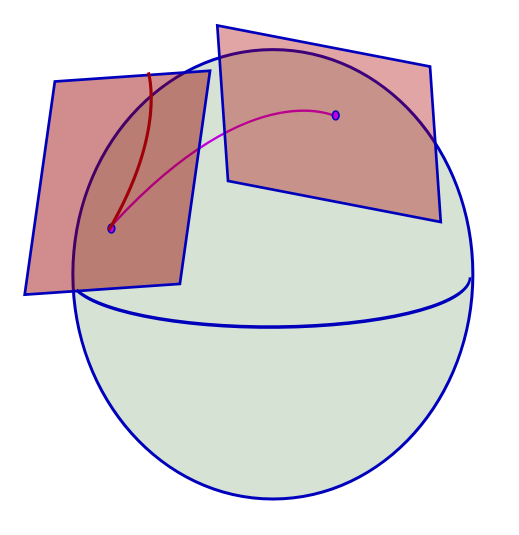
\includegraphics[scale = 0.32]{Parallel_transport_sphere.png}}
\end{minipage}
\caption{\scriptsize
\textbf{The geometric intuition behind the parallel transport along a curve: given a curve on the sphere, the tangent plane can be rolled on the curve without slipping or twisting.  Thus all the tangent plane on the curve can be identified via the affine transformation. }}\label{fig: parallel_transport_sphere}
\end{figure} \vspace{5pt}

\item Motivation of covariant derivative: In differentiating the vector field, the derivatives in component-wise manner do not transform in a manageable way under \emph{changes of coordinates}. In correcting this transformation, additional terms (i.e. the Christoffel symbols) are introduced so that the (corrected) derivative of one vector field along another transformed \emph{covariantly} under coordinate transformations. 

\item  \begin{remark}
Note that two surfaces are tangent along a curve $\alpha$ with a common vector $\mb{w}_{0} \in T_{\alpha(t)}S$ and $\mb{w} \in T_{\alpha(t)}\hat{S}$. Then the parallel transport $\mb{w}(t)$ of $\mb{w}_{0}$ relative to $\cS$ is the same as that relative to $\hat{\cS}$, as it has the same covariant derivative along the curve.

One can use this fact to find the parallel vector field along some curves. Assume that a regular curve $\alpha$ joins two points $p,q$ on $\cS$ and it is nowhere tangent to the asymptotic directions. Consider the envelop of the family of tangent planes of $\cS$ along $\alpha$. In a neighborhood of $\alpha$, this envelop is a regular surface $\Sigma$ which is tangent to $\cS$ along $\alpha$. Then we see that the parallel transport of $\mb{w}$ along $\alpha$ is the same no matter which surface $\cS$ or $\Sigma$ is concerned. 

 It can be shown that the Gaussian curvature of $\Sigma$ is zero, i.e. it is locally isometric to a plane. Hence, we can find a neighborhood $V\subset \Sigma$ of $p$ into a plane $P$ by an isometry $\varphi: V\rightarrow P$. To obtain the parallel transport of $\mb{w}$ along $V\cap \alpha$, we can take the usual parallel transport in the plane of $d\varphi_{p}(\mb{w})$ along $\varphi\circ  \alpha$. Then pull it back to $\Sigma$ by $d\varphi$.\\[10pt]
 \end{remark}

\item In surface in $\bR^{3}$, it is an \emph{affine connection}, satisfies the following properties: for $\mb{w}, \mb{v}, \mb{y}, \mb{z}$ the vector field in $U\subset \cS$ and $f: U \rightarrow \bR$ is a differentiable function in $\cS$; $\mb{y}\paren{f}$ is the directional derivative of $f$ in the direction of $\mb{y}$ (i.e. the direction derivative along the trajectory of vector field $\mb{y}$), $\lambda, \mu$ are real numbers, 
\begin{enumerate}
\item The affine property for vector field 
 \begin{align*}
\nabla_{\mb{y}}\paren{\lambda\mb{w}+ \mu\mb{v}} &= \lambda\nabla_{\mb{y}}\paren{\mb{w}}+ \mu\nabla_{\mb{y}}\paren{\mb{v}}; \\
\nabla_{\lambda\mb{y}+ \mu\mb{z}}\paren{\mb{w}} &= \lambda\nabla_{\mb{y}}\paren{\mb{w}}+ \mu\nabla_{\mb{z}}\paren{\mb{w}}
\end{align*}
\item The Leibniz rule
 \begin{align*}
\nabla_{\mb{y}}\paren{f\mb{w}} &= \mb{y}\paren{f}\mb{w}+ f\nabla_{\mb{y}}\paren{\mb{w}};\\
 \nabla_{f\mb{y}}\paren{\mb{v}} &=  f\nabla_{\mb{y}}\paren{\mb{v}};
\end{align*}
\item The metric-preserving property
\begin{align*}
\mb{y}\paren{\inn{\mb{w}}{\mb{v}}} &= \inn{\nabla_{\mb{y}}\paren{\mb{w}}}{\mb{v}} + \inn{\mb{w}}{\nabla_{\mb{y}}\paren{\mb{v}}};
\end{align*}
\item The symmetry property
\begin{align*}
\nabla_{\mb{e}_{i}}\paren{\mb{e}_{j}} &= \nabla_{\mb{e}_{j}}\paren{\mb{e}_{i}}, \quad \mb{e}_{i} = \mb{x}_{\xi_{i}}\text{ for parameterization }\mb{x}(\xi_{1},\ldots, \xi_{m}).
\end{align*}
\end{enumerate}
The first two properties defines the \emph{affine connection} in $U\subset \cS$. The last two properties associate the connection with the Riemannian metric and guarantee that the Christoffel symbols are symmetric w.r.t. lower indices.  These four properties defines the \emph{unique} connections or covariant derivatives, and parallel transport, geodesic on the surface. \\

\item The operator $\nabla: C^{\infty}(\cS, T\cS) \times C^{\infty}(\cS, T\cS)\rightarrow C^{\infty}(\cS, T\cS)$ 
\begin{align*}
(\mb{Y}, \mb{W})\mapsto \nabla_{\mb{Y}}\mb{W}
\end{align*} is referred as an \emph{affine connection} \citep{do1992riemannian, murray1993differential}, where $C^{\infty}(\cS, T\cS)$ is the space of differentiable vector fields on $\cS$, $T\cS = \set{(p,T_{p}\cS): p\in \cS}$ is the \emph{tangent bundle}.

Since $\nabla_{i}(f)$ on differentiable function $f$ is the partial derivatives $\partial_{i} f$, it is seen as a \emph{differential operator} on the \emph{tangent bundle} $T\cS$. The affine connection or the covariant derivative prescribe a way of differentiating vector fields. 

\item Note that the affine connection $\nabla_{\mb{y}}\mb{x}$ only depends on value of $\mb{y}$ at $p$ not the other points. \\[5pt]

\item In regular surface, the covariant derivative $\frac{D\mb{w}}{dt}$ is seen as tangential projection of the Euclidean derivative of the field $\mb{w}$ along a curve. 
\begin{align*}
\frac{D\mb{w}}{dt} &= \mathcal{P}_{T_{p}S}\paren{\frac{d\mb{w}}{dt} }.
\end{align*}

\item In coordinate neighborhood, we can describe the covariant derivative of a vector field $\mb{w}$ along another vector field $\mb{v}$ at $p$ as, in each coordinate, the partial derivatives of the component function with additional linear transformation of coordinate axis; that is, for $\mb{w} = \sum_{k}w_{k}\mb{e}_{k}$ and $\mb{v} = \sum_{k}v_{k}\mb{e}_{k}$ in $T_{p}\cS$, then 
\begin{align*}
\nabla_{\mb{v}}\mb{w} &=\sum_{k} \paren{ \sum_{i}v_{i}\paren{\partial_{i}w_{k}} + \sum_{i,j}v_{i}\Gamma_{i,j}^{k}w_{j} }\mb{e}_{k}
\end{align*}
or in each component 
\begin{align*}
(\nabla_{\mb{v}}\mb{w})^{k} &= \paren{v_{i}\paren{\partial_{i}w_{k}} + v_{i}\Gamma_{i,j}^{k}w_{j} }\mb{e}_{k},
\end{align*}
where we ignore the summation over common indices $i,j$.

Also \begin{align*}
\nabla_{i}\mb{e}_{j}&= \mb{e}_{k}\Gamma_{i,j}^{k}
\end{align*}


\item The \emph{unit length vector field} $\mb{v}$ that is \emph{parallel} along a curve $\alpha$, i.e.  $\frac{D\mb{v}}{dt} = 0$ for every $t\in I$ is used as a \emph{reference} when considering the connection of the geometries of the unit length vector field $\mb{w}$ at different point along $\alpha$. 

That is, define a differentiable map $\varphi: I \rightarrow \bR$ to be the angle from $\mb{v}(t)$ to $\mb{w}(t)$ in the orientation of the surface. Then the parallel transport of $\mb{w}$ at $p=\alpha(t)$ along direction $\dot{\alpha}(t)$ is given by 
\begin{align*}
\nabla_{\dot{\alpha}(t)}\mb{w} &= \frac{d\varphi}{dt}\,\paren{\mb{N}\wedge \mb{w}},
\end{align*}
where $d\varphi/dt = k_{g} = \inn{d\mb{w}/dt}{\mb{N}\wedge \mb{w}}$ is the geodesic curvature. 

Two unit vector fields that are \emph{both parallel} along a curve if and only if the angle btw them is fixed as moving along the curve.\\



 
\item The (unit) velocity field $\dot{\gamma}(t)$ of a \emph{geodesic} $\gamma(t)$ is parallel along $\gamma(t)$, i.e. $\frac{D\dot{\gamma}}{dt} = \nabla_{\dot{\gamma}}\dot{\gamma} = 0$, which makes it a natural \emph{referential vector field} on the surface.\\[5pt]

\item On any manifold of positive dimension there are infinitely many affine connections. When the Riemannian metric is defined, then there is a unique natural choice of connection (via the inverse and derivatives of the Riemannian metric), called \emph{Levi-Civita connection}.
\end{enumerate}
\newpage
\section{Theorems and Properties for curves and surfaces}
\subsection{curves and surfaces}
\begin{itemize}
\item 
\begin{theorem}\label{th: curv_tri}
\emph{(the fundamental theorem of the local theory of curves)}\\
Given differentiable functions $k(s)>0$ and $\tau(s)$ for $s\in I$, there exists a regular parameterized curve $\alpha: I\rightarrow \bR^{3}$ such that $s$ is the arc length, $k(s)$ is the curvature and $\tau(s)$ is the torsion. Moreover, any other curve $\hat{\alpha}$ satisfying the conditions above differ from $\alpha$ by a rigid transformation as $\hat{\alpha} = \rho\circ \alpha + c$ for $\rho$ a orthogonal transformation and $c$ a translation vector. 
\end{theorem}\vspace{5pt}

\item \begin{theorem}\label{th: surf_difffun}
If $f: U\subset \bR^{2} \rightarrow \bR$ is a differentiable function in an open set $U$ of $\bR^{2}$, then the graph of $f$, $(u,v, f(u,v))$ is a regular surface in $\bR^{3}$ for $(u,v) \in U$.
\end{theorem}

\item  \begin{theorem}\label{th: surf_regval}
If $F: U \subset \bR^{3} \rightarrow \bR$ is a differentiable function in an open set $U$ of $\bR^{3}$, and $r\in F(U)$ is a regular value of $F$,  then the pre-image of $F$ at $r$, $F^{-1}(r)$ is a regular surface in $\bR^{3}$.
\end{theorem}\vspace{5pt}

\item \begin{proposition}\label{prop: tang_param}
Let $\mb{x}: U\subset \bR^{2} \rightarrow \cS$ be a parameterization of a regular surface $\cS$ and let $q\in U$. The tangent plane to $\cS$ at $\mb{x}(q)$ is given as 
\begin{align*}
d\mb{x}_{q}\paren{\bR^{2}} \subset \bR^{3}
\end{align*} as a $2-$dimensional linear subspace.
\end{proposition}


\item \begin{proposition}\label{prop: local_diff_fun}
Let $\cS\subset \bR^{3}$ be a regular surface and $p\in \cS$. Then there exists a neighborhood $V$ of $p$ in $\cS$ such that $V$ is the graph of a differentiable function which has one of the following three forms: 
\begin{align*}
z = f(x,y),\quad y= g(x,z), \quad x= h(y,z). 
\end{align*}
\end{proposition}


\item \begin{theorem}\label{th: inver_fun}
If $\cS_{1}$ and $\cS_{2}$ are two regular surfaces and $\varphi: U\subset \cS_{1} \rightarrow \cS_{2}$ is a differentiable mapping of an open subset $U\subset \cS_{1}$ such that the differential $d\varphi_{p}$ of $\varphi$ at $p$ is an isomorphism, then $\varphi$ is a local diffeomorphism at $p$.
\end{theorem}\vspace{10pt}
\end{itemize}

\subsection{Gauss map}
\begin{itemize}
\item \begin{proposition}\label{prop: Gauss_selfadj}
The differential $dN_{p}:  T_{p}S \rightarrow T_{p}S$ of the Gauss map is a self-adjoint linear map, i.e. $\inn{dN_{p}(\mb{w}_{1})}{\mb{w}_{2}} = \inn{\mb{w}_{1}}{dN_{p}(\mb{w}_{2})}  $ for $\set{\mb{w}_{1}, \mb{w}_{2}}$ any two vectors in $T_{p}S$. 
\end{proposition}
\begin{proof}
It suffice to show that $\inn{dN_{p}(\mb{w}_{1})}{\mb{w}_{2}} = \inn{\mb{w}_{1}}{dN_{p}(\mb{w}_{2})}  $ for $\set{\mb{w}_{1}, \mb{w}_{2}}$ the basis in $T_{p}S$. Let $\mb{x}(u,v)$ be a parameterization of the surface $\cS$ at $p$ and the $\set{\mb{x}_{u}, \mb{x}_{v}}$ be the basis for $T_{p}S$. If $\alpha(t) = \mb{x}(u(t), v(t))$ is a parameterized curve in $\cS$ with $\alpha(0) = p$, we have 
\begin{align*}
dN_{p}(\alpha'(0)) &= dN_{p}( \mb{x}_{u}u'(0) + \mb{x}_{v}v'(0) )\\
&= \rlat{\frac{d}{dt}N(u(t), v(t) )}{t=0}\\
&= dN_{u}u'(0) + dN_{v}v'(0)
\end{align*} with $dN_{u} = dN_{p}( \mb{x}_{u})$ and  $dN_{v} = dN_{p}( \mb{x}_{v})$.

To show the self-adjoint property, it suffice to show that $\inn{dN_{u}}{\mb{x}_{v}} = \inn{\mb{x}_{u}}{dN_{v}}$. To show this, we take derivative of $\inn{N}{\mb{x}_{u}} = 0$ and $\inn{N}{\mb{x}_{v}} = 0$ with respect to $v$ and $u$, respectively, and obtain
\begin{align*}
\inn{dN_{v}}{\mb{x}_{u}}  + \inn{N}{\mb{x}_{u,v}} = 0\\
\inn{dN_{u}}{\mb{x}_{v}}  + \inn{N}{\mb{x}_{v,u}} = 0
\end{align*}
Thus
\begin{align*}
\inn{dN_{v}}{\mb{x}_{u}}  = -  \inn{N}{\mb{x}_{u,v}}  = \inn{dN_{u}}{\mb{x}_{v}}.   \qed
\end{align*}
\end{proof}

\item \begin{theorem}(Meusnier) \label{th: meusnier}\\
All curves lying on a surface $\cS$ and having at a given point $p\in \cS$ the same tangent line have at this point the same normal curvatures. 
\end{theorem}
\begin{figure}[thb]
\centering
\begin{minipage}{0.6\linewidth}
 \centerline{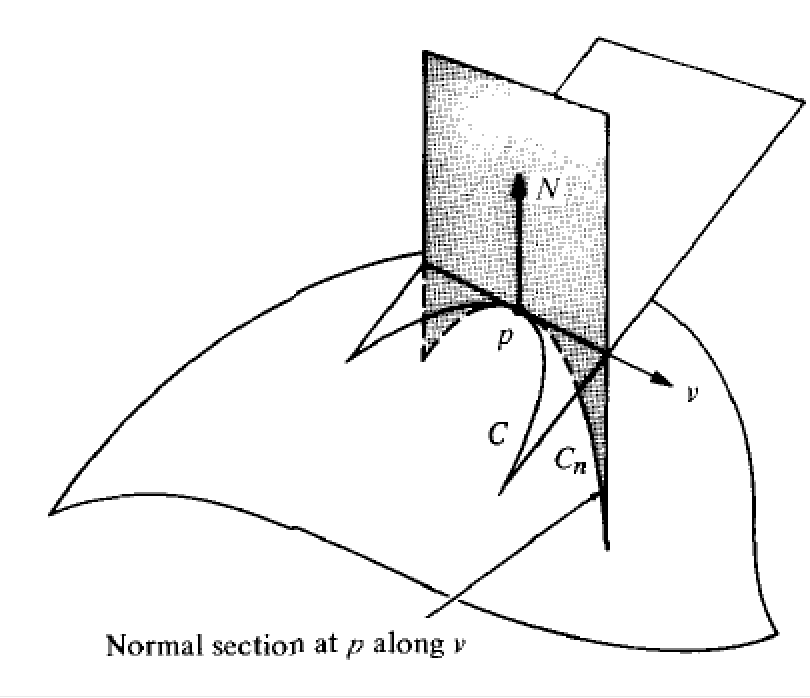
\includegraphics[scale = 0.43]{meusnier.png}}
\end{minipage}
\caption{\scriptsize
\textbf{The curve $\cC$ and $\cC_{n}$ have the same normal curvature. The dashed line $\cC_{n}$ is the normal section of $\cS$ at $p$ along the direction $\mb{v}$, which is the intersection between $\cS$ and the plane spanned by $N(p)$ and $\mb{v}$. By Meusnier's proposition, (the absolute value of) the normal curvature of the curve $\cC$ at $p$ (solid line) is equal to the  curvature of the normal section $\cC_{n}$ (dashed line) of $\cS$ at $p$ along $\alpha'(0)$. }}
\end{figure}
\begin{proof}
For the second fundamental form $\Pi_{p}$, consider a regular curve $\cC \subset \cS$ parameterized by $\alpha(s)$, where $s$ is the arc length, and $\alpha(0) = p$. If we denote by $N(s)$ the restriction of the normal vector $N$ to the curve $\alpha(s)$, we have $\inn{N(s)}{\alpha'(s)} = 0$. Hence 
\begin{align*}
\inn{N(s)}{\alpha''(s)} = - \inn{N'(s)}{\alpha'(s)}.
\end{align*}
Therefore
\begin{align*}
\Pi_{p}(\alpha'(0)) &= -\inn{dN_{p}(\alpha'(0))}{\alpha'(0)}\\
&= -\inn{N'(0)}{\alpha'(0)} = \inn{N(0)}{\alpha''(0)}\\
&= k\inn{N}{\mb{n}}(p) = k_{n}(p). 
\end{align*}

In other words, the value of $\Pi_{p}(\mb{v})$ for unit vector $\mb{v}\in T_{p}S$ is equal to the normal curvature of a regular curve passing through $p$ and tangent to $\mb{v}$. If $\mb{v}_{1} = \mb{v}_{2}$ for two curves $\cC_{1}$ and $\cC_{2}$, then $\Pi_{p}(\mb{v}_{1}) = k_{n1} = k_{n2} = \Pi_{p}(\mb{v}_{2})$. \qed
\end{proof}\vspace{15pt}
\end{itemize}

\subsection{Intrinsic geometry of surfaces}
\begin{itemize}
\item \begin{proposition}\label{prop: local_iso}
Assume the existence of parameterization $\mb{x}: U\rightarrow \cS$ and $\bar{\mb{x}}: U\rightarrow \bar{\cS}$ such that $E=\bar{E}$, $F=\bar{F}$, $G=\bar{G}$ in $U$. Then the map $\varphi= \bar{\mb{x}}\circ \mb{x}^{-1}:  \mb{x}(U) \rightarrow \bar{\cS}$ is a local isometry. 
\end{proposition}
\begin{proof}
Let $p\in \mb{x}(U)$, and $\mb{w}\in T_{p}S$. Then  $\mb{w}$ is tangent to a curve $\mb{x}(\beta(t))$ at $t=0$, where $\beta(t) = (u(t), v(t))$ is a curve in $U$; thus, $\mb{w}$ can be written as (at $t=0$)
\begin{align*}
\mb{w} &= \mb{x}_{u}u' + \mb{x}_{v}v'
\end{align*} for $\set{\mb{x}_{u}, \mb{x}_{v}}$ basis in $T_{p}S$.

By definition, the vector $d\varphi_{p}(\mb{w})$ is the tangent vector to the curve $\varphi\circ \mb{x}\circ\beta(t) = \bar{\mb{x}}\circ\beta(t) = \bar{\mb{x}}(\beta(t))$, i.e. 
\begin{align*}
d\varphi_{p}(\mb{w}) &= \bar{\mb{x}}_{u}u' + \bar{\mb{x}}_{v}v'
\end{align*}

Since 
\begin{align*}
I_{p}(\mb{w}) &= E(u')^{2} + 2F(u'v')+ G(v')^{2}\\
I_{\varphi(p)}(d\varphi_{p}(\mb{w}))&= \bar{E}(u')^{2} + 2\bar{F}(u'v')+ \bar{G}(v')^{2}, 
\end{align*}
we conclude that $I_{p}(\mb{w})  = I_{\varphi(p)}(d\varphi_{p}(\mb{w}))$ for all $p\in \mb{x}(U)$ and for all $\mb{w}\in T_{p}S$; hence, $\varphi$ is an isometry. \qed
\end{proof}\vspace{15pt}


\item \begin{theorem} \label{th: Gauss_theorem}
(THEOREMA EGREGIUM by Gauss)\\
The Gaussian curvature $\mb{K}$ of a surface is invariant by local isometries. 
\end{theorem}
\begin{proof}
Given parameterization $\mb{x}: U \rightarrow \cS$ and a point $p\in \cS$, the trihedron $(\mb{x}_{u}, \mb{x}_{v}, N)$ at $p$ form a basis in ambient space. We consider the expression, 
\begin{align}
\paren{\mb{x}_{uu}}_{v} - \paren{\mb{x}_{uv}}_{u} &= 0.  \label{eqn: Gauss_theorem_1}
\end{align}
By fact that $\mb{x}_{uu}, \mb{x}_{uv}$ lies in the space spanned by $(\mb{x}_{u}, \mb{x}_{v}, N)$ at $p$, using the Christoffel symbol, we have the following equations
\begin{align}
\mb{x}_{uu} &= \Gamma_{11}^{1}\mb{x}_{u} + \Gamma_{11}^{2}\mb{x}_{v} + e\mb{N}\nonumber\\
\mb{x}_{uv} &= \Gamma_{12}^{1}\mb{x}_{u} + \Gamma_{12}^{2}\mb{x}_{v} + f\mb{N}\nonumber\\
\mb{x}_{vv} &= \Gamma_{22}^{1}\mb{x}_{u} + \Gamma_{22}^{2}\mb{x}_{v} + g\mb{N}\nonumber\\
\mb{N}_{u} &= a_{11}\mb{x}_{u} + a_{21}\mb{x}_{v}
\nonumber\\
\mb{N}_{v} &= a_{12}\mb{x}_{u} + a_{22}\mb{x}_{v} \label{eqn: Gauss_theorem_2}
\end{align} 
and substitute the above equations into \eqref{eqn: Gauss_theorem_1}, we obtain
\begin{align*}
\Gamma_{11}^{1}\mb{x}_{uv} + \Gamma_{11}^{2}\mb{x}_{vv} + e\mb{N}_{v}
&+\paren{\Gamma_{11}^{1}}_{v}\mb{x}_{u} + \paren{\Gamma_{11}^{2}}_{v}\mb{x}_{v}+ e_{v}\mb{N}\\
&= \Gamma_{12}^{1}\mb{x}_{uu} + \Gamma_{12}^{2}\mb{x}_{uv} + f\mb{N}_{u}\\
&+ \paren{\Gamma_{12}^{1}}_{u}\mb{x}_{u} + \paren{\Gamma_{12}^{2}}_{u}\mb{x}_{v} + f_{u}\mb{N} \\[5pt]
\Leftrightarrow \paren{\Gamma_{11}^{1}\mb{x}_{uv} + \Gamma_{11}^{2}\mb{x}_{vv} - \Gamma_{12}^{1}\mb{x}_{uu} - \Gamma_{12}^{2}\mb{x}_{uv} }
&= \paren{\paren{\Gamma_{12}^{1}}_{u}-\paren{\Gamma_{11}^{1}}_{v}}\mb{x}_{u} + \paren{  \paren{\Gamma_{12}^{2}}_{u}- \paren{\Gamma_{11}^{2}}_{v}}\mb{x}_{v}\\
& +\paren{f\mb{N}_{u} - e\mb{N}_{v}}+ \paren{f_{u}-e_{v}}\mb{N}
\end{align*}
Substitute \eqref{eqn: Christoffel_eq_2} into above equations, and the LHS is 
\begin{align*}
&\Gamma_{11}^{1}\paren{\Gamma_{12}^{1}\mb{x}_{u} + \Gamma_{12}^{2}\mb{x}_{v} + f\mb{N}} + \Gamma_{11}^{2}\paren{\Gamma_{22}^{1}\mb{x}_{u} + \Gamma_{22}^{2}\mb{x}_{v} + g\mb{N}}\\
& - \Gamma_{12}^{1}\paren{\Gamma_{11}^{1}\mb{x}_{u} + \Gamma_{11}^{2}\mb{x}_{v} + e\mb{N}} - \Gamma_{12}^{2}\paren{\Gamma_{12}^{1}\mb{x}_{u} + \Gamma_{12}^{2}\mb{x}_{v} + f\mb{N}}\\
&=   \paren{\Gamma_{11}^{1}\Gamma_{12}^{1} +   \Gamma_{11}^{2}\Gamma_{22}^{1} - \Gamma_{12}^{1}\Gamma_{11}^{1}   - \Gamma_{12}^{2}\Gamma_{12}^{1}  }\mb{x}_{u} 
+  \paren{\Gamma_{11}^{1}\Gamma_{12}^{2} + \Gamma_{11}^{2}\Gamma_{22}^{2} - \Gamma_{12}^{1}\Gamma_{11}^{2}     - \paren{\Gamma_{12}^{2}}^{2}  }\mb{x}_{v} \\
& + \paren{\Gamma_{11}^{1}f + \Gamma_{11}^{2}g   - \Gamma_{12}^{1}e - \Gamma_{12}^{2}f }\mb{N}
\end{align*}
And the RHS
\begin{align*}
&\paren{\paren{\Gamma_{12}^{1}}_{u}-\paren{\Gamma_{11}^{1}}_{v}}\mb{x}_{u} +\paren{  \paren{\Gamma_{12}^{2}}_{u}- \paren{\Gamma_{11}^{2}}_{v}}\mb{x}_{v} +\paren{f\mb{N}_{u} - e\mb{N}_{v}}+ \paren{f_{u}-e_{v}}\mb{N}\\
&=\paren{\paren{\Gamma_{12}^{1}}_{u}-\paren{\Gamma_{11}^{1}}_{v} + a_{11}f - a_{12}e}\mb{x}_{u}
+\paren{\paren{\Gamma_{12}^{2}}_{u}- \paren{\Gamma_{11}^{2}}_{v} + a_{21}f - a_{22}e}\mb{x}_{v}+ \paren{f_{u}-e_{v}}\mb{N} 
\end{align*}

Thus we have the equation as 
\begin{align*}
A_{1}\mb{x}_{u}+ B_{1}\mb{x}_{v}+ C_{1}\mb{N} &= 0
\end{align*}
where
\begin{align}
A_{1} &= -\paren{\Gamma_{12}^{1}}_{u}+\paren{\Gamma_{11}^{1}}_{v} +   \Gamma_{11}^{2}\Gamma_{22}^{1}  - \Gamma_{12}^{2}\Gamma_{12}^{1}- a_{11}f+ a_{12}e\nonumber\\
B_{1} &= -\paren{\Gamma_{12}^{2}}_{u}+ \paren{\Gamma_{11}^{2}}_{v} - a_{21}f + a_{22}e+ \Gamma_{11}^{1}\Gamma_{12}^{2} + \Gamma_{11}^{2}\Gamma_{22}^{2} - \Gamma_{12}^{1}\Gamma_{11}^{2} - \paren{\Gamma_{12}^{2}}^{2}\nonumber\\
C_{1} &=  -f_{u}+e_{v}+ \Gamma_{11}^{1}f + \Gamma_{11}^{2}g   - \Gamma_{12}^{1}e - \Gamma_{12}^{2}f \nonumber
\end{align}
By independence of $(\mb{x}_{u}, \mb{x}_{v}, N)$ at $p$, $A_{1}=0, B_{1}=0, C_{1} = 0$, and by \eqref{eqn: weingarten}, we have for $B_{1} = 0$
\begin{align}
\paren{\Gamma_{12}^{2}}_{u}- \paren{\Gamma_{11}^{2}}_{v} - \Gamma_{11}^{1}\Gamma_{12}^{2} - \Gamma_{11}^{2}\Gamma_{22}^{2} + \Gamma_{12}^{1}\Gamma_{11}^{2} +\paren{\Gamma_{12}^{2}}^{2} &=- a_{21}f + a_{22}e\nonumber\\
%&= - \frac{eF- fE}{EG- F^{2}}f +  e\frac{fF- gE}{EG- F^{2}}\\
%&= \frac{1}{EG- F^{2}}\paren{-efF +f^{2}E + efF - egE  }\nonumber\\
&= -\frac{eg - f^{2}}{EG- F^{2}}E \nonumber\\
&= -\mb{K}E \label{eqn: Gauss_theorem_3}
\end{align}
Similarly for $A_{1} = 0$
\begin{align*}
\paren{\Gamma_{12}^{1}}_{u}-\paren{\Gamma_{11}^{1}}_{v} -   \Gamma_{11}^{2}\Gamma_{22}^{1}  + \Gamma_{12}^{2}\Gamma_{12}^{1}&= - a_{11}f+ a_{12}e\\
&= F\frac{eg - f^{2}}{EG- F^{2}}\\
&=\mb{K}F 
\end{align*}

Note that by \eqref{eqn: Gauss_theorem_3}, the Gaussian curvature $\mb{K}$ only on the coefficient of first fundamental form $E$, and the Christoffel symbols $\Gamma_{11}^{1}, \Gamma_{11}^{2},  \Gamma_{12}^{1}, \Gamma_{12}^{2}, \Gamma_{22}^{2} $ and their derivatives $\paren{\Gamma_{12}^{2}}_{u}, \paren{\Gamma_{11}^{2}}_{v}$ , which is invariant under local isometries. \qed
\end{proof}\vspace{10pt}

\item 
\begin{theorem} \label{th: Bonnet_th}
(Bonnet). Let $E,F,G, e,f,g$ be differentiable functions defines in an open set $V\subset \bR^{2}$, with $E>0, G>0$. Assume that the given functions satisfies formally the Gauss and Mainardi-Codazzi equations and that $EG-F^{2} >0$. Then, for every $q\in V$, there exits a neighborhood $U\subset V$  of $q$ and a diffeomorphism $\mb{x}: U \rightarrow \mb{x}(U)\subset \bR^{3}$ such that the regular surface $ \mb{x}(U)\subset \bR^{3}$ has $E,F,G,e,f,g$ as a coefficient of the first and second fundamental forms, respectively. Furthermore, if $U$ is connected and if $\hat{\mb{x}}: U \rightarrow \hat{\mb{x}}(U)\subset \bR^{3}$ is another diffeomorphism satisfying the same conditions, then there exits a proper linear orthogonal transformation $\rho$ and translation $T$ so that $\hat{\mb{x}} = T \circ \rho \circ \mb{x}$. 
\end{theorem}
\end{itemize}

\subsection{Parallel transport and geodesic}
\begin{itemize}
\item 
\begin{proposition}\label{prop: para_transp}
Let $\mb{w}, \mb{v}$ be parallel vector fields along $\alpha: I\rightarrow \cS$. Then $\inn{\mb{w}(t)}{\mb{v}(t)}$ is constant.  In particular, $\abs{\mb{w}(t)}$ and $\abs{\mb{v}(t)}$ are constant, and the angle between $\mb{w}, \text{and }\mb{v}$ is constant. 
\end{proposition}
\begin{proof}
Note that $\mb{w}$ is parallel along $\alpha$, which means that $\frac{D\mb{w}}{dt} =0$, or the differential of the vector field $\frac{d\mb{w}}{dt}$ is orthogonal to the tangent space $T_{\alpha(t)}\cS$, i.e.
\begin{align*}
\inn{\mb{w}'}{\mb{v}} &= 0;\quad \forall t\in I.
\end{align*}
Similarly, $\inn{\mb{w}}{\mb{v}'} = 0; \;\forall t\in I$. Therefore
\begin{align*}
\paren{\inn{\mb{w}(t)}{\mb{v}(t)}}' &= \inn{\mb{w}}{\mb{v}'}+ \inn{\mb{w}'}{\mb{v}} = 0,\;
\end{align*}
i.e. $\inn{\mb{w}(t)}{\mb{v}(t)} = c,\;\;\forall t\in I. $ \qed
\end{proof}\vspace{10pt}

\item \begin{proposition}\label{prop: para_transp_curv}
Let $\alpha: I\rightarrow \cS$ be a parameterized curve in $\cS$ and let $\mb{w}_{0} \in T_{\alpha(t_{0})}S,\; t_{0}\in I$. There exists a unique parallel vector field $\mb{w}(t)$ along $\alpha(t)$, with $\mb{w}(t_{0}) = \mb{w}_{0}$. 
\end{proposition}
It shows that there exists a unique vector field that is parallel along any given regular curve and it only depends on one initial vector in the tangent space. \\

\item \begin{proposition}\label{prop: geo_unique}
Given a point $p\in \cS$ and a vector $\mb{w}\in T_{p}(\cS), \mb{w}\neq 0$, there exists an $\epsilon>0$ and a unique parameterized geodesic $\gamma: (-\epsilon, \epsilon) \rightarrow \cS$ such that $\gamma(0)=p$ and $\gamma'(0) = \mb{w}$.
\end{proposition}\vspace{15pt}


\item \begin{lemma}\label{lem: diff_angle}
Let $a,b$ be differentiable functions in $I$ with $a^{2}+ b^{2} = 1$ and $\phi_{0}$ be such that $a_{0} = \cos \phi_{0}$ and $b_{0} = \sin \phi_{0}$. Then the differentiable function 
\begin{align*}
\phi &= \phi_{0} + \int_{t_{0}}^{t}\paren{ab' - a'b}dt
\end{align*}
is such that $\cos \phi = a(t)$ and $\sin \phi = b(t), t\in I,$ and $\phi\paren{t_{0}} = \phi_{0}$.
\end{lemma}

\begin{lemma} \label{lem: cov_deriv_angle}
Let $\mb{v,w}$ be two differentiable vector fields along the curve $\alpha: I \rightarrow \cS$, with $\abs{\mb{w}(t)} = \abs{\mb{v}(t)} = 1$, $t\in I$. Then 
\begin{align*}
\brac{\frac{D\mb{w}}{dt}} - \brac{\frac{D\mb{v}}{dt}} &= \frac{d\phi}{dt},
\end{align*}
where $\phi$ is one of the differentiable determination of the angle from $\mb{v}$ to $\mb{w}$, as given in Lemma \ref{lem: diff_angle}
\end{lemma}
\end{itemize}
\subsection{The Gauss-Bonnet theorem with non-Euclidean geometry}
\begin{itemize}
\item We states the local version of the Gauss-Bonnet Theorem
\begin{theorem}\label{thm: gauss_bonnet_local}  (\textbf{Gauss-Bonnet Theorem (Local)}) \citep{do1976differential}\\
Let $\mb{x}: U \rightarrow \cS$ be an \textbf{isothermal parametrization} (i.e., $F = 0, E = G = \lambda^2(u, v)$) of an oriented surface $\cS$, where $U \subset \cR^2$ is \textbf{homeomorphic} to an \textbf{open disk} and $\mb{x}$ is compatible with the orientation of $\cS$. Let $\cR \subset \mb{x}(U)$ be a \textbf{simple region} of $\cS$ and let $\alpha: I \rightarrow \cS$ be such that  $\partial \cR = \alpha(I)$. Assume that $\alpha$ is \textbf{positively oriented}, parametrized by arc length $s$, and let $\alpha(s_0),\ldots, \alpha(s_k)$ and $\theta_0,\ldots,\theta_k$ be, respectively, the vertices and the \textbf{external angles} of $\alpha$. Then
\begin{align}
\sum_{i=1}^{k}\int_{s_{i}}^{s_{i+1}}k_{g}(s)ds + \iint_{\cR}\mb{K}d\sigma + \sum_{i=1}^{k}\theta_{i} &= 2\pi \label{eqn: gauss_bonnet}
\end{align} where $k_g(s)$ is the \textbf{geodesic curvature} of the regular arcs of $\alpha$ and $\mb{K}$ is the
\textbf{Gaussian curvature} of $\cS$.
\end{theorem}

\item \begin{remark}
It is seen that the techniques used in the proof of this theorem may also be used to give an interpretation of the \underline{\textbf{Gaussian curvature}} in terms of \underline{\emph{\textbf{parallelism}}}. 

Let $\mb{x}: U \rightarrow \cS$ be an \textbf{isothermal parametrization} (i.e., $F = 0, E = G = \lambda^2(u, v)$) at point $p \in \cS$ and let $\cR \subset \mb{x}(U)$ be a \emph{simple} region \emph{without vertices}, containing $p$ in its interior. Let $\alpha: [0,1] \rightarrow \mb{x}(U)$ be a curve parametrized by arc length $s$ such that the trace of $\alpha$ is the boundary of $\cR$. Let $\mb{w}_0$ be a unit vector \emph{\textbf{tangent}} to $\cS$ at $\alpha(0)$ and let $\mb{w}(s)$, $s \in [0, 1]$, be the \emph{\textbf{parallel transport}} of $\mb{w}_0$ \emph{along} $\alpha$ (Fig. 4-28). By using representation of algebraic value in terms of $E,F,G$ and the Gauss-Green theorem in the $uv$ plane, we obtain
\begin{align*}
 0 &= \int_{0}^{1}\frac{D\mb{w}}{ds}\,ds \\
 &= \int_{0}^{1} \frac{1}{2\sqrt{EG}}\set{G_{u}\frac{dv}{ds} - E_{v}\frac{du}{ds}}ds +  \int_{0}^{1}\frac{d\varphi}{ds}ds\\
 &= -\iint_{\cR}\mb{K}d\sigma + \varphi(1) - \varphi(0)
\end{align*} where $\varphi = \varphi(s)$ is a differentiable \emph{determination} of the \emph{\textbf{angle}} from $\mb{x}_u$ to $\mb{w}(s)$.

It follows that $\varphi(1) - \varphi(0) = \Delta \varphi$ is given by
\begin{align}
 \Delta \varphi &= \iint_{\cR}\mb{K}d\sigma \label{eqn: gaussian_curvature_angle_diff}
\end{align}

Now, $\Delta \varphi$ does not depend on the choice of $\mb{w}_0$, and it follows from the expression above that $\Delta \varphi$ does not depend on the choice of $\alpha(0)$ either. By taking the limit
\begin{align*}
\lim_{\cR \rightarrow p}\frac{\Delta \varphi}{A(\cR)} &= \mb{K}(p),
\end{align*} where $A(\cR)$ denotes the \emph{\textbf{area}} of the region $\cR$, we obtain the desired interpretation of $\mb{K}$.
\end{remark}

\item \begin{definition}
The number $\chi(R)$ is called the \emph{Euler-Poincare characteristic} of the region $R$. For a triangulation of $R$
\begin{align*}
F-E+ V= \chi
\end{align*} for $F$ be the number of faces (triangles), $E$ be the number of edges, and $V$ be number of vertices. It is proved that $\chi(R)$ is constant for any triangulation of the region $R$.
\end{definition}

\item \begin{definition} 
The external angle between two oriented curves is defined as Figure \ref{fig: external_angle}
\begin{figure}[htb]
\centering
 \centerline{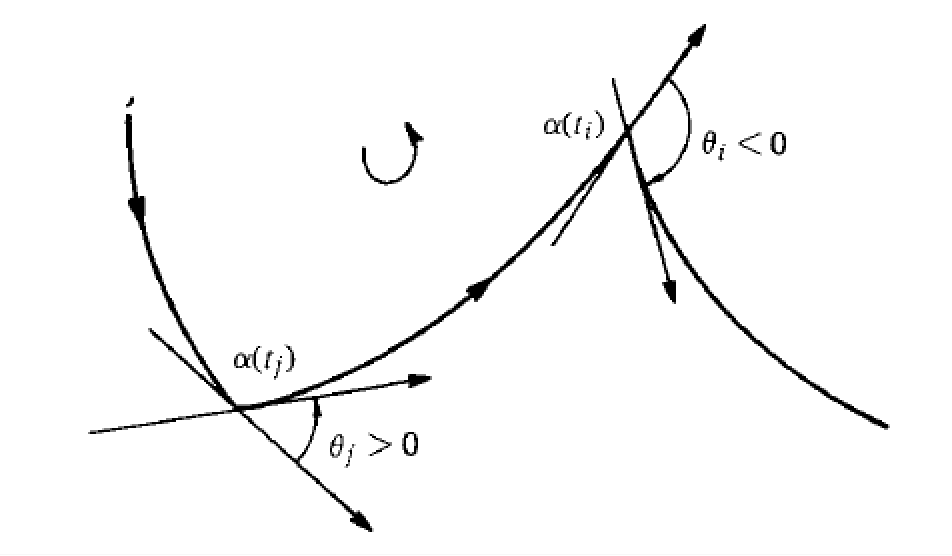
\includegraphics[scale = 0.43]{external_angle.png}}
 \caption{\scriptsize{\textbf{ The external angle $\theta_{i}$ at vertex $\alpha(t_{i})$ }}}\label{fig: external_angle}
\end{figure}

\end{definition}


\item \begin{theorem} (The Global Gauss-Bonnet theorem):\\
Let $R\subset \cS$ be a regular region of an oriented surface $\cS$ and let $\cC_{1}, \ldots, \cC_{n}$ be the closed, simple, piecewise regular curves which form the boundary of $R$, $\partial R$. Suppose that each $\cC_{i}$ is positively oriented and let $\theta_{1},\ldots, \theta_{p}$ be the set of all \emph{external} angles of the curves $\cC_{1}, \ldots, \cC_{n}$. Then
\begin{align*}
\sum_{i=1}^{n}\int_{\cC_{i}}k_{g}(s)ds + \iint_{R}\mb{K}d\mb{\sigma} + \sum_{m=1}^{p}\theta_{m} &= 2\pi \;\chi(R)
\end{align*} 
where $s$ denotes the arc length of $\cC_{i}$ and the integral over $\cC_{i}$ means that the sum of integrals in every regular arc of $\cC_{i}$. The integral 
\begin{align*}
\iint_{R}\mb{K}d\mb{\sigma} 
\end{align*} means the integral over a regular region. 
\end{theorem}

\item \begin{corollary}
Let $T$ be a geodesic triangle in an oriented surface $\cS$. Let $\theta_{1}, \theta_{2}, \theta_{3}$ be external angles of $T$ and let $\phi_{i}= \pi- \theta_{i}$, $1\le i\le 3$ be the interior angles. Then 
\begin{align*}
\iint_{T}\mb{K}d\mb{\sigma} +  \sum_{i=1}^{3}\theta_{i} = 2\pi &&\Leftrightarrow \iint_{T}\mb{K}d\mb{\sigma}= \sum_{i=1}^{3}\phi_{i} - \pi.
\end{align*} 
\begin{figure}[htb]
\centering
 \centerline{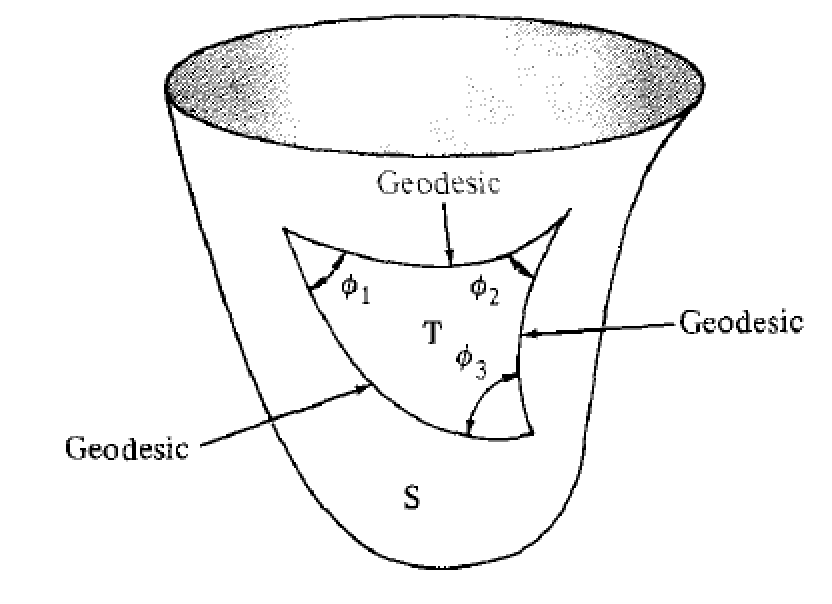
\includegraphics[scale = 0.4]{Gauss_Bonnet_triangle.png}}
 \caption{\scriptsize{\textbf{Since the sum of interior angles is not $\pi$, it indicates that the geometry of the surface is non-Euclidean. }}}\label{fig: external_angle}
\end{figure}
\end{corollary}
\end{itemize}

\newpage
\section{Computational tools and formulas}
\subsection{algebra and calculus}
\begin{itemize}
\item The cross product (vector product) of two vectors $\mb{u}$ and $\mb{v}$ under the basis $\set{\mb{e}_{1}, \mb{e}_{2}, \mb{e}_{3}}$ is denoted as $\mb{u}\wedge \mb{v}$ and computed as
\begin{align}
\inn{\mb{u}\wedge \mb{v}}{\mb{w}} &= \det\abs{\begin{array}{ccc}
u_{1} & u_{2} & u_{3} \\ 
v_{1} & v_{2} & v_{3} \\ 
w_{1} & w_{2} & w_{3}
\end{array} }  \equiv \det(\mb{u, v, w})\label{eqn: cross_prod}
\end{align}
and
\begin{align}
\mb{u}\wedge \mb{v} \equiv \mb{u} \times \mb{v} &\equiv \abs{\begin{array}{cc}
u_{2} & u_{3} \\ 
v_{2} & v_{3}
\end{array} }\mb{e}_{1}
- 
\abs{\begin{array}{cc}
u_{1} & u_{3} \\ 
v_{1} & v_{3}
\end{array} }\mb{e}_{2}
+
\abs{\begin{array}{cc}
u_{1} & u_{2} \\ 
v_{1} & v_{2}
\end{array} }\mb{e}_{3}  \label{eqn: cross_prod2}
\end{align}

\end{itemize}

\subsection{curves}
\begin{itemize}
\item The \emph{arc length} of a regular parameterized curve $\alpha: I \rightarrow \bR^{3}$ from $t_{0}$ is defined as
\begin{align}
s &\equiv \int_{t_{0}}^{t}\abs{\alpha'(t)} dt  \label{eqn: arc_leng_1}
\end{align} where $\abs{\alpha'(t)} = \sqrt{(x'(t))^{2} + (y'(t))^{2}+ (z'(t))^{2}}$.

\item The curvature $k(s) \equiv \abs{\alpha''(s)}$.

\item The Frenet trihedron $(\mb{t}, \mb{n}, \mb{b})$ at $s$ can be computed via the system of differential equations as 
\begin{align}
\mb{t}' &= k\,\mb{n}\nonumber\\
\mb{n}' &= -k\,\mb{t} - \tau\,\mb{b}\nonumber\\
\mb{b}' &= \tau\,\mb{n} \label{eqn: Frenet_formula}
\end{align}
called \emph{Frenet formula} \citep{do1976differential}, where $k(s)>0$ and $\tau(s)$ are the curvature and torsion of a regular parameterized curve, respectively.  

From theorem \ref{th: curv_tri}, we see that the curvature and torsion function determine a parameterized regular curve up to a rigid transformation.  It is thus called \emph{the fundamental theorem of the local theory of curves}.
\end{itemize}
\subsection{surfaces}
\begin{itemize}
\item (Tangent vector via basis)\\
 For $\alpha'(0)\equiv \mb{w} \in T_{p}S$, for some $\alpha = \mb{x}\circ \mb{\beta}$, where $\mb{\beta}: (-\epsilon, \epsilon) \rightarrow U$ by $\mb{\beta}(t) = (u(t), v(t))$, with $\mb{\beta}(0) = q = \mb{x}^{-1}(p)$. Then 
\begin{align}
\alpha'(0)&= \frac{d}{dt}(\mb{x}\circ\mb{\beta})(0) = \frac{d}{dt}\mb{x}(u(t), v(t))(0)\\
&=\mb{x}_{u}u'(0) + \mb{x}_{v}v'(0) \label{eqn: tangent_line_coord}
\end{align} 
Thus under the basis $(\mb{x}_{u}, \mb{x}_{v})$ of $T_{p}S$, the coordinate of $\mb{w}$ in $T_{p}S$ is $(u'(0), v'(0))$, and $\mb{w}$ is the velocity of  the curve $\alpha$ is represented as $(u(t), v(t))$ in parameterization $\mb{x}$ at $t=0$. 

\item (Differential of map via basis)\\
 If $\mb{w} = (u'(0), v'(0))$ in $T_{p}(S_{1})$,  and $\varphi(u,v) = (\varphi_{1}(u,v), \varphi_{2}(u,v))$, with $\alpha(t) = (u(t), v(t))$, then the tangent of $\beta$ at $\varphi(p)$ is given via the differential of map of $\mb{w}$ at $p$ is given in its own coordinates as 
\begin{align}
 \beta'(0)= d\varphi_{p}(\mb{w}) &= \brac{\begin{array}{cc}
 \dpartdiff{\varphi_{1}}{u} & \dpartdiff{\varphi_{1}}{v} \\ 
 \dpartdiff{\varphi_{2}}{u} & \dpartdiff{\varphi_{2}}{v}
 \end{array} } \brac{\begin{array}{c}
 u'(0) \\ 
 v'(0)
 \end{array} } \label{eqn: diff_map_coord}
\end{align}
Thus $d\varphi_{p}$ as a linear mapping under coordinates $(\mb{x}_{u}, \mb{x}_{v})$ in $T_{p}S$ and $(\mb{x}^{'}_{u'}, \mb{x}^{'}_{v'})$ in $T_{p}S$ is given as the matrix $\brac{\begin{array}{cc}
 \partdiff{\varphi_{1}}{u} & \partdiff{\varphi_{1}}{v} \\ 
 \partdiff{\varphi_{2}}{u} & \partdiff{\varphi_{2}}{v}
 \end{array} } $.
 
 \item Given a parameterization $\mb{x}: U\subset \bR^{2} \rightarrow \cS$, the normal vector $N(p)$ at $p$ is given via
\begin{align}
N(p) &= \frac{\mb{x}_{u} \wedge \mb{x}_{v}}{\abs{\mb{x}_{u} \wedge \mb{x}_{v}}}(p) \label{eqn: normal_vec_field_1}
\end{align}

\item The \emph{first fundamental form} of a regular surface $\cS\subset \bR^{3}$ at $p\in \cS$ is defined as a  quadratic form,  $I_{p}: T_{p}S \rightarrow \bR$ given by 
\begin{align}
I_{p}(\mb{w}) &= \inn{w}{w}_{p} = \norm{w}{2}^{2} \ge 0\; \; \mb{w}\in T_{p}S. \label{eqn: first_fund_form1}
\end{align}

\item (The first fundamental form via basis)\\
Under the basis $\set{\mb{x}_{u}, \mb{x}_{v}}$ associated with $\mb{x}(u,v)$ at $p$, the first fundamental form can be formulated explicitly. Since $\mb{w} = \alpha'(0)$ for $\alpha:  (-\epsilon, \epsilon) \rightarrow \cS$ with $\alpha(t) = (u(t), v(t))$ and $p = \alpha(0) = \mb{x}(u(0), v(0))$, thus
\begin{align}
I_{p}(\alpha'(0)) &= \inn{\mb{x}_{u}u'(0) + \mb{x}_{v}v'(0)}{\mb{x}_{u}u'(0) + \mb{x}_{v}v'(0)} \nonumber\\
&= \inn{\mb{x}_{u}}{\mb{x}_{u}}\paren{u'(0)}^{2} + 2\,\inn{\mb{x}_{u}}{\mb{x}_{v}}\paren{u'(0)v'(0)} +  \inn{\mb{x}_{v}}{\mb{x}_{v}}\paren{v'(0)}^{2}\nonumber\\
&= E\,\paren{u'(0)}^{2} + 2\,F\paren{u'(0)v'(0)} + G\paren{v'(0)}^{2} \label{eqn: first_fund_form2}
\end{align}
and 
\begin{align}
E(u(0), v(0)) &= \inn{\mb{x}_{u}}{\mb{x}_{u}}_{p}\nonumber\\
F(u(0), v(0)) &= \inn{\mb{x}_{u}}{\mb{x}_{v}}_{p}\nonumber\\
G(u(0), v(0)) &= \inn{\mb{x}_{v}}{\mb{x}_{v}}_{p} \label{eqn: first_fund_coeff}
\end{align} are \emph{coefficients of the first fundamental form} in the basis $\set{\mb{x}_{u}, \mb{x}_{v}}$. Note that $p=\mb{x}(u,v)$ runs in the coordinate neighborhood, the quantities $E(u,v), F(u,v), G(u,v)$ are differentiable function on $U$.

The matrix of first fundamental form is given as 
\begin{align}
\mb{J}\equiv \brac{\begin{array}{cc}
\inn{\mb{x}_{u}}{\mb{x}_{u}}_{p} &  \inn{\mb{x}_{u}}{\mb{x}_{v}}_{p} \\ 
 \inn{\mb{x}_{v}}{\mb{x}_{u}}_{p} & \inn{\mb{x}_{v}}{\mb{x}_{v}}_{p}
\end{array} } = 
\brac{\begin{array}{cc}
E & F \\ 
F & G
\end{array} } \label{eqn: first_fund_form3}
\end{align}
and for $\mb{w} = \alpha'(0) = (u'(0), v'(0))$, 
\begin{align*}
I_{p}(\mb{w}) &= \mb{w}^{T}\,\mb{J}\,\mb{w}
\end{align*}\\

\item Given the first fundamental form $I(\alpha'(t))$ on $T_{p}S$, we can evaluate the the arc length without using its coordinate in $\bR^{3}$ 
\begin{align}
s &= \int_{0}^{t} \sqrt{I(\alpha'(t))}  dt\nonumber\\
&= \int_{0}^{t} \sqrt{E(u'(t))^{2}+ 2\,F\,(u'(t)v'(t)) + G\,(v'(t))^{2}  }  dt \nonumber\\
&=  \int_{0}^{t} \sqrt{ \dpartdiff{\mb{\alpha}}{t}^{T}\mb{J}\, \dpartdiff{\mb{\alpha}}{t} }  dt  \label{eqn: arc_leng_2}
\end{align}

\item Also, we can compute the angle btw two parameterized regular curve $\alpha(t)$ and $\beta(t)$ on $\cS$ that intersects at $t=t_{0}$ as 
\begin{align*}
\cos(\theta) &= \frac{\inn{\alpha'(t_{0})}{\beta'(t_{0})}}{\norm{\alpha'(t_{0})}{2}\,\norm{\beta'(t_{0})}{2}}.
\end{align*}
Then the angle $\phi$ btw two coordinate curves of a parameterization $\mb{x}(u,v)$ is given by 
\begin{align*}
\cos(\phi) &= \frac{\inn{\mb{x}_{u}}{\mb{x}_{v}}}{\norm{\mb{x}_{u}}{2}\,\norm{\mb{x}_{v}}{2}} = \frac{F}{\sqrt{E\,G}}.
\end{align*}

\item The \emph{area} for a bounded region $\cR$ of a regular surface $\cS$ in the coordinate neighborhood of a parameterization $\mb{x}(u,v)$ is given as 
\begin{align}
\int\int_{Q} \abs{\mb{x}_{u}\wedge \mb{x}_{v}}dudv, \quad Q = \mb{x}^{-1}(\cR) \label{eqn: area_first_fund}
\end{align} 
where $\abs{\mb{x}_{u}\wedge \mb{x}_{v}} = \sqrt{EG - F^{2}}$.
\end{itemize}

\subsection{Gauss map}
\begin{itemize}
\item (Differential of normal vector field under basis)\\
For $p\in \cS$, $dN_{p}: T_{p}S \rightarrow T_{p}S$ is a linear transformation in $T_{p}S$. Let $\alpha(t) = \mb{x}(u(t), v(t))$ be a parameterized regular curve on surface $\cS$ with the tangent vector $\alpha'(t) = \mb{x}_{u}u'(t) + \mb{x}_{v}v'(t) $ under the basis $\set{\mb{x}_{u}, \mb{x}_{v}}$. Then 
\begin{align}
dN_{p}(\alpha'(t)) &= dN_{p}( \mb{x}_{u}u'(t) + \mb{x}_{v}v'(t) )\nonumber\\
&= \dfrac{d}{dt}N\paren{u(t), v(t)} = N_{u}u'(t) + N_{v}v'(t), \label{eqn: Gauss_map}
\end{align} where $N_{u} = dN_{p}( \mb{x}_{u})$ and  $N_{v} = dN_{p}( \mb{x}_{v})$. Note that $N_{u} \in T_{p}S$ and $N_{v} \in T_{p}S$, therefore
\begin{align}
N_{u}&= a_{11}\mb{x}_{u} + a_{21}\mb{x}_{v}\nonumber\\
N_{v}&= a_{12}\mb{x}_{u} + a_{22}\mb{x}_{v}. \label{eqn: Gauss_map_comp}
\end{align}
Note that $N(t) = N\circ \alpha(t)$ is a line on the unit sphere and $dN_{p}(\alpha') = N'(t)$ on the unit sphere. 

Under the basis $\set{\mb{x}_{u}, \mb{x}_{v}}$, 
\begin{align}
dN_{p}\,\paren{\begin{array}{c}
u'(t)  \\ 
v'(t) 
\end{array} } &= 
\brac{\begin{array}{cc}
a_{11} & a_{12} \\ 
a_{21} & a_{22}
\end{array} }\paren{\begin{array}{c}
u'(t)  \\ 
v'(t) 
\end{array} }  \label{eqn: Gauss_map_coord}
\end{align}
Note that if $\set{\mb{x}_{u}, \mb{x}_{v}}$ is not orthonormal, the above matrix $[a_{i,j}]$ is not necessary symmetric. \\


\item The quadratic form $\Pi_{p}$ defined in $T_{p}S$ by $\Pi_{p}(\mb{v}) = -\inn{dN_{p}(\mb{v})}{\mb{v}}$ is called the \emph{second fundamental form} of $\cS$ at $p$.

\item Given the principal curvature at $p$, one can compute the normal curvature $k_{n}$ at $p$ along any direction $\mb{v}\in T_{p}S$ with $\norm{\mb{v}}{} = 1$, as $\mb{v} = \mb{e}_{1}\cos(\theta) + \mb{e}_{2}\sin(\theta)$, where $\theta$ is the angle from $\mb{e}_{1}$ to $\mb{v}$. Hence
\begin{align}
k_{n} &= \Pi_{p}(\mb{v}) = -\inn{dN_{p}(\mb{v})}{\mb{v}}\nonumber\\
&= -\inn{dN_{p}( \mb{e}_{1}\cos(\theta) + \mb{e}_{2}\sin(\theta))}{ \mb{e}_{1}\cos(\theta) + \mb{e}_{2}\sin(\theta)}\nonumber\\
&= \inn{k_{1}\mb{e}_{1}\cos(\theta) + k_{2}\mb{e}_{2}\sin(\theta)}{\mb{e}_{1}\cos(\theta) + \mb{e}_{2}\sin(\theta)}\nonumber\\
&= k_{1}\cos(\theta)^{2} + k_{2}\sin(\theta)^{2}. \label{eqn: Euler_formula}
\end{align}
The above formula is called the \emph{Euler formula}. This is the formula for the second fundamental form in the basis $\set{\mb{e}_{1}, \mb{e}_{2}}$ induced by the principal directions. 

\item  (Dupin indicatrix under basis)\\
Let $(\mb{e}_{1}, \mb{e}_{2})$ be the basis of $T_{p}S$ as the principal directions of $dN_{p}$. Then via a polar coordinate $\mb{w} = \rho\,\mb{v}$ and $\mb{v} = \xi\mb{e}_{1}+ \eta\mb{e}_{2}$. By Euler's formula, the Dupin indicatrix satisfies the following equation
 \begin{align*}
 \pm 1 = \Pi_{p}(\mb{w}) &= \rho^{2}\,\Pi_{p}(\mb{v})\\
 &= k_{1}\rho^{2}\cos^{2}(\theta) + k_{2}\rho^{2}\sin^{2}(\theta) \\
 &= k_{1}\xi^{2} + k_{2}\eta^{2}.
 \end{align*}
Thus the set of coordinates $(\xi, \eta)$ satisfies the Dupin indicatrix is the a union of conics in $T_{p}S$. The normal curvature along the direction $\mb{w}$ is $k_{n}(\mb{v}) = \pm \frac{1}{\rho^{2}}$.

It is clear that for an \emph{elliptic point}, the Dupin indicatrix is an \emph{ellipse}, i.e. $k_{1}\xi^{2} + k_{2}\eta^{2} = 1$. 

For an \emph{hyperbolic point}, the Dupin indicatrix is made of \emph{two hyperbolas with a common pair of asymptotic lines}, i.e. i.e. $k_{1}\xi^{2} + k_{2}\eta^{2} = -1$. Along the direction of asymptotes, the normal curvature is zero; they are therefore the asymptotic directions. A hyperbolic point has exactly two asymptotic directions.  

For a \emph{parabolic point}, the Dupin indicatrix degenerates into a pair of \emph{parallel lines} as one of the principal curvature is zero. The common direction of these lines is the only asymptotic directions at the given point. \\


\item (The second fundamental form under basis)\\
Given the basis $\set{\mb{x}_{u}, \mb{x}_{v}}$ in $T_{p}S$ at $p\in \cS$, and let $\alpha(t) = \mb{x}(u(t), v(t))$ be a parameterized regular curve on surface $\cS$ with the tangent vector $\alpha'(t) = \mb{x}_{u}u'(t) + \mb{x}_{v}v'(t) $ under the basis $\set{\mb{x}_{u}, \mb{x}_{v}}$ and $p=\alpha(0)= \mb{x}(u(0), v(0))$. The second fundamental form is computed as
\begin{align}
\Pi_{p}(\alpha') &=  -\inn{dN_{p}(\alpha')}{\alpha'}\nonumber\\
&= -\inn{N_{u}u'(t) + N_{v}v'(t)}{ \mb{x}_{u}u'(t) + \mb{x}_{v}v'(t)}\nonumber\\
&= e\paren{u'(t)}^{2} + 2f\paren{u'(t)v'(t)} + g\paren{v'(t)}^{2} \label{eqn: second_fund_form_2}
\end{align}
where the coefficient for the second fundamental form is given as 
\begin{align}
e(u(0), v(0))&= - \inn{N_{u}}{\mb{x}_{u}} = \inn{N}{\mb{x}_{uu}} \nonumber\\
f(u(0), v(0))&= - \inn{N_{u}}{\mb{x}_{v}} =  \inn{N}{\mb{x}_{vu}} =  \inn{N}{\mb{x}_{uv}} =  -\inn{N_{v}}{\mb{x}_{u}}\nonumber\\
g(u(0), v(0))&=   - \inn{N_{v}}{\mb{x}_{v}} = \inn{N}{\mb{x}_{vv}}  \label{eqn: second_fund_coeff}
\end{align}
and the last equality in each row comes by differentiating both equations $\inn{N}{\mb{x}_{u}} = 0$ and $\inn{N}{\mb{x}_{v}} = 0$ with respect to either $u$ or $v$, respectively. 

We can compute these coefficients from $\set{\mb{x}_{uu},\mb{x}_{uv}, \mb{x}_{vv}, N }$. In specific, by using the formula in \eqref{eqn: cross_prod}, \eqref{eqn: normal_vec_field_1} and \eqref{eqn: second_fund_coeff}
\begin{align}
e &= \inn{N}{\mb{x}_{uu}} = \inn{\frac{\mb{x}_{u} \wedge \mb{x}_{v}}{\abs{\mb{x}_{u} \wedge \mb{x}_{v}}}}{\mb{x}_{uu}}= \frac{\det\paren{ \mb{x}_{u} , \mb{x}_{v}, \mb{x}_{uu}  }}{EG- F^{2}} \nonumber\\
f &= \inn{N}{\mb{x}_{uv}} = \inn{\frac{\mb{x}_{u} \wedge \mb{x}_{v}}{\abs{\mb{x}_{u} \wedge \mb{x}_{v}}}}{\mb{x}_{uv}}= \frac{\det\paren{ \mb{x}_{u} , \mb{x}_{v}, \mb{x}_{uv}  }}{EG- F^{2}} \nonumber\\
g &= \inn{N}{\mb{x}_{uu}} = \inn{\frac{\mb{x}_{u} \wedge \mb{x}_{v}}{\abs{\mb{x}_{u} \wedge \mb{x}_{v}}}}{\mb{x}_{vv}}= \frac{\det\paren{ \mb{x}_{u} , \mb{x}_{v}, \mb{x}_{vv}  }}{EG- F^{2}} \label{eqn: second_fund_coeff_2}
\end{align}



By the matrix $[a_{i,j}]$ in \eqref{eqn: Gauss_map_coord}, and the coefficient for the first fundamental form in \eqref{eqn: first_fund_coeff}, 
\begin{align}
-f &=  \inn{N_{u}}{\mb{x}_{v}} = \inn{a_{11}\mb{x}_{u} + a_{21}\mb{x}_{v}}{\mb{x}_{v}} = a_{11}F + a_{21}G, \nonumber\\
-f &=  \inn{N_{v}}{\mb{x}_{u}} = \inn{a_{12}\mb{x}_{u} + a_{22}\mb{x}_{v}}{\mb{x}_{u}} = a_{12}E + a_{22}F, \nonumber\\
-e &= \inn{N_{u}}{\mb{x}_{u}}  = \inn{a_{11}\mb{x}_{u} + a_{21}\mb{x}_{v}}{\mb{x}_{u}} = a_{11}E + a_{21}F, \nonumber\\
-g &= \inn{N_{v}}{\mb{x}_{v}}  = \inn{a_{12}\mb{x}_{u} + a_{22}\mb{x}_{v}}{\mb{x}_{v}} = a_{12}F + a_{22}G. \label{eqn: second_fund_coeff_3} 
\end{align}
From \eqref{eqn: second_fund_coeff_3}, in matrix form, we have
\begin{align}
-\brac{\begin{array}{cc}
e & f \\ 
f & g
\end{array} }
&= 
\brac{\begin{array}{cc}
a_{11} & a_{21} \\ 
a_{12} & a_{22}
\end{array} }
\brac{\begin{array}{cc}
E & F \\ 
F & G
\end{array} }
\end{align}
One can compute the coefficients $[a_{i,j}]$ as
\begin{align*}
\brac{\begin{array}{cc}
a_{11} & a_{21} \\ 
a_{12} & a_{22}
\end{array} }
&= -\brac{\begin{array}{cc}
e & f \\ 
f & g
\end{array} }
\brac{\begin{array}{cc}
E & F \\ 
F & G
\end{array} }^{-1}
\end{align*} or
\begin{align}
a_{11} &= \frac{fF- eG}{EG- F^{2}} \nonumber\\
a_{12} &= \frac{gF- fG}{EG- F^{2}} \nonumber\\
a_{21} &= \frac{eF- fE}{EG- F^{2}} \nonumber\\
a_{22} &= \frac{fF- gE}{EG- F^{2}} \label{eqn: weingarten}
\end{align}
which is called the \emph{equations of Weingarten}. 

\item Given the coefficients for the second fundamental form $(e,f,g)$ and those for the first fundamental form $(E,F,G)$, the \emph{Gaussian curvature} can be computed as 
\begin{align}
\mb{K} &= \det\brac{a_{i,j}} = \frac{eg- f^{2}}{EG- F^{2}} \label{eqn: Gaussian_curvature}
\end{align}

\item 
The principal curvature $(k_{1}, k_{2})$ is the eigenvalue of $-dN_{p}$, which is the solution of equations
\begin{align*}
\det\brac{\begin{array}{cc}
a_{11}+ k & a_{12} \\ 
a_{21} & a_{22}+k
\end{array} } = 0
\end{align*} or
\begin{align*}
k^{2}+ k(a_{11}+ a_{22}) + a_{11}a_{22} - a_{12}a_{21} = 0
\end{align*}
\begin{align}
k &= \mb{H} \pm \sqrt{\mb{H}^{2}- \mb{K}}  \label{eqn: principal_curv_coord}
\end{align}
where the \emph{mean curvature} is 
\begin{align}
\mb{H} &= -\frac{1}{2}(a_{11}+ a_{22}) = \frac{1}{2}\frac{eG - 2fF + gE}{EG-F^{2}}
\end{align}


\item (Asymptotic directions under basis)\\
A connected regular curve $\cC$ in the coordinate neighborhood of $\mb{x}$ as $\alpha(t) = \mb{x}(u(t), v(t)), t\in I$ is an \emph{asymptotic curve} iff $\Pi(\alpha'(t)) = 0$ for all $t\in I$. Then it follows that
\begin{align}
e(u')^{2} + 2f(u'v') + g(v')^{2} = 0,\quad t\in I \label{eqn: diff_eqn_asym_curve}
\end{align}
is called the \emph{differential equation for the asymptotic curves}. 

A direct conclusion from \eqref{eqn: diff_eqn_asym_curve} is that for the \emph{hyperbolic point} $p\in \cC\subset \cS$, a necessary and sufficient condition for a parameterization $\mb{x}$ in its neighborhood to be such that the coordinate curves of the parameterization are asymptotic curves is that $e= g= 0$.

\item (Principal directions under basis)\\
A connected regular curve $\cC$ the coordinate neighborhood of $\mb{x}$ as $\alpha(t) = \mb{x}(u(t), v(t)), t\in I$ is a \emph{line of curvature} iff for any paramterization $\mb{x}$, we have 
\begin{align*}
dN(\alpha'(t)) &= \lambda(t)\alpha'(t)
\end{align*}
Thus
\begin{align*}
\brac{\begin{array}{cc}
a_{11} & a_{21} \\ 
a_{12} & a_{22}
\end{array} }\brac{\begin{array}{c}
u' \\ 
v'
\end{array} } &= \lambda\,\brac{\begin{array}{c}
u' \\ 
v'
\end{array} }
\end{align*}
Thus by \eqref{eqn: weingarten} and eliminating $\lambda$, we have
\begin{align}
&(fE- eF)(u')^{2} + (gE-eG)(u'v')+ (gF-fG)(v')^{2} = 0\nonumber\\[5pt]
\text{or }& 
\det\abs{\begin{array}{ccc}
(v')^{2} & -(u'v') & (u')^{2}  \\ 
E & F & G \\ 
e & f & g
\end{array} } = 0, \label{eqn: diff_eqn_line_curvature}
\end{align} which is called the \emph{differential equation for the lines of curvature}.

Note that the principal directions are orthogonal to each other $(u'v' =0)$, it concludes from \eqref{eqn: diff_eqn_line_curvature} that a necessary and sufficient condition for the coordinate curves of a parameterization to be lines of curvature in a neighborhood of a nonumbilical point is that $F=f = 0$. 
\end{itemize}

\subsection{Intrinsic geometry of surfaces}
\begin{itemize}
\item (The representation of partial derivatives of basis under basis)\\
Note that given parameterization $\mb{x}: U \rightarrow \cS$ and a point $p\in \cS$, the trihedron $(\mb{x}_{u}, \mb{x}_{v}, N)$ at $p$ form a basis in ambient space. In terms of this, the partial derivatives of these basis vector in this space can be linearly represented by this basis, i.e. 
\begin{align}
\partdiff{\mb{x}_{u}}{u} = \mb{x}_{uu} &= \Gamma_{11}^{1}\mb{x}_{u} +  \Gamma_{11}^{2}\mb{x}_{v} + e\,N\nonumber\\
\partdiff{\mb{x}_{u}}{v} = \mb{x}_{uv} &= \Gamma_{12}^{1}\mb{x}_{u} +  \Gamma_{12}^{2}\mb{x}_{v} + f\,N\nonumber\\
\partdiff{\mb{x}_{v}}{u} = \mb{x}_{vu} &= \Gamma_{21}^{1}\mb{x}_{u} +  \Gamma_{21}^{2}\mb{x}_{v} + f\,N\nonumber\\
\partdiff{\mb{x}_{v}}{v} = \mb{x}_{vv} &= \Gamma_{22}^{1}\mb{x}_{u} +  \Gamma_{22}^{2}\mb{x}_{v} + g\,N\nonumber\\
\partdiff{N}{u} =N_{u} &= a_{11}\mb{x}_{u} +  a_{21}\mb{x}_{v} \nonumber\\
\partdiff{N}{v} =N_{v} &= a_{12}\mb{x}_{u} +  a_{22}\mb{x}_{v} \label{eqn: Christoffel_eq_1}
\end{align}

The coefficients $\Gamma_{i,j}^{k}$ for $i,j,k = 1,2$ are called \emph{Christoffel symbols} of $\cS$ in paramterization. It is  a function of intrinsic parameters. From \eqref{eqn: Christoffel_eq_1}, it is seen that the Christoffel symbols are linear coefficients of the projection of $\mb{x}_{uu}, \mb{x}_{uv}, \mb{x}_{vv}$ onto the tangent plane of the surface, whereas their normal complements are represented via $e,f,g$, the coefficients of second fundamental form. The coefficients $[a_{i,j}]$ determines the differential of Gauss map $dN_{p}$, which is a function of first fundamental form $E,F,G$. 

Like Frenet formula in \eqref{eqn: Frenet_formula}, the above formula \eqref{eqn: Christoffel_eq_1} is \emph{the fundamental theorem of the local theory of surfaces}. 



\item (Christoffel symbols via coefficients of first fundamental form)\\
The Christoffel symbols can be determined by taking the inner product of the first four equations in \eqref{eqn: Christoffel_eq_1} with $\mb{x}_{u}$ and $\mb{x}_{v}$, i.e. 
\begin{align}
&\left\{ \begin{array}{ccl}
\Gamma_{11}^{1}E + \Gamma_{11}^{2}F &= \inn{\mb{x}_{uu}}{\mb{x}_{u}} &= \frac{1}{2}E_{u} \\ 
\Gamma_{11}^{1}F + \Gamma_{11}^{2}G &= \inn{\mb{x}_{uu}}{\mb{x}_{v}} &= F_{u} - \frac{1}{2}E_{v} 
\end{array} \right. \nonumber\\
&\left\{ \begin{array}{ccl}
\Gamma_{12}^{1}E + \Gamma_{12}^{2}F &= \inn{\mb{x}_{uv}}{\mb{x}_{u}} &= \frac{1}{2}E_{v} \\ 
\Gamma_{12}^{1}F + \Gamma_{12}^{2}G &= \inn{\mb{x}_{uv}}{\mb{x}_{v}} &= \frac{1}{2}G_{u}  
\end{array} \right. \nonumber\\
&\left\{ \begin{array}{ccl}
\Gamma_{22}^{1}E + \Gamma_{22}^{2}F &= \inn{\mb{x}_{vv}}{\mb{x}_{u}} &=F_{v} - \frac{1}{2}G_{u}  \\ 
\Gamma_{22}^{1}F + \Gamma_{22}^{2}G &= \inn{\mb{x}_{vv}}{\mb{x}_{v}} &= \frac{1}{2}G_{v}   
\end{array} \right. \label{eqn: Christoffel_eq_2}
\end{align}
There are three pairs of equations and each pair uniquely determines a pair of Christoffel symbol $(\Gamma_{i,j}^{1}, \Gamma_{i,j}^{2}), i,j=1,2$. \emph{This system of equations in \eqref{eqn: Christoffel_eq_2} determines the Christoffel symbol only in terms of the coefficients of first fundamental form $(E,F,G)$}.  

Note that $\Gamma_{i,j}^{k} = \Gamma_{j,i}^{k}$, i.e. the Chrisoffel symbol is symmetric w.r.t. the lower indices.

In particular, for orthogonal parameterization, $F=0$, the Christoffel symbol can be computed as
\begin{align*}
\Gamma_{11}^{1} &= \frac{1}{2}\frac{E_{u}}{E};  &
\Gamma_{11}^{2} &= -\frac{1}{2}\frac{E_{v}}{G};\\
\Gamma_{12}^{1} &= \frac{1}{2}\frac{E_{v}}{E};  &
\Gamma_{12}^{2} &= \frac{1}{2}\frac{G_{u}}{G};\\
\Gamma_{22}^{1} &= -\frac{1}{2}\frac{G_{u}}{E};  &
\Gamma_{22}^{2} &= \frac{1}{2}\frac{G_{v}}{G}.
\end{align*}
\\

\item (The linear relationship between coefficients of first and second fundamental forms)\\
The relationship btw coefficients of first and second fundamental forms can be computed via the following equations
\begin{align}
\paren{\mb{x}_{uu}}_{v} - \paren{\mb{x}_{uv}}_{u} = 0\nonumber\\
\paren{\mb{x}_{vv}}_{u} - \paren{\mb{x}_{uv}}_{v} = 0\nonumber\\
N_{uv} - N_{vu} = 0\label{eqn: coeff_12_fund_relation_1}
\end{align}
By substituting \eqref{eqn: Christoffel_eq_1}, it equals to 
\begin{align}
A_{1}\mb{x}_{u} + B_{1}\mb{x}_{v} + C_{1}N = 0\nonumber\\
A_{2}\mb{x}_{u} + B_{2}\mb{x}_{v} + C_{2}N = 0\nonumber\\
A_{3}\mb{x}_{u} + B_{3}\mb{x}_{v} + C_{3}N = 0\label{eqn: coeff_12_fund_relation_2} 
\end{align}
where $A_{i}, B_{i}, C_{i}, i=1,2,3$ are functions of $e,f,g,E,F,G$ and of their derivatives. By linearly independence of $(\mb{x}_{u}, \mb{x}_{v}, N)$, it yields nine equations
\begin{align}
A_{i} =0; \quad B_{i} = 0; \quad C_{i}=0 \quad i=1,2,3,  \label{eqn: comp_eqn_1}
\end{align} This system of equations are related to the \emph{compatibility equations} of the theory of surfaces. 

\item By solving the equations \eqref{eqn: comp_eqn_1}, one obtain the following equations
\begin{align}
\paren{\Gamma_{12}^{2}}_{u}- \paren{\Gamma_{11}^{2}}_{v} - \Gamma_{11}^{1}\Gamma_{12}^{2} - \Gamma_{11}^{2}\Gamma_{22}^{2} + \Gamma_{12}^{1}\Gamma_{11}^{2} +\paren{\Gamma_{12}^{2}}^{2}
&= -\mb{K}E \nonumber\\
\paren{\Gamma_{12}^{1}}_{u}-\paren{\Gamma_{11}^{1}}_{v} -   \Gamma_{11}^{2}\Gamma_{22}^{1}  + \Gamma_{12}^{2}\Gamma_{12}^{1}
&= \mb{K}F \nonumber\\
 e\Gamma_{12}^{1} + f(\Gamma_{12}^{2} - \Gamma_{11}^{1}) - g\Gamma_{11}^{2}&= e_{v} - f_{u}  \nonumber\\
 e\Gamma_{22}^{1} + f(\Gamma_{22}^{2} - \Gamma_{12}^{1}) - g\Gamma_{12}^{2}&= f_{v} - g_{u},  \label{eqn: comp_eqn_surface_formula}
\end{align} 
where $\mb{K}$ is the Gaussian curvature shown in Gaussian theorem. The first two equations are called the \emph{Gauss formula} and the last two equations are called the \emph{Mainardi-Codazzi equations}.  These four equations are known as the \emph{compatibility equations of the theory of surfaces}. 
\end{itemize}
\subsection{Functions on manifold}
\begin{itemize}
\item For $T_{p}\cM = \text{span}\set{ \rlat{\partdiff{}{x_{i}}}{p},\; 1\le i\le V}$, the dual space $T^{*}_{p}\cM= \text{span}\set{ \rlat{\lambda_{i}}{p},\; 1\le i\le V}$. For any $\omega \in T^{*}_{p}\cM$, $\omega =\sum_{i} \omega_{i}\lambda_{i}$ with 
\begin{align*}
\omega_{i} &= \omega\paren{\rlat{\partdiff{}{x_{i}}}{p}}.
\end{align*}

\item Let $f: \cM \rightarrow \bR$ be a smooth function on manifold $\cM$. The \emph{(covariant) differential} of $f$ at $p\in \cM$, $df: T_{p} \rightarrow \bR$ is a linear mapping. It is given by 
\begin{align*}
df_{p}(\mb{w}(p)) &= \mb{w}(p)f, \quad \mb{w}(p) \in T_{p}\cM.
\end{align*} for vector field $\mb{w}$. Note that $\mb{w}(p)f= (w_{i}(p)\partdiff{}{x_{i}})f=w_{i}(p)\partdiff{}{x_{i}}f$.

The differential map is decomposed as
\begin{align*}
df_{p} &= \sum_{i} \partdiff{f}{x_{i}}(p)\rlat{\lambda_{i}}{p} \equiv \sum_{i} \partdiff{f}{x_{i}}(p)\rlat{dx_{i}}{p}\\
\end{align*}

\item The \emph{directional derivative} of $f$ along $\gamma'$ for $\gamma(t)$ is given as
\begin{align*}
(f\circ \gamma)'(t) &= df_{\gamma(t)}(\gamma'(t)).\\
\end{align*}

\item The \emph{gradient} of $f: \cM\rightarrow \bR$ on $\cM$, denoted as $\nabla f = \text{grad} f$, is computed as 
\begin{align*}
\inn{\nabla f}{\mb{v}}_{g} &= df(\mb{v}) = \mb{v}f = \tilde{g}(\nabla f)(\mb{v})
\end{align*} for any smooth vector field $\mb{v}$ with $\mb{v}(p)\in T_{p}\cM, \;\forall\,p$.

\item The formula for gradient on $\cM$ is
\begin{align*}
\nabla f&= \sum_{i,j} g^{i,j}\partdiff{f}{x_{i}}\partdiff{}{x_{j}}
\end{align*}
where $[g^{i,j}]= [g_{i,j}]^{-1}$.


\item The second-order covariant differential $\nabla^{2}f = \nabla \nabla f$ of a smooth function $f: \cM\rightarrow \bR$ on $\cM$ is given by 
\begin{align*}
\rlat{\nabla^{2}f}{p} &= \sum_{i,j}\paren{\paren{\partdiff{^{2}f}{x_{i}\partial x_{j}}}_{p} - \sum_{k}\Gamma_{i,j}^{k}\paren{\partdiff{f}{x_{k}}}_p}dx_{i}\wedge dx_{j},
\end{align*} where $\Gamma_{i,j}^{k}, 1 \le i,j,k \le V$ are Christoffel symbols.

The operator $\nabla^{2}f: T_{p}\cM \times T_{p}\cM \rightarrow \bR$ is a bilinear form given by  
\begin{align*}
\nabla^{2}f(\mb{w}, \mb{v}) &= \nabla_{\mb{v}}\nabla_{\mb{w}}f,
\end{align*} for $\nabla_{\mb{v}}$ be the affine connection along $\mb{v}$.
\end{itemize}


\subsection{Parallel transport and geodesic}
\begin{itemize}
\item Given the parameterization $\mb{x}(u,v)$ at $p$, the differentiable vector field $\mb{w}$ and the curve $\alpha(t) = \mb{x}(u(t), v(t))$ on $\cS$ with $\alpha(0)=p$, $\alpha'(0)= \mb{y}$, the vector field can be represented as 
\begin{align}
\mb{w}(t) &= a(u(t), v(t))\mb{x}_{u} + b(u(t), v(t))\mb{x}_{v} \nonumber\\
&= a(t)\mb{x}_{u} + b(t)\mb{x}_{v} \label{eqn: diff_vec_field}
\end{align}

\item The covariant derivative of the vector field $\mb{w}$ at $p$ relative to the direction $\mb{y}$, $\frac{D\mb{w}}{dt}(p)$ is given by normal projection of $\frac{d\mb{w}}{dt}$ onto the tangent plane of $\cS$ at $p$.
\begin{align*}
\frac{d\mb{w}}{dt} &=  a'\mb{x}_{u} + b'\mb{x}_{v} + a\,\paren{\mb{x}_{uu}u'  + \mb{x}_{uv}v'} + b\,\paren{\mb{x}_{vu}u'  + \mb{x}_{vv}v'}  
\end{align*}
It is noted that in ordinary Euclidean space, the derivative w.r.t. $t$ does not operate on the basis vector $\mb{c}=\mb{x}_{u}, \mb{d} = \mb{x}_{v}$ as they are constant along any curve in the space, thus $a', b'$ are the components of the acceleration vector along each axis. However, on the surface, the tangent space will '\emph{rotate}' as traversing along the curve. This second component accounts  for that 'rotation' effect. 

The covariant derivative is given by observing that the tangential component of the derivative consists of two components: the first one is the tangential acceleration $a', b'$ and the second one is the tangential component of the second derivatives of curve, given by the Christoffel symbols, i.e.
\begin{align}
\frac{D\mb{w}}{dt} &= \paren{a' + \Gamma_{11}^{1}a\,u' + \Gamma_{12}^{1}a\,v' + \Gamma_{12}^{1}b\,u' +  \Gamma_{22}^{1}b\,v' } \mb{x}_{u} \nonumber\\
&+ \paren{b' + \Gamma_{11}^{2}a\,u' + \Gamma_{12}^{2}a\,v' + \Gamma_{12}^{2}b\,u' +  \Gamma_{22}^{2}b\,v' } \mb{x}_{v}    \label{eqn: cov_deriv_vec_field}
\end{align} 
From \eqref{eqn: cov_deriv_vec_field}, it is shown that the covariant derivative only depends on the vector $\mb{y} = (u', v')$ not on the curve $\alpha$. Also it is seen that it only depends on the Christoffel symbols or the first fundamental form, which is invariant under isometries.  

For $\cS$ a plane, it is possible to find parameterization so that $E=G=1, F=0$, so $\Gamma_{i,j}^{k} = 0, \;\forall \,i,j,k=1,2$. Thus the covariant derivative become the usual Euclidean derivative. \\


\item In coordinate neighborhood, we can describe the covariant derivative of a vector field $\mb{w}$ along another vector field $\mb{v}$ at $p$ as, in each coordinate, the partial derivatives of the component function with additional linear transformation of coordinate axis; that is, for $\mb{w} = \sum_{k}w_{k}\mb{e}_{k}$ and $\mb{v} = \sum_{k}v_{k}\mb{e}_{k}$ in $T_{p}\cS$, then 
\begin{align*}
\nabla_{\mb{v}}\mb{w} &=\sum_{k} \paren{ \sum_{i}v_{i}\paren{\partial_{i}w_{k}} + \sum_{i,j}v_{i}\Gamma_{i,j}^{k}w_{j} }\mb{e}_{k}
\end{align*}
or in each component 
\begin{align*}
(\nabla_{\mb{v}}\mb{w})^{k} &= \paren{v_{i}\paren{\partial_{i}w_{k}} + v_{i}\Gamma_{i,j}^{k}w_{j} }\mb{e}_{k},
\end{align*}
where we ignore the summation over common indices $i,j$.

Also \begin{align*}
\nabla_{i}\mb{e}_{j}&= \mb{e}_{k}\Gamma_{i,j}^{k}
\end{align*}



\item The \emph{geodesic} is defined as the parameterized curve $\gamma: I \rightarrow \cS$ whose tangent vector field $\gamma'(s)$ is \emph{parallel} along the curve $\gamma(s)$.  Specifically, let $\mb{x}(u,v)$ be a parameterization of the surface in the neighborhood $V$ of $\gamma(t_{0}), t_{0}\in I$. There exists an open interval $J \subset I$, $\gamma(J) \subset V$. Let $\mb{x}(u(t), v(t)), t\in J$ be the expression of $\gamma: J  \rightarrow \cS$ in the parameterization of $\cS$. 

Then the tangent vector field $\gamma'(t), t\in J$ is given as 
\begin{align*}
\gamma'(t) &= u'(t)\mb{x}_{u} + v'(t)\mb{x}_{v}.
\end{align*}
So by substituting \eqref{eqn: cov_deriv_vec_field} with $a= u', b= v'$,  the equation  $\frac{D\gamma'(t)}{dt} = 0$ can be represented as
\begin{align*}
\frac{D\gamma'}{dt} &= \paren{u'' + \Gamma_{11}^{1}\paren{u'}^{2} + \Gamma_{12}^{1}u'\,v' + \Gamma_{12}^{1}v'\,u' +  \Gamma_{22}^{1}\paren{v'}^{2} } \mb{x}_{u} \nonumber\\
&+ \paren{v'' + \Gamma_{11}^{2}\paren{u'}^{2}+ \Gamma_{12}^{2}u'\,v'+ \Gamma_{12}^{2}v'\,u'+  \Gamma_{22}^{2}\paren{v'}^{2} } \mb{x}_{v} = 0
\end{align*}
or 
\begin{align}
u'' + \Gamma_{11}^{1}\paren{u'}^{2} + 2\Gamma_{12}^{1}u'\,v' +  \Gamma_{22}^{1}\paren{v'}^{2} &=0\nonumber\\
v'' + \Gamma_{11}^{2}\paren{u'}^{2}+ 2\Gamma_{12}^{2}u'\,v'+  \Gamma_{22}^{2}\paren{v'}^{2}&=0\label{eqn: geo_diff_eqn}
\end{align}
It can be generalized to high dimensional space as the parameterization $\mb{x}(\xi_{1},\ldots, \xi_{n})$
\begin{align}
\frac{d^{2} \xi^{k}}{dt^{2}} + \sum_{i,j \in \set{1,\ldots,n}^{2}}\Gamma_{i,j}^{k}\frac{d\xi^{i}}{dt}\frac{d\xi^{j}}{dt} = 0, \quad k=1,\ldots, n.\label{eqn: geo_diff_eqn_high}
\end{align}
Note that $\Gamma_{i,j}^{k},\; i,j,k=1,\ldots,n$ are functions of intrinsic coordinate functions $(\xi_{1}(t),\ldots, \xi_{n}(t)).$

In other words, $\gamma$ is the geodesic iff the differential equations \eqref{eqn: geo_diff_eqn} is satisfied for every interval $J \subset I$ such that $\gamma(J)$ is contained in a coordinate neighborhood. \\

%\item In Riemannian manifold with the metric $\mb{J} = [g_{i,j}]= \brac{\inn{\mb{x}_{\xi_{i}}}{\mb{x}_{\xi_{j}}}}$, the Lagrangian is defined as the functional, $S(\xi_{1},\ldots, \xi_{n}) = \int_{a}^{b}L\paren{t, \set{\frac{d\xi^{i}}{dt}}} dt$ where
%\begin{align*}
%L\paren{t, \set{\frac{d\xi^{i}}{dt}}} &= \frac{1}{2}\sum_{i,j}g_{i,j}\frac{d\xi^{i}}{dt}\frac{d\xi^{j}}{dt} = \frac{1}{2}\mb{\eta}^{T}\mb{J}\,\mb{\eta}
%\end{align*}  where $\mb{\eta} = [\eta_{i}] = \brac{\frac{d\xi^{i}}{dt}}.$
%
%We solve the functional via the Euler-Lagrange equation
%\begin{align*}
%\partdiff{L}{\mb{\xi}} - \frac{d}{dt}\partdiff{L}{\mb{\eta}}  = \mb{0}
%\end{align*}
%That is, 
%\begin{align*}
%\partdiff{L}{\mb{\xi}}&=  \frac{1}{2}\brac{\sum_{i,j}\partdiff{\mb{J}_{i,j}}{\xi_{m}} \eta_{i}\eta_{j}}_{m=1,\ldots,n}\\
%%&= \frac{1}{2}\brac{\text{tr}\paren{\partdiff{L}{\mb{J}}\partdiff{\mb{J}}{\xi_{m}}}}_{m=1,\ldots,n}\\
%%&= \frac{1}{2}\brac{\text{tr}\paren{\mb{\eta}\mb{\eta}^{T}\partdiff{\mb{J}}{\xi_{m}}}}_{m=1,\ldots,n}\\
%\partdiff{L}{\mb{\eta}}&= \mb{J}\mb{\eta}\\
%\frac{d}{dt}\partdiff{L}{\mb{\eta}} &= \paren{\frac{d}{dt}\mb{J}}\mb{\eta} + \mb{J}\dot{\mb{\eta}}\\
%&=\brac{\sum_{k=1}^{n}\partdiff{\mb{J}_{m,j}}{\xi_{k}}\eta_{k}\eta_{j}}_{m=1,\ldots,n} + \mb{J}\dot{\mb{\eta}}\\
%\dot{\mb{\eta}}%&= \mb{J}^{-1}\paren{ \frac{1}{2}\brac{\mb{\eta}^{T}\partdiff{\mb{J}}{\xi_{m}}\mb{\eta}}_{m=1,\ldots,n}- \sum_{m=1}^{n}\eta_{m}\partdiff{\mb{J}}{\xi_{m}}\mb{\eta}  }\\
%&= \mb{J}^{-1}\paren{ \frac{1}{2}\brac{\sum_{i,j}\partdiff{\mb{J}_{i,j}}{\xi_{m}}\eta_{i}\eta_{j}}_{m=1,\ldots,n}- \brac{\sum_{j,k}\partdiff{\mb{J}_{m,j}}{\xi_{k}}\eta_{k}\eta_{j}}_{m=1,\ldots,n}}\\
%&= \mb{J}^{-1}\paren{ \sum_{j=1}^{n}\eta_{j}\paren{\brac{\frac{1}{2}\sum_{i}\partdiff{\mb{J}_{i,j}}{\xi_{m}}\eta_{i}- \sum_{k}\partdiff{\mb{J}_{m,j}}{\xi_{k}}\eta_{k}}_{m=1,\ldots,n}}}    
%\end{align*}
%The system of differential equations are
%\begin{align}
%\dot{\mb{\eta}}&= \mb{J}^{-1}\mb{B}(\mb{\xi}, \mb{\eta})\mb{\eta}\nonumber\\
%\dot{\mb{\xi}} &= \mb{\eta}
%\end{align}
%
%

\item For $f: \cM \rightarrow \bR$ a smooth function on manifold $\cM$, the gradient 

\end{itemize}
\subsection{Exponential maps and geodesic polar coordinate system}
\begin{itemize}
\item In the geodesic polar system $(\rho, \theta)$, Then the coefficients $E\equiv E(\rho, \theta)$, $F\equiv F(\rho, \theta)$ and $G\equiv G(\rho, \theta)$ of the first fundamental form satisfies the conditions
\begin{align}
E = 1, && F=0, && \sqrt{G}=\rho &\Rightarrow& \lim_{\rho \rightarrow 0}G = 0, && \lim_{\rho\rightarrow 0}(\sqrt{G})_{\rho} = 1. \label{eqn: Gauss_lemma}
\end{align}

\item Consider the Gaussian curvature $\mb{K}$ in a polar system. Since $E=1,F=0$, it means that 
\begin{align}
\mb{K} &= -\frac{(\sqrt{G})_{\rho\rho}}{\sqrt{G}} \label{eqn: Gauss_Jacobi_formula}
\end{align}
In other words, this is the differential equation for $\sqrt{G}(\rho, \theta)$ given the curvature $\mb{K}(\rho, \theta)$.  
\begin{align}
(\sqrt{G})_{\rho\rho} + \mb{K}\sqrt{G} = 0 \label{eqn: Gauss_Jacobi_formula2}
\end{align}
\begin{itemize}
\item For constant $\mb{K}$, the equation \eqref{eqn: Gauss_Jacobi_formula} a linear differential equation of the second order with constant coefficients. 

\item In the case when $\mb{K}$ does not change sign, the equation $\mb{K}\sqrt{G} = -(\sqrt{G})_{\rho\rho}$ has nice geometric interpretation. Consider the arc length $L(\rho)$ of the curve $\rho = const.$ between two close geodesics $\theta_{0}$ and $\theta_{1}$: 
\begin{align*}
L(\rho) &= \int_{\theta_{0}}^{\theta_{1}}\sqrt{G(\theta, \rho)}d\theta.
\end{align*}

Assume that $\mb{K}<0$ (hyperbolic geometry), since $\lim_{\rho\rightarrow 0}(\sqrt{G})_{\rho} = 1$, $\mb{K}\sqrt{G} = -(\sqrt{G})_{\rho\rho}$, the function $L(\rho)$ increases as $\rho$ increase, the geodesics $\theta_{0}$ and $\theta_{1}$ are getting farther and farther apart from each other. 

On the other hand, when $\mb{K}>0$ (elliptic geometry), the geodesics $\theta_{0}$ and $\theta_{1}$ may or may not come closer to each other after a certain value of $p$, and this depends on the Gaussian curvature.

\begin{figure}[tbh]
\centering
\begin{minipage}{0.6\linewidth}
 \centerline{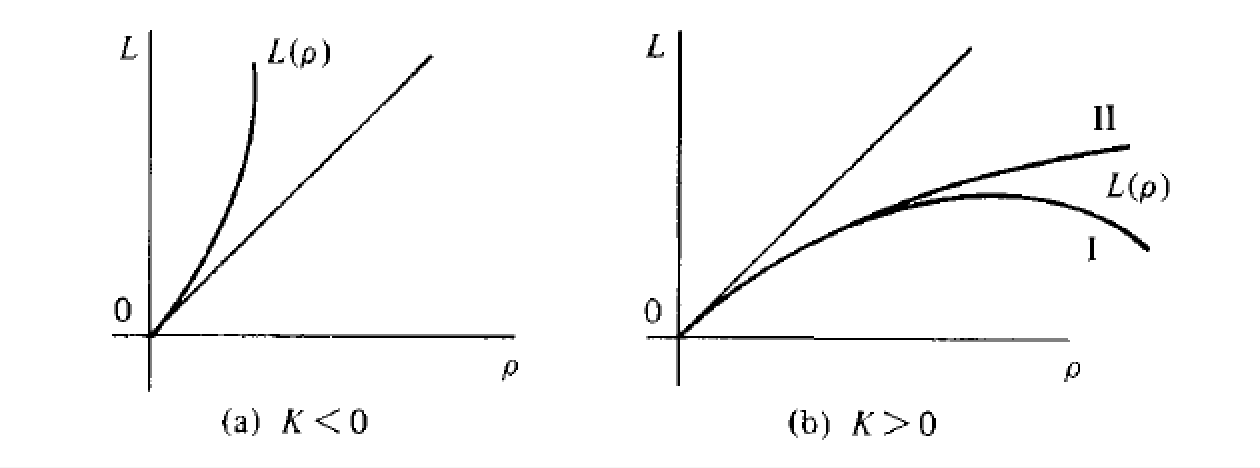
\includegraphics[scale = 0.43]{arc_length_geodesic.png}}
\end{minipage}
\end{figure}
\end{itemize}
\end{itemize}
\subsection{Geodesic and its computation via Riemannian metric and calculus of variations}
\begin{itemize}
\item  In Riemannian manifold with the metric $\mb{J} = [g_{i,j}]= \brac{\inn{\mb{x}_{\xi_{i}}}{\mb{x}_{\xi_{j}}}}$, the Lagrangian functional is defined using the \emph{Energy functional} (see exercise), $S(\xi_{1},\ldots, \xi_{n}) = \int_{a}^{b}L\paren{t, \set{\frac{d\xi^{i}}{dt}}} dt$ where
\begin{align*}
L\paren{t, \set{\frac{d\xi^{i}}{dt}}} &= \frac{1}{2}\sum_{i,j}g_{i,j}\frac{d\xi^{i}}{dt}\frac{d\xi^{j}}{dt} = \frac{1}{2}\mb{\eta}^{T}\mb{J}\,\mb{\eta}
\end{align*}  where $\mb{\eta} = [\eta_{i}] = \brac{\frac{d\xi^{i}}{dt}}.$

We solve the functional via the Euler-Lagrange equation
\begin{align*}
\partdiff{L}{\mb{\xi}} - \frac{d}{dt}\partdiff{L}{\mb{\eta}}  = \mb{0}
\end{align*}
%That is, 
%\begin{align*}
%\partdiff{L}{\mb{\xi}}&=  \frac{1}{2}\brac{\sum_{i,j}\partdiff{\mb{J}_{i,j}}{\xi_{m}} \eta_{i}\eta_{j}}_{m=1,\ldots,n}\\
%%&= \frac{1}{2}\brac{\text{tr}\paren{\partdiff{L}{\mb{J}}\partdiff{\mb{J}}{\xi_{m}}}}_{m=1,\ldots,n}\\
%%&= \frac{1}{2}\brac{\text{tr}\paren{\mb{\eta}\mb{\eta}^{T}\partdiff{\mb{J}}{\xi_{m}}}}_{m=1,\ldots,n}\\
%\partdiff{L}{\mb{\eta}}&= \mb{J}\mb{\eta}\\
%\frac{d}{dt}\partdiff{L}{\mb{\eta}} &= \paren{\frac{d}{dt}\mb{J}}\mb{\eta} + \mb{J}\dot{\mb{\eta}}\\
%&=\brac{\sum_{k=1}^{n}\partdiff{\mb{J}_{m,j}}{\xi_{k}}\eta_{k}\eta_{j}}_{m=1,\ldots,n} + \mb{J}\dot{\mb{\eta}}\\
%\dot{\mb{\eta}}%&= \mb{J}^{-1}\paren{ \frac{1}{2}\brac{\mb{\eta}^{T}\partdiff{\mb{J}}{\xi_{m}}\mb{\eta}}_{m=1,\ldots,n}- \sum_{m=1}^{n}\eta_{m}\partdiff{\mb{J}}{\xi_{m}}\mb{\eta}  }\\
%&= \mb{J}^{-1}\paren{ \frac{1}{2}\brac{\sum_{i,j}\partdiff{\mb{J}_{i,j}}{\xi_{m}}\eta_{i}\eta_{j}}_{m=1,\ldots,n}- \brac{\sum_{j,k}\partdiff{\mb{J}_{m,j}}{\xi_{k}}\eta_{k}\eta_{j}}_{m=1,\ldots,n}}\\
%&= \mb{J}^{-1}\paren{ \sum_{j=1}^{n}\eta_{j}\paren{\brac{\frac{1}{2}\sum_{i}\partdiff{\mb{J}_{i,j}}{\xi_{m}}\eta_{i}- \sum_{k}\partdiff{\mb{J}_{m,j}}{\xi_{k}}\eta_{k}}_{m=1,\ldots,n}}}    
%\end{align*}
%The system of differential equations are
%\begin{align}
%\dot{\mb{\eta}}&= \mb{J}^{-1}\mb{B}(\mb{\xi}, \mb{\eta})\mb{\eta}\nonumber\\
%\dot{\mb{\xi}} &= \mb{\eta}
%\end{align}

\item We can use metric as $\mb{J} = \brac{\inn{\mb{x}_{\xi_{i}}}{\mb{x}_{\xi_{j}}}}_{i,j}$ to derive the expression for the Christoffel symbols. Note that $\inn{\mb{N}}{\mb{x}_{\xi_{k}}} = 0,\forall k=1,\ldots, n$, so 
\begin{align}
\inn{\mb{x}_{\xi_{i}\xi_{j}}}{\mb{x}_{\xi_{m}}} &= \sum_{k}\Gamma_{i,j}^{k}\inn{\mb{x}_{\xi_{k}}}{\mb{x}_{\xi_{m}}} = \sum_{k}\Gamma_{i,j}^{k}\mb{J}_{k,m} \label{eqn: Christoffel_metric}
\end{align} 
On the other hand
\begin{align*}
\partdiff{\mb{J}_{i,m}}{\xi_{j}} &= \inn{\mb{x}_{\xi_{i}\xi_{j}}}{\mb{x}_{\xi_{m}}} + \inn{\mb{x}_{\xi_{i}}}{\mb{x}_{\xi_{m}\xi_{j}}} 
\end{align*}
Similarly
\begin{align*}
\partdiff{\mb{J}_{m,j}}{\xi_{i}} &= \inn{\mb{x}_{\xi_{i}\xi_{m}}}{\mb{x}_{\xi_{j}}} + \inn{\mb{x}_{\xi_{m}}}{\mb{x}_{\xi_{i}\xi_{j}}} \\
\partdiff{\mb{J}_{i,j}}{\xi_{m}} &= \inn{\mb{x}_{\xi_{i}\xi_{m}}}{\mb{x}_{\xi_{j}}} + \inn{\mb{x}_{\xi_{i}}}{\mb{x}_{\xi_{m}\xi_{j}}} 
\end{align*}
Thus substituting in the first equation, we have
\begin{align*}
\partdiff{\mb{J}_{i,m}}{\xi_{j}} &= \inn{\mb{x}_{\xi_{i}\xi_{j}}}{\mb{x}_{\xi_{m}}} + \inn{\mb{x}_{\xi_{i}}}{\mb{x}_{\xi_{m}\xi_{j}}} \\
&= \inn{\mb{x}_{\xi_{i}\xi_{j}}}{\mb{x}_{\xi_{m}}} +\partdiff{\mb{J}_{i,j}}{\xi_{m}}- \inn{\mb{x}_{\xi_{i}\xi_{m}}}{\mb{x}_{\xi_{j}}} \\
&=  2\inn{\mb{x}_{\xi_{i}\xi_{j}}}{\mb{x}_{\xi_{m}}} +\partdiff{\mb{J}_{i,j}}{\xi_{m}}- \partdiff{\mb{J}_{m,j}}{\xi_{i}}
\end{align*}
and 
\begin{align}
\inn{\mb{x}_{\xi_{i}\xi_{j}}}{\mb{x}_{\xi_{m}}} &= \frac{1}{2}\paren{\partdiff{\mb{J}_{j,m}}{\xi_{i}}+ \partdiff{\mb{J}_{m,i}}{\xi_{j}}  - \partdiff{\mb{J}_{i,j}}{\xi_{m}}} \label{eqn: inn_metric_diff}
\end{align}
Substituting \eqref{eqn: inn_metric_diff} into \eqref{eqn: Christoffel_metric}, we have
\begin{align}
 [ij,m]\equiv \frac{1}{2}\paren{\partdiff{\mb{J}_{j,m}}{\xi_{i}}+ \partdiff{\mb{J}_{m,i}}{\xi_{j}}  - \partdiff{\mb{J}_{i,j}}{\xi_{m}}}
 &= \sum_{k}\Gamma_{i,j}^{k}\mb{J}_{k,m};\quad  i,j,m=1,\ldots, n\label{eqn: metric_diff_eqn}
\end{align}
The above equations can be used to solve for $\Gamma_{i,j}^{k}$.

By the isometry property of Riemannian metric $\mb{J}_{i,j}$, the covariant derivative of metric tensor $\mb{x}_{\xi_{i}}^{T}\mb{J}_{i,j}\mb{x}_{\xi_{j}}$ relative to $\xi_{m}$  vanishes. That is,
\begin{align}
0=D_{\xi_{m}}\mb{J}_{i,j} &=\partdiff{\mb{J}_{i,j}}{\xi_{m}} - \sum_{s=1}^{n}\Gamma_{i,m}^{s}\mb{J}_{s,j}- \sum_{s=1}^{n}\Gamma_{m,j}^{s}\mb{J}_{i,s},\;\quad i,j,m=1,\ldots,n. \label{eqn: Christoffel_metric_eqn}
\end{align}
It can be used to solve the Christoffel symbols as 
\begin{align}
\Gamma_{i,j}^{k} &= \frac{1}{2}\sum_{m}\mb{J}^{k,m}\set{\partdiff{\mb{J}_{j,m}}{\xi_{i}}+ \partdiff{\mb{J}_{m,i}}{\xi_{j}}  - \partdiff{\mb{J}_{i,j}}{\xi_{m}}} \label{eqn: Christoffel_metric_expr}
\end{align}
where $\sum_{m}\mb{J}^{k,m}\mb{J}_{m,j}=\delta_{k}(j).$
Therefore, given the Riemannian metric in $\cS$, there exist unique covariant derivative or connection in $\cS$, which is called the \emph{Levi-Civita connection} of \emph{the Riemannian structure}.  
\end{itemize}

\newpage
\section{Homework and Examples}
\begin{itemize}
\item  \begin{example}
Define a regular surface $\cS$ as the graph of a differentiable function $h(x,y): U \subset \bR^{2} \rightarrow \bR$ for an open set $U$ of $\bR^{2}$ with $(x,y)\in U$, i.e. define the parameterization as $\mb{x}(u,v) = (u,v, h(u,v)), (u,v)\in U$. Compute the shape operator $dN_{p}$, the second fundamental form $\Pi_{p}(\mb{v})$, the Gaussian curvature $\mb{K}$ and the mean curvature $\mb{H}$.
\end{example}
\begin{figure}[thb]
\centering
\begin{minipage}{0.5\linewidth}
 \centerline{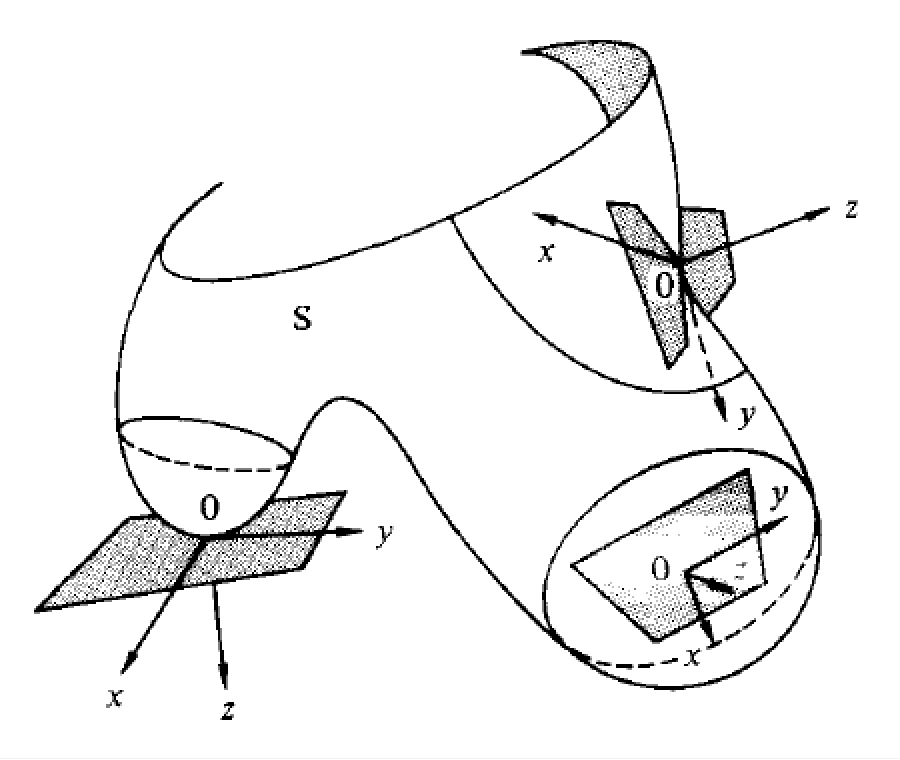
\includegraphics[scale = 0.5]{hessian_fund.png}}
\end{minipage}
\caption{\scriptsize
\textbf{Within the neighborhood of each point of the surface, we can define the function $h$ so that the surface is the graph of this function.}}
\end{figure}

For the regular surface as the graph of a function $\cS = (x,y, f(x,y)) \subset \bR^{3}$ with $h(0,0)= 0, h_{x}(0,0)=0, h_{y}(0,0) = 0$ (i.e. $xy$-plane is the tangent plane $T_{p}S$), the second fundamental form of $\cS$ at $p$ applied to the vector $(x,y)$ is 
\begin{align*}
\brac{\begin{array}{c}
x \\ 
y
\end{array} }^{T}\brac{\begin{array}{cc}
h_{xx}(0,0) & h_{xy}(0,0) \\ 
h_{yx}(0,0) & h_{yy}(0,0)
\end{array} }\brac{\begin{array}{c}
x \\ 
y
\end{array} }
\end{align*} and it is the Hessian of $h$ at $(0,0)$.\\[20pt]

\item \begin{example}
Show that if $\mb{x}$ is an orthogonal parameterization, i.e. $F=0$, then 
\begin{align*}
\mb{K} &= -\frac{1}{2\sqrt{EG}}\set{\paren{\frac{E_{v}}{\sqrt{EG}}}_{v} + \paren{\frac{G_{u}}{\sqrt{EG}}}_{u} }.\\[10pt]
\end{align*}
\end{example}

\newpage
\item \begin{example}
Let $h: \cS \rightarrow \bR$ be a differentiable function on surface $\cS$, and let $p\in \cS$ be a critical point of $h$, i.e. $dh_{p} = 0$. Let $\mb{w}\in T_{p}\cS$ and let $\alpha: (-\epsilon, \epsilon) \rightarrow \cS$ be a parameterized curve with $\alpha(0) = p$ and $\alpha'(0)= \mb{w}$. 
\begin{definition}
The quadratic form 
\begin{align*}
H_{p}h(\mb{w}) &= \rlat{\frac{d^{2} \paren{h\circ \alpha}}{dt^{2}}}{t=0}.
\end{align*}  is referred as the \emph{Hessian of $h$ at $p$}.
\end{definition} 
\begin{enumerate}
\item Let $\mb{x}: U\rightarrow \cS$ be a parameterization of $\cS$ at $p$, and show that (the fact that $p$ is a critical point here is important here)
\begin{align*}
H_{p}h(u'\mb{x}_{u}+ v'\mb{x}_{v}) &= h_{uu}(p)\paren{u'}^{2} + 2h_{uv}(p)u'v'+ h_{vv}(p)\paren{v'}^{2}.\\[5pt]
\end{align*} Conclude that $H_{p}h: T_{p}S \rightarrow \bR$ is a well-defined (i.e. it does not depend on the choice of $\alpha$) quadratic form on $T_{p}S$.

\item \begin{definition} Let $h: \cS \rightarrow \bR$ be the \emph{height} function of $\cS$ relative to $T_{p}S$; that is, $h(q)= \inn{q-p}{N(p)}, q\in 
\cS$.  \end{definition} 
Verify that $p$ is critical point of $h$ and thus that the Hessian $H_{p}h$ is well defined. Show that if $\mb{w}\in T_{p}S$, $\norm{\mb{w}}{} = 1$, then 
\begin{align*}
H_{p}h(\mb{w}) &= \text{ normal curvature at }p\text{ in the direction of }\mb{w}.
\end{align*}
Conclude that \emph{the Hessian at $p$ of the height function relative to $T_{p}S$ is the second fundamental form of $\cS$ at $p$}.\\[10pt]
\end{enumerate}
\end{example}

\item  \begin{definition}
Define \emph{the derivative $\mb{w}(f)$ of a differentiable function $f: U\subset \cS \rightarrow \bR$ relative to a vector field} $\mb{w}$ in $U$ by 
\begin{align*}
\mb{w}(f)(q) &= \rlat{\frac{d}{dt}\paren{f\circ \alpha}}{t=0},\quad q\in U
\end{align*}
where $\alpha: I\rightarrow \cS$ is the trajectory of $\mb{w}$ passing through $q$ such that $\alpha(0) = q, \alpha'(0)=\mb{w}(q)$. \end{definition}
\begin{example} Prove that 
\begin{enumerate}
\item $\mb{w}$ is differentiable in $U$ if and only if $\mb{w}(f)$ is differentiable for all differentiable function $f$ in $U$.
\item Let $\lambda, \mu\in \bR$ and $g: U\subset \cS \rightarrow \bR$ be a differentiable function on $U$ then 
\begin{align*}
\mb{w}\paren{\lambda\,f+ \mu\, g} &= \lambda\,\mb{w}(f) + \mu\,\mb{w}(g),\\
\mb{w}\paren{fg} &= \mb{w}(f)g +f\mb{w}(g).
\end{align*}
\end{enumerate}
\end{example}
Note that if $\mb{w} = \partdiff{}{u}$, then $\paren{\partdiff{}{u}}(f)(q) = \partdiff{f}{u}(q)$, which justify the notion.\\

\newpage
\item \begin{example}\citep{do1976differential} (p439.)
(The tangent bundle as a smooth manifold of dimension $2n$) \\
Consider the surface in $\mb{R}^{3}$ with parameterization $\mb{x}: U \subset \bR^{2}\rightarrow \cS$. \begin{definition}The set $T\cS \equiv \set{(p, \mb{v}): \mb{v}\in T_{p}\cS}$ where $T_{p}\cS$ is the tangent space at $p$ is called the \emph{tangent bundle}.  \end{definition}

The tangent bundle equips with a natural parameterization  $\mb{y}: U \times \bR^{2} \rightarrow T\cS$ by 
\begin{align*}
\mb{y}(u, v, w', z') &= \paren{\mb{x}(u,v),  w'\mb{x}_{u} + z'\mb{x}_{v}}  = \paren{p, \mb{v}},\quad (w',z')\in \bR^{2}
\end{align*} 
where $(u,v)$ is the coordinate of $p$ in $\cS$ and $(w',v')$ is the coordinate of $\mb{v}$ in $T_{p}\cS$.  

We can check the pair $\paren{ U \times \bR^{2},  \mb{y}}$ is a differentiable structure for $T\cS$. Note that $d\mb{x}_{q}(\bR^{2}) = T_{\mb{x}(q)}\cS, q\in U$. If $(p, \mb{v}) \in \mb{y}_{a}(U_{a}\times \bR^{2}) \cap \mb{y}_{b}(U_{b}\times \bR^{2}) $, then
\begin{align*}
\bigcup_{a}\mb{y}_{a}(U_{a}\times \bR^{2}) = T\cS
\end{align*}
since $\bigcup_{a}\mb{x}_{a}(U_{a}) = \cS$ and $(d\mb{x}_{a})_{q}(\bR^{2}) = T_{\mb{x}(q)}\cS, q\in U$.
Also, when
\begin{align*}
(p, \mb{v})  &= (\mb{x}_{a}(q_{a}),  d\mb{x}_{a}(\mb{w}_{a})) = (y_{b}(q_{b}), d\mb{x}_{b}(\mb{w}_{b}))
\end{align*}
where $q_{a}\in U_{a}$ and $q_{b}\in U_{b}$, $\mb{w}_{a}, \mb{w}_{b}\in \bR^{2}$,  
\begin{align*}
\mb{y}_{b}^{-1}\circ \mb{y}_{a}(q_{a}, \mb{w}_{a}) &= \mb{y}_{b}^{-1}\paren{\mb{x}_{a}(q_{a}),  d\mb{x}_{a}(\mb{w}_{a})}\\
&= \paren{ \mb{x}_{b}^{-1}\circ\mb{x}_{a}(q_{a}), d(\mb{x}_{b}^{-1}\circ \mb{x}_{a})(\mb{w}_{a})  }.
\end{align*}
Since $(\mb{x}_{b}^{-1}\circ\mb{x}_{a})$ is differentiable, so is $d(\mb{x}_{b}^{-1}\circ\mb{x}_{a})$. It follows that $\mb{y}_{b}^{-1}\circ \mb{y}_{a}$ is differentiable. 

The tangent bundle is a natural space to be considered by dealing with second-order ordinary differential equations (e.g. in describing the geodesic on $\cS$ ) 
\begin{align*}
\frac{d^{2}u}{dt^{2}} &= f_{1}\paren{u, v, \frac{du}{dt}, \frac{dv}{dt}}\\
\frac{d^{2}v}{dt^{2}} &= f_{2}\paren{u, v, \frac{du}{dt}, \frac{dv}{dt}}.
\end{align*}
By introducing $\frac{du}{dt} = w'$ and $\frac{dv}{dt} = z'$,  it becomes a system of first-order differential equations
\begin{align*}
\frac{du}{dt} &= w'\\
\frac{dv}{dt} &= z'\\
\frac{dw'}{dt} &= f_{1}\paren{u, v, w', z'}\\
\frac{dz'}{dt} &= f_{2}\paren{u, v, w', z'}
\end{align*}
and the solution is the trajectory of vector field $(u, v, w', v')$ given locally in the tangent bundle $T\cS$. It can be shown that such a vector field is well-defined in $T\cS$; that is, in the intersection of two coordinate neighborhoods, the vector fields in above equations agree. 

\begin{definition} This field or trajectory $(u(t), v(t), w'(t), v'(t))$ is called the \emph{geodesic flow} on $T\cS$. It is a natural object to study global properties of the geodesic on $\cS$.
\end{definition}
\end{example}


\newpage
\item  \begin{example} \citep{do1976differential} (p296. 12.)\\
A diffeomorphism $\varphi: \cS_{1} \rightarrow \cS_{2}$ is said to be a \emph{geodesic mapping} if for every geodesic $\cC\subset \cS_{1}$ of $\cS_{1}$, the regular curve $\varphi\paren{\cC} \subset \cS_{2}$ is a geodesic of $\cS_{2}$. If $U$ is a neighborhood of $p\in \cS_{1}$, then $\varphi: U \rightarrow \cS_{2}$ is said to be a \emph{local geodesic mapping} in $p$ if there exists a neighborhood $V$ of $\varphi(p)$ in $\cS_{2}$ such that $\varphi: U\rightarrow V$ is a geodesic mapping. 
\begin{enumerate}
\item Show that if $\varphi: \cS_{1} \rightarrow \cS_{2}$ is both a geodesic mapping and a conformal mapping, then $\varphi$ is a \emph{similarity};  that is,
\begin{align*}
\inn{\mb{v}}{\mb{u}} &= \lambda\inn{d\varphi_{p}(\mb{v})}{d\varphi_{p}(\mb{w})}, \quad p\in \cS_{1}, \mb{v},\mb{w} \in T_{p}\cS_{1},
\end{align*}
where $\lambda$ is constant.  

\item Let $\bS^{2} = \set{(x,y,z) \in \bR^{3}; x^{2}+ y^{2}+ z^{2} = 1}$ be the unit sphere, $\bS^{-} = \set{(x,y,z) \in \bS^{2}; z < 0}$ be the lower hemisphere, and $P$ be the plane $z=-1$. Prove that the map (central projection) $\varphi: \bS^{-} \rightarrow P$ which takes a point $p\in \bS^{-}$ to the intersection of $P$ with the line that connects $p$ to the center of $\bS^{2}$ is a geodesic mapping. 

\item Show that a surface of constant curvature admits a local geodesic mapping into the plane for every $p\in \cS$.
\end{enumerate}
\end{example}

\newpage
\item \begin{example}\citep{do1976differential} (p307. 4.)\\
The \emph{energy} $E$ of a curve $\alpha: [a,b] \rightarrow \cS$ is defined by 
\begin{align*}
E(\alpha) &= \int_{a}^{b}\abs{\dot{\alpha}(t)}^{2}dt.
\end{align*}
\begin{enumerate}
\item Show that $\paren{\ell(\alpha)}^{2} \le (b-a)E(\alpha)$ and that the equality holds if and only if $t$ is proportional to the arc length. 

\item Conclude from the above that if $\gamma: [a,b]\rightarrow \cS$ is a minimal geodesic with $\gamma(a) = p$, $\gamma(b) = q$, then for any curve $\alpha:  [a,b]\rightarrow \cS$, joining $p$ and $q$, we have $E(\gamma) \le E(\alpha) $ with the equality holds if and only if $\alpha$ is a minimal geodesic. 
\end{enumerate}
\end{example}

\newpage
\item \begin{example}\citep{do1976differential} (p306. 3.)\\
Let $\alpha: I=[0,l]\rightarrow \cS$ be a simple, parameterized, regular curve. Consider a unit vector field $\mb{v}(t)$ along $\alpha$, with $\inn{\dot{\alpha}(t)}{\mb{v}(t)}=0$ and a mapping $\mb{x}: \bR\times I \rightarrow \cS$ given by 
\begin{align*}
\mb{x}(s,t) &= \exp_{\alpha(t)}\paren{s\mb{v}(t)}, \quad s\in \bR;\; t\in I.
\end{align*}
\begin{enumerate}
\item Show that $\mb{x}$ is differentiable in the neighborhood of $I$ in $\bR\times I$ and that $d\mb{x}$ is nonsingular in $(0,t),\;t\in I$.
\item Show that there exits $\epsilon>0$ such that $\mb{x}$ is one-to-one in the rectangle $t\in I$, $\abs{s}<\epsilon$.
\item Show that in the open set $t\in (0,l), \abs{s}<\epsilon$, $\mb{x}$ is parameterization of $\cS$, the coordinate neighborhood of which contains $\alpha((0,l))$. The coordinates thus obtained are called \emph{geodesic coordinate} (or, \emph{Fermi's coordinate}) of basis $\alpha$. Show that in such a system $F=0, E=1$. Moreover, if $\alpha$ is a geodesic parameterized by the arc length,  $G(0,t) = 1$ and $G_{s}(0,t) = 0$.
\item Establish the following analogue of the Gauss lemma. Let $\alpha: I\rightarrow \cS$ be a regularized parameterized curve and let $\gamma_{t}(s),\;t\in I$ be a family of geodesics parameterized by arc length $s$ and given by $\gamma_{t}(0)=\alpha(t), \set{\dot{\gamma}_{t}(0), \dot{\alpha}_{t}}$ is a positive orthogonal basis. Then, for a fixed $\bar{s}$, sufficiently small, the curve $t\rightarrow \gamma_{t}(\bar{s}), t\in I$, intersects all $\gamma$, orthogonally (such curves are called \emph{geodesic parallels}. )
\end{enumerate}
\end{example}

\end{itemize}
\newpage
\bibliographystyle{plainnat}
\bibliography{book_reference.bib}
\end{document}